%% Beginning of file 'sample63.tex'
%%
%% Modified 2019 June
%%
%% This is a sample manuscript marked up using the
%% AASTeX v6.3 LaTeX 2e macros.
%%
%% AASTeX is now based on Alexey Vikhlinin's emulateapj.cls 
%% (Copyright 2000-2015).  See the classfile for details.

%% AASTeX requires revtex4-1.cls (http://publish.aps.org/revtex4/) and
%% other external packages (latexsym, graphicx, amssymb, longtable, and epsf).
%% All of these external packages should already be present in the modern TeX 
%% distributions.  If not they can also be obtained at www.ctan.org.

%% The first piece of markup in an AASTeX v6.x document is the \documentclass
%% command. LaTeX will ignore any data that comes before this command. The 
%% documentclass can take an optional argument to modify the output style.
%% The command below calls the preprint style which will produce a tightly 
%% typeset, one-column, single-spaced document.  It is the default and thus
%% does not need to be explicitly stated.
%%
%%
%% using aastex version 6.3
\documentclass[twocolumn]{aastex63}


%% The default is a single spaced, 10 point font, single spaced article.
%% There are 5 other style options available via an optional argument. They
%% can be invoked like this:
%%
%% \documentclass[arguments]{aastex63}
%% 
%% where the layout options are:
%%
%%  twocolumn   : two text columns, 10 point font, single spaced article.
%%                This is the most compact and represent the final published
%%                derived PDF copy of the accepted manuscript from the publisher
%%  manuscript  : one text column, 12 point font, double spaced article.
%%  preprint    : one text column, 12 point font, single spaced article.  
%%  preprint2   : two text columns, 12 point font, single spaced article.
%%  modern      : a stylish, single text column, 12 point font, article with
%% 		  wider left and right margins. This uses the Daniel
%% 		  Foreman-Mackey and David Hogg design.
%%  RNAAS       : Preferred style for Research Notes which are by design 
%%                lacking an abstract and brief. DO NOT use \begin{abstract}
%%                and \end{abstract} with this style.
%%
%% Note that you can submit to the AAS Journals in any of these 6 styles.
%%
%% There are other optional arguments one can invoke to allow other stylistic
%% actions. The available options are:
%%
%%   astrosymb    : Loads Astrosymb font and define \astrocommands. 
%%   tighten      : Makes baselineskip slightly smaller, only works with 
%%                  the twocolumn substyle.
%%   times        : uses times font instead of the default
%%   linenumbers  : turn on lineno package.
%%   trackchanges : required to see the revision mark up and print its output
%%   longauthor   : Do not use the more compressed footnote style (default) for 
%%                  the author/collaboration/affiliations. Instead print all
%%                  affiliation information after each name. Creates a much 
%%                  longer author list but may be desirable for short 
%%                  author papers.
%% twocolappendix : make 2 column appendix.
%%   anonymous    : Do not show the authors, affiliations and acknowledgments 
%%                  for dual anonymous review.
%%
%% these can be used in any combination, e.g.
%%
%% \documentclass[twocolumn,linenumbers,trackchanges]{aastex63}
%%
%% AASTeX v6.* now includes \hyperref support. While we have built in specific
%% defaults into the classfile you can manually override them with the
%% \hypersetup command. For example,
%%
%% \hypersetup{linkcolor=red,citecolor=green,filecolor=cyan,urlcolor=magenta}
%%
%% will change the color of the internal links to red, the links to the
%% bibliography to green, the file links to cyan, and the external links to
%% magenta. Additional information on \hyperref options can be found here:
%% https://www.tug.org/applications/hyperref/manual.html#x1-40003
%%
%% Note that in v6.3 "bookmarks" has been changed to "true" in hyperref
%% to improve the accessibility of the compiled pdf file.
%%

%%%%% AUTHORS - PLACE YOUR OWN PACKAGES HERE %%%%%

% Only include extra packages if you really need them. Common packages are:
\usepackage{graphicx}	% Including figure files
\usepackage{amsmath}	% Advanced maths commands
\usepackage{amssymb}	% Extra maths symbols
%\usepackage{float}
\usepackage[normalem]{ulem}
\usepackage{booktabs}	
\usepackage{mathtools}	
%

\usepackage{color}
%\usepackage[dvipsnames]{xcolor}
%\usepackage{pdflscape} %based on guideline https://mirror.hmc.edu/ctan/macros/latex/contrib/mnras/mnras_guide.pdf
%\usepackage{lscape}
%\usepackage{rotating}
\usepackage{acronym}   
\usepackage{xspace}
\usepackage{enumitem} % to make enumerate normal nrs http://ctan.org/pkg/enumitem
\usepackage{calc}% http://ctan.org/pkg/calc
\usepackage[caption=false]{subfig}
%\usepackage{subfig} % to show figures next to each other latex
%\let\captionbox\relax
%\usepackage{graphicx,caption,subcaption,showframe}
%%\captionsetup[figure]{labelsep=space,singlelinecheck=false}
%\captionsetup[subfigure]{justification=centering}


%% If you want to create your own macros, you can do so
%% using \newcommand. Your macros should appear before
%% the \begin{document} command.
%%
\newcommand{\vdag}{(v)^\dagger}
\newcommand\aastex{AAS\TeX}
\newcommand\latex{La\TeX}

%%%%%%%%%%%%%%%%%%%%%%%%


\newcommand{\floor}[1]{\textbf{\textcolor{magenta}{[Floor: #1]}}}
\newcommand{\todo}[1]{\textcolor{red}{[To do: #1]}}
\newcommand{\question}[1]{\textcolor{OliveGreen}{[Question: #1]}}
\newcommand{\edo}[1]{\textcolor{Dandelion}{[Edo: #1]}}


\definecolor{ochre}{rgb}{0.8, 0.47, 0.13}
\newcommand{\OMG}[1]{\textcolor{magenta}{#1}} %Todo/remarks by Alejandro Vigna-Gomez
\newcommand{\avg}[1]{\textcolor{ochre}{#1}} %Todo/remarks by Alejandro Vigna-Gomez
\usepackage{outlines} % for itemize in itemize
%%\newcommand{\floor}[1]{\textcolor{blue}{#1}} %Todo/remarks by Floor
%commands 
\newcommand\Fiducial{\texttt{Fiducial }}

\newcommand\rate{\mathcal{R}}
\newcommand\COMPAS{{\sc{COMPAS }}}

\newcommand{\standard}{\texttt{standard }}
\newcommand{\pluseq}{\mathrel{+}=}
%-- Constants
%\newcommand\hubbleTimeGyrs{14.6353}
\newcommand{\NEhits}{$N_{\text{T,expl}}$ }
\newcommand{\NE}{$N_{\text{expl}}$ }

\newcommand\hubbleTimeGyrs{14.03}



%BHBH mergers
\newcommand\bhns{BH--NS }
\newcommand\nsbh{NS--BH }
\newcommand\bhnsor{BH--NS or NS--BH } 
\newcommand\bhnsand{BH--NS and NS--BH }
\newcommand\bhnsSingle{BHNS\xspace}

% BNS mergers 
\newcommand\fexplOne{$  35(11) $}
\newcommand\EffExplOne{$ 35(11) $}
\newcommand\EffRefOne{$ 35(11) $}
\newcommand\NxMCOne{$  644  $}
\newcommand\NxAISOne{$ 5 (2) \%  $}
\newcommand\gainOne{$ 811 (297)  / 27688  $}
%\newcommand\UncertOne{$1.89 \, 10^{-5}$}



\newcommand\fexplTwo{$58(30)$}
\newcommand\EffExplTwo{$20(14)$}
\newcommand\EffRefTwo{$8(6)$}
\newcommand\NxMCTwo{$1000$}
\newcommand\NxAISTwo{$ 6 (3) \% $}
\newcommand\gainTwo{$1858 (902) / 39753$}

%BH-NS mergers:
\newcommand\fexplThree{$ 51(14)$}
\newcommand\EffExplThree{$7(7)$}
\newcommand\EffRefThree{$2(3)$}
\newcommand\NxMCThree{$517$}
\newcommand\NxAISThree{$10(3) \%$}
\newcommand\gainThree{$1938(383) / 21930$}

%NSNS mergers
\newcommand\fexplFour{$69(42)$}
\newcommand\EffExplFour{$40(26)$}
\newcommand\EffRefFour{$15(10)$}
\newcommand\NxMCFour{$1240$}
\newcommand\NxAISFour{$6(3) \%$}
\newcommand\gainFour{$2546 (1514) / 51442$}

% BHBH mergers with Mtot > 50Msun
\newcommand\fexplFive{$ 6 (3)$}
\newcommand\EffExplFive{$3(2)$}
\newcommand\EffRefFive{$2(1)$}
\newcommand\NxMCFive{$87$}
\newcommand\NxAISFive{$7(3) \%$}
\newcommand\gainFive{$117(67) / 1487$}

% NSNS mergers with t_coal < 50Myr
\newcommand\fexplSix{$49(32)$}
\newcommand\EffExplSix{$29(19)$}
\newcommand\EffRefSix{$14(9)$}
\newcommand\NxMCSix{$541$}
\newcommand\NxAISSix{$9(6) \%$}
\newcommand\gainSix{$1151(745) / 12653$}

% NSNS mergers with t_coal < 50Myr
\newcommand\fexplSeven{$72(32)$}
\newcommand\EffExplSeven{$35(19)$}
\newcommand\EffRefSeven{$1(1)$}
\newcommand\NxMCSeven{$1513$}
\newcommand\NxAISSeven{$5(2) \%$}
\newcommand\gainSeven{$3007 (1479)  / 80116$}

\newcommand\NtotBinaries{$29 \cdot 10^6$\xspace}
\newcommand\NtotBHNS{1076538}

\newcommand\PercentageA{$3.0\%$\xspace}
\newcommand\PercentageB{$69.4\%$\xspace}
\newcommand\PercentageBnoCE{$4.4\%$\xspace}
\newcommand\PercentageBCE{$7.2\%$\xspace}
\newcommand\PercentageC{$5.1\%$\xspace}
\newcommand\PercentageCCE{$1.0\%$\xspace}
\newcommand\PercentageDCCE{$8.7\%$\xspace}
\newcommand\PercentageOther{$1.3\%$\xspace}

\newcommand\PercentageStable{$77.5\%$\xspace}
\newcommand\PercentageImmediateCE{$8.1\%$\xspace}
\newcommand\nBPSmodels{$10$\xspace}
\newcommand\nMSSFRmodels{$28$\xspace}
%\newcommand{\kms}{\ensuremath{\,\rm{km}\,\rm{s}^{-1}}}
%\newcommand{\msun}{\,\mathrm{M}_\odot}


\newcommand\rateObsBHBH{$210$\xspace}
\newcommand\rateObsBHNS{$7$\xspace}
\newcommand\rateObsNSNS{$1$\xspace}

\newcommand\rateDetBHBH{$25$\xspace}
\newcommand\rateDetBHNS{$28$\xspace}
\newcommand\rateDetNSNS{$38$\xspace}



\newcommand{\monei}{\ensuremath{m_{1,\rm{i}}}\xspace}
\newcommand{\mtwoi}{\ensuremath{m_{2,\rm{i}}}\xspace}
\newcommand{\monef}{\ensuremath{m_{1,\rm{f}}}\xspace}
\newcommand{\mtwof}{\ensuremath{m_{2,\rm{f}}}\xspace}
\newcommand{\ai}{\ensuremath{a_{\rm{i}}}\xspace}
\newcommand{\qi}{\ensuremath{q_{\rm{i}}}\xspace}
\newcommand{\Zi}{\ensuremath{Z_{\rm{i}}}\xspace}
\newcommand{\vk}{\ensuremath{v_{\rm{k}}}\xspace}
\newcommand{\thetak}{\ensuremath{{\theta}_{\rm{k}}}\xspace}
\newcommand{\phik}{\ensuremath{{\phi}_{\rm{k}}}\xspace}
\newcommand{\ei}{\ensuremath{{e}_{\rm{i}}}\xspace}

\newcommand{\Rsun}{\ensuremath{\,\rm{R}_{\odot}}\xspace}
\newcommand{\km}{\ensuremath{\,\rm{km}}\xspace}
\newcommand{\kms}{\ensuremath{\,\rm{km}\,\rm{s}^{-1}}\xspace}
\newcommand{\Msun}{\ensuremath{\,\rm{M}_{\odot}}\xspace}
\newcommand{\Lsun}{\ensuremath{\,\rm{L}_{\odot}}\xspace}
\newcommand{\kpc}{\ensuremath{\,\rm{kpc}}\xspace}
\newcommand{\Zsun}{\ensuremath{\,\rm{Z}_{\odot}}\xspace}


%\newcommand{\fbin}{\ensuremath{f_{\rm{bin}}}}
%\newcommand{\vdag}{(v)^\dagger}
\newcommand{\AU}{\ensuremath{\,\mathrm{AU}}\xspace}
\newcommand{\Myr}{\ensuremath{\,\mathrm{Myr}}\xspace}
\newcommand{\yr}{\ensuremath{\,\mathrm{yr}}\xspace}
\newcommand{\yrs}{\ensuremath{\,\mathrm{yrs}}\xspace}
\newcommand{\Myrs}{\ensuremath{\,\mathrm{Myrs}}\xspace}
\newcommand{\Gyr}{\ensuremath{\,\mathrm{Gyr}}\xspace}
\newcommand{\Gyrs}{\ensuremath{\,\mathrm{Gyrs}}\xspace}
\newcommand{\Kelvin}{\ensuremath{\,\mathrm{K}}\xspace}
\newcommand{\yearmin}{\ensuremath{\,\rm{yr}^{-1}}\xspace}
\newcommand{\MpcminThree}{\ensuremath{\,\rm{Mpc}^{-3}}\xspace}
\newcommand{\GpcminThree}{\ensuremath{\,\rm{Gpc}^{-3}}\xspace}

\newcommand{\Hubblemin}{\ensuremath{\mathcal{H}_0^{-1}}\xspace}
\newcommand{\Hubble}{\ensuremath{\mathcal{H}_0}\xspace}

\newcommand{\MSFR}{\ensuremath{{M}_{\rm{SFR}}}\xspace}
\newcommand{\tdelay}{\ensuremath{{t}_{\rm{delay}}}\xspace}
\newcommand{\tDCO}{\ensuremath{{t}_{\rm{DCO}}}\xspace}
\newcommand{\ts}{\ensuremath{{t}_{\rm{s}}}\xspace}
\newcommand{\tevolve}{\ensuremath{{t}_{\rm{evolve}}}\xspace}
\newcommand{\tform}{\ensuremath{{t}_{\rm{form}}}\xspace}
\newcommand{\tmerger}{\ensuremath{{t}_{\rm{m}}}\xspace}
\newcommand{\tinspiral}{\ensuremath{{t}_{\rm{inspiral}}}\xspace}
\newcommand{\thubble}{\ensuremath{{t}_{\mathcal{H}}}\xspace}
\newcommand{\tdet}{\ensuremath{{t}_{\rm{det}}}\xspace}
\newcommand{\Nform}{\ensuremath{{N}_{\rm{form}}}\xspace}
\newcommand{\Ndet}{\ensuremath{{N}_{\rm{det}}}\xspace}
\newcommand{\Nmerger}{\ensuremath{{N}_{\rm{merger}}}\xspace}

\newcommand{\Pdet}{\ensuremath{{P}_{\rm{det}}}\xspace}
\newcommand{\fbin}{\ensuremath{{f}_{\rm{bin}}}\xspace}


\newcommand{\Mchirp}{\ensuremath{{\mathcal{m}}_{\rm{chirp}}}\xspace}
\newcommand{\Vc}{\ensuremath{{V}_{\rm{c}}}\xspace}
\newcommand{\DL}{\ensuremath{{D}_{\rm{L}}}\xspace}
\newcommand{\Dc}{\ensuremath{{D}_{\rm{c}}}\xspace}
%$M_{\rm{SFR}}$  $t_{\rm{delay}} = t_{\rm{form}}  + t_{\rm{merger}}$
%\ts d \Vc
\newcommand\myeq{\stackrel{\mathclap{\normalfont\mbox{def}}}{=}}
\newcommand*\diff{\mathop{}\!\mathrm{d}}

\newcommand{\CMP}{C20}


% final properties of BHNS mergers:
\newcommand{\mnsf}{\ensuremath{m_{\rm{NS}}}\xspace}
\newcommand{\mbhf}{\ensuremath{m_{\rm{BH}}}\xspace}
\newcommand{\mtotf}{\ensuremath{m_{\rm{tot}}}\xspace}
\newcommand{\mchirpf}{\ensuremath{{\mathcal{M}}_{\rm{c}}}\xspace}
\newcommand{\af}{\ensuremath{a_{\rm{f}}}\xspace}
\newcommand{\qf}{\ensuremath{q_{\rm{f}}}\xspace}
\newcommand{\ef}{\ensuremath{{e}_{\rm{f}}}\xspace}
\newcommand{\chibh}{\ensuremath{{\chi}_{\rm{BH}}}\xspace}

\newcommand{\mAzero}{\ensuremath{\rm{A}000}\xspace}
\newcommand{\mAxyz}{\ensuremath{\rm{A}xyz}\xspace}
\newcommand{\mxyz}{\ensuremath{\rm{M}xyz}\xspace}       

%-- abbreviations
%List of abbreviations
\acrodef{DNS}{double neutron star}
\acrodef{DCO}{double compact object}
\acrodef{NS}{neutron star}
\acrodef{BH}{black hole}
\acrodef{BH--NS}{black hole-neutron star}
\acrodef{GRB}{gamma--ray burst}
\acrodef{RLOF}{Roche-lobe overflow}
\acrodef{CE}{common envelope}


\acrodef{GW}{gravitational wave}
\acrodef{SN}{supernova}
\acrodefplural{SN}[SNe]{supernovae}
\acrodef{ECSN}{electron-capture SN}
\acrodef{PISN}{pair-instability SN}
\acrodefplural{ECSN}[ECSNe]{electron-capture SN}
\acrodef{USSN}{ultra-stripped SN}
\acrodefplural{USSN}[USSNe]{ultra-stripped SN}
\acrodef{CCSN}{core-collapse SN}
\acrodefplural{CCSN}[CCSNe]{core-collapse SN}
\acrodef{COMPAS}{
Compact Object Mergers: Population Astrophysics and Statistics}
\acrodef{MSSFR}{metallicity-specific star formation rate}


%%%%%%%%%%%%%%%%%%%%%%%%


%% Reintroduced the \received and \accepted commands from AASTeX v5.2
\received{XX}
\revised{XX}
\accepted{XX}
%% Command to document which AAS Journal the manuscript was submitted to.
%% Adds "Submitted to " the argument.
\submitjournal{AJ}

%% For manuscript that include authors in collaborations, AASTeX v6.3
%% builds on the \collaboration command to allow greater freedom to 
%% keep the traditional author+affiliation information but only show
%% subsets. The \collaboration command now must appear AFTER the group
%% of authors in the collaboration and it takes TWO arguments. The last
%% is still the collaboration identifier. The text given in this
%% argument is what will be shown in the manuscript. The first argument
%% is the number of author above the \collaboration command to show with
%% the collaboration text. If there are authors that are not part of any
%% collaboration the \nocollaboration command is used. This command takes
%% one argument which is also the number of authors above to show. A
%% dashed line is shown to indicate no collaboration. This example manuscript
%% shows how these commands work to display specific set of authors 
%% on the front page.
%%
%% For manuscript without any need to use \collaboration the 
%% \AuthorCollaborationLimit command from v6.2 can still be used to 
%% show a subset of authors.
%
%\AuthorCollaborationLimit=2
%
%% will only show Schwarz & Muench on the front page of the manuscript
%% (assuming the \collaboration and \nocollaboration commands are
%% commented out).
%%
%% Note that all of the author will be shown in the published article.
%% This feature is meant to be used prior to acceptance to make the
%% front end of a long author article more manageable. Please do not use
%% this functionality for manuscripts with less than 20 authors. Conversely,
%% please do use this when the number of authors exceeds 40.
%%
%% Use \allauthors at the manuscript end to show the full author list.
%% This command should only be used with \AuthorCollaborationLimit is used.

%% The following command can be used to set the latex table counters.  It
%% is needed in this document because it uses a mix of latex tabular and
%% AASTeX deluxetables.  In general it should not be needed.
%\setcounter{table}{1}

%%%%%%%%%%%%%%%%%%%%%%%%%%%%%%%%%%%%%%%%%%%%%%%%%%%%%%%%%%%%%%%%%%%%%%%%%%%%%%%%
%%
%% The following section outlines numerous optional output that
%% can be displayed in the front matter or as running meta-data.
%%
%% If you wish, you may supply running head information, although
%% this information may be modified by the editorial offices.
\shorttitle{Characteristics of BHNS mergers}
\shortauthors{Broekgaarden et al.}
%%
%% You can add a light gray and diagonal water-mark to the first page 
%% with this command:
%% \watermark{text}
%% where "text", e.g. DRAFT, is the text to appear.  If the text is 
%% long you can control the water-mark size with:
%% \setwatermarkfontsize{dimension}
%% where dimension is any recognized LaTeX dimension, e.g. pt, in, etc.
%%
%%%%%%%%%%%%%%%%%%%%%%%%%%%%%%%%%%%%%%%%%%%%%%%%%%%%%%%%%%%%%%%%%%%%%%%%%%%%%%%%

%% This is the end of the preamble.  Indicate the beginning of the
%% manuscript itself with \begin{document}.

\begin{document}

\title{Breath and depth: Predictions for  gravitational-wave observations exploring both  massive star and cosmic history uncertainties. }

%% LaTeX will automatically break titles if they run longer than
%% one line. However, you may use \\ to force a line break if
%% you desire. In v6.3 you can include a footnote in the title.

%% A significant change from earlier AASTEX versions is in the structure for 
%% calling author and affiliations. The change was necessary to implement 
%% auto-indexing of affiliations which prior was a manual process that could 
%% easily be tedious in large author manuscripts.
%%
%% The \author command is the same as before except it now takes an optional
%% argument which is the 16 digit ORCID. The syntax is:
%% \author[xxxx-xxxx-xxxx-xxxx]{Author Name}
%%
%% This will hyperlink the author name to the author's ORCID page. Note that
%% during compilation, LaTeX will do some limited checking of the format of
%% the ID to make sure it is valid. If the "orcid-ID.png" image file is 
%% present or in the LaTeX pathway, the OrcID icon will appear next to
%% the authors name.
%%
%% Use \affiliation for affiliation information. The old \affil is now aliased
%% to \affiliation. AASTeX v6.3 will automatically index these in the header.
%% When a duplicate is found its index will be the same as its previous entry.
%%
%% Note that \altaffilmark and \altaffiltext have been removed and thus 
%% can not be used to document secondary affiliations. If they are used latex
%% will issue a specific error message and quit. Please use multiple 
%% \affiliation calls for to document more than one affiliation.
%%
%% The new \altaffiliation can be used to indicate some secondary information
%% such as fellowships. This command produces a non-numeric footnote that is
%% set away from the numeric \affiliation footnotes.  NOTE that if an
%% \altaffiliation command is used it must come BEFORE the \affiliation call,
%% right after the \author command, in order to place the footnotes in
%% the proper location.
%%
%% Use \email to set provide email addresses. Each \email will appear on its
%% own line so you can put multiple email address in one \email call. A new
%% \correspondingauthor command is available in V6.3 to identify the
%% corresponding author of the manuscript. It is the author's responsibility
%% to make sure this name is also in the author list.
%%
%% While authors can be grouped inside the same \author and \affiliation
%% commands it is better to have a single author for each. This allows for
%% one to exploit all the new benefits and should make book-keeping easier.
%%
%% If done correctly the peer review system will be able to
%% automatically put the author and affiliation information from the manuscript
%% and save the corresponding author the trouble of entering it by hand.

\correspondingauthor{Floor Broekgaarden}
\email{floor.broekgaarden@cfa.harvard.edu}

\author[0000-0002-4421-4962]{Floor S. Broekgaarden}
\affiliation{Harvard-Smithsonian Center for Astrophysics,
60 Garden St., Cambridge, MA 02138, USA}


\author[0000-0002-9392-9681]{Edo Berger}
\affiliation{Harvard-Smithsonian Center for Astrophysics,
60 Garden St., Cambridge, MA 02138, USA}


%\author{Coenraad J. Neijssel}
%\affiliation{Monash Centre for Astrophysics, School of Physics and Astronomy, Monash University, Clayton, Victoria 3800, Australia}
%\affiliation{The ARC Center of Excellence for \ac{GW} Discovery -- OzGrav, Hawthorn VIC 3122, Australia}
%\affiliation{Birmingham Institute for \ac{GW} Astronomy and School of Physics and Astronomy, University of Birmingham}
%
%\author{Stephen Justham}
%\affiliation{School of Astronomy $\&$ Space Science, University of the Chinese Academy of Sciences, Beijing 100012, China}
%\affiliation{National Astronomical Observatories, Chinese Academy of Sciences, Beijing 100012, China}
%\affiliation{Anton Pannekoek Institute for Astronomy, University of Amsterdam, Postbus 94249, 1090 GE Amsterdam, The Netherlands }
%\affiliation{GRAPPA, University of Amsterdam, Science Park 904, 1098 XH Amsterdam, The
%Netherlands}
%
%\author{Alejandro Vigna-G\'{o}mez}
%\affiliation{Dark Cosmology Centre, Niels Bohr Institute, University of
%Copenhagen, Juliane Maries Vej 30, DK-2100, K\o benhaven \o, Denmark}
%
%\author{Ilya Mandel}
%\affiliation{Monash Centre for Astrophysics, School of Physics and Astronomy, Monash University, Clayton, Victoria 3800, Australia}
%\affiliation{The ARC Center of Excellence for \ac{GW} Discovery -- OzGrav, Hawthorn VIC 3122, Australia}
%

%$^{2}$Monash Centre for Astrophysics, School of Physics and Astronomy, Monash University, Clayton, Victoria 3800, Australia\\
%$^{3}$The ARC Center of Excellence for \ac{GW} Discovery -- OzGrav, Hawthorn VIC 3122, Australia\\
%$^{4}$Birmingham Institute for Gravitational Wave Astronomy and School of Physics and Astronomy, University of Birmingham \\ 
%$^{}$ Birmingham, B15 2TT, United Kingdom\\
%$^{5}$School of Astronomy $\&$ Space Science, University of the Chinese Academy of Sciences, Beijing 100012, China\\
%$^{6}$National Astronomical Observatories, Chinese Academy of Sciences, Beijing 100012, China\\
%$^{7}$Anton Pannekoek Institute for Astronomy, University of Amsterdam, Postbus 94249, 1090 GE Amsterdam, The Netherlands \\
%$^{8}$GRAPPA, University of Amsterdam, Science Park 904, 1098 XH Amsterdam, The
%Netherlands \\
%$^{9}$Dark Cosmology Centre, Niels Bohr Institute, University of
%Copenhagen, Juliane Maries Vej 30, DK-2100, K\o benhaven \o, Denmark % \\
%%$^{10}$Center for Astrophysics and Supercomputing, Swinburne University of Technology, Hawthorn VIC 3122, Australia\\
%}

%\author{Simon Stevenson}
%\affiliation{Center for Astrophysics and Supercomputing, Swinburne University of Technology, Hawthorn VIC 3122, Australia}
%\affiliation{The ARC Center of Excellence for Gravitational Wave Discovery -- OzGrav, Hawthorn VIC 3122, Australia}
%
%\author{Selma E. de Mink}
%\affiliation{Harvard-Smithsonian Center for Astrophysics,
%60 Garden St., Cambridge, MA 02138, USA}

\author{TBD}
\affiliation{Harvard-Smithsonian Center for Astrophysics,
60 Garden St., Cambridge, MA 02138, USA}


%\author[F.S. Broekgaarden et al.]
%{Floor S. Broekgaarden,$^{1}$\thanks{E-mail: floor.broekgaarden@cfa.harvard.edu}
%TBD, 
%%Edo Berger,$^{1}$
%%Coenraad J. Neijssel$^{2,3,4}$
%%Stephen Justham,$^{5,6,7,8}$
%%\newauthor
%%Alejandro Vigna-G\'{o}mez,$^{9}$
%%Ilya Mandel,$^{2,3}$
%%%Simon Stevenson,$^{3,10}$
%%%\newauthor
%% Serena Vinciguerra
%%Selma E. de Mink,$^{1,7,8}$
%\\

%\collaboration{1}{(AAS Journals Data Scientists collaboration)}
%
%\author{Butler Burton}
%\affiliation{Leiden University}
%\affiliation{AAS Journals Associate Editor-in-Chief}
%\nocollaboration{1}
%
%\author{Amy Hendrickson}
%\altaffiliation{AASTeX v6+ programmer}
%\affiliation{TeXnology Inc.}
%
%\collaboration{1}{(LaTeX collaboration)}
%
%\author{Julie Steffen}
%\affiliation{AAS Director of Publishing}
%\affiliation{American Astronomical Society \\
%1667 K Street NW, Suite 800 \\
%Washington, DC 20006, USA}
%
%\author{Scott Chernoff}
%\affiliation{IOP Publishing, Washington, DC 20005}
%
%\nocollaboration{2}

%% Note that the \and command from previous versions of AASTeX is now
%% depreciated in this version as it is no longer necessary. AASTeX 
%% automatically takes care of all commas and "and"s between authors names.

%% AASTeX 6.3 has the new \collaboration and \nocollaboration commands to
%% provide the collaboration status of a group of authors. These commands 
%% can be used either before or after the list of corresponding authors. The
%% argument for \collaboration is the collaboration identifier. Authors are
%% encouraged to surround collaboration identifiers with ()s. The 
%% \nocollaboration command takes no argument and exists to indicate that
%% the nearby authors are not part of surrounding collaborations.

%% Mark off the abstract in the ``abstract'' environment. 
\begin{abstract}


\end{abstract}

%% Keywords should appear after the \end{abstract} command. 
%% See the online documentation for the full list of available subject
%% keywords and the rules for their use.
\keywords{binaries --- gravitational waves --- 
evolution--- stars --- cosmology}

%% From the front matter, we move on to the body of the paper.
%% Sections are demarcated by \section and \subsection, respectively.
%% Observe the use of the LaTeX \label
%% command after the \subsection to give a symbolic KEY to the
%% subsection for cross-referencing in a \ref command.
%% You can use LaTeX's \ref and \label commands to keep track of
%% cross-references to sections, equations, tables, and figures.
%% That way, if you change the order of any elements, LaTeX will
%% automatically renumber them.
%%
%% We recommend that authors also use the natbib \citep
%% and \citet commands to identify citations.  The citations are
%% tied to the reference list via symbolic KEYs. The KEY corresponds
%% to the KEY in the \bibitem in the reference list below. 



%%%%%%%%%%%%%%%%%%%%%%%%%%%%%%%%%%%%%%%%%%%%%
%%%%%%%%%%%%%%%%%%%%%%%%%%%%%%%%%%%%%%%%%%%%%
%%%%%%%%%%%%%%%%%%%%%%%%%%%%%%%%%%%%%%%%%%%%%
%%%%%%%%%%%%%%%%%%%%%%%%%%%%%%%%%%%%%%%%%%%%%
%%%%%%%%%%%%               INTRODUCTION            %%%%%%%%%%%%%%%
%%%%%%%%%%%%%%%%%%%%%%%%%%%%%%%%%%%%%%%%%%%%%
%%%%%%%%%%%%%%%%%%%%%%%%%%%%%%%%%%%%%%%%%%%%%
%%%%%%%%%%%%%%%%%%%%%%%%%%%%%%%%%%%%%%%%%%%%%
%%%%%%%%%%%%%%%%%%%%%%%%%%%%%%%%%%%%%%%%%%%%%
%%%%%%%%%%%%%%%%%%%%%%%%%%%%%%%%%%%%%%%%%%%%%



\section{Introduction}
\label{sec:introduction}
%


\section{Method}
\label{sec:method}

\subsection{Predicted GW observable \bhnsSingle distributions }
\label{subsec:distributions-FIducial-GW-observable}

%
%\begin{itemize}
%	\item Chirp mass distribution
%	\item Atotal mass distribution
%	\item individual masses distribution 
%	\item  mass ratios
%	\item BH--NS mergers in aLIGO with ejecta?
%	\item 
%\end{itemize}
%
%\section{OLD}
%\label{sec:results}
%
%

%
\begin{figure}
    \centering
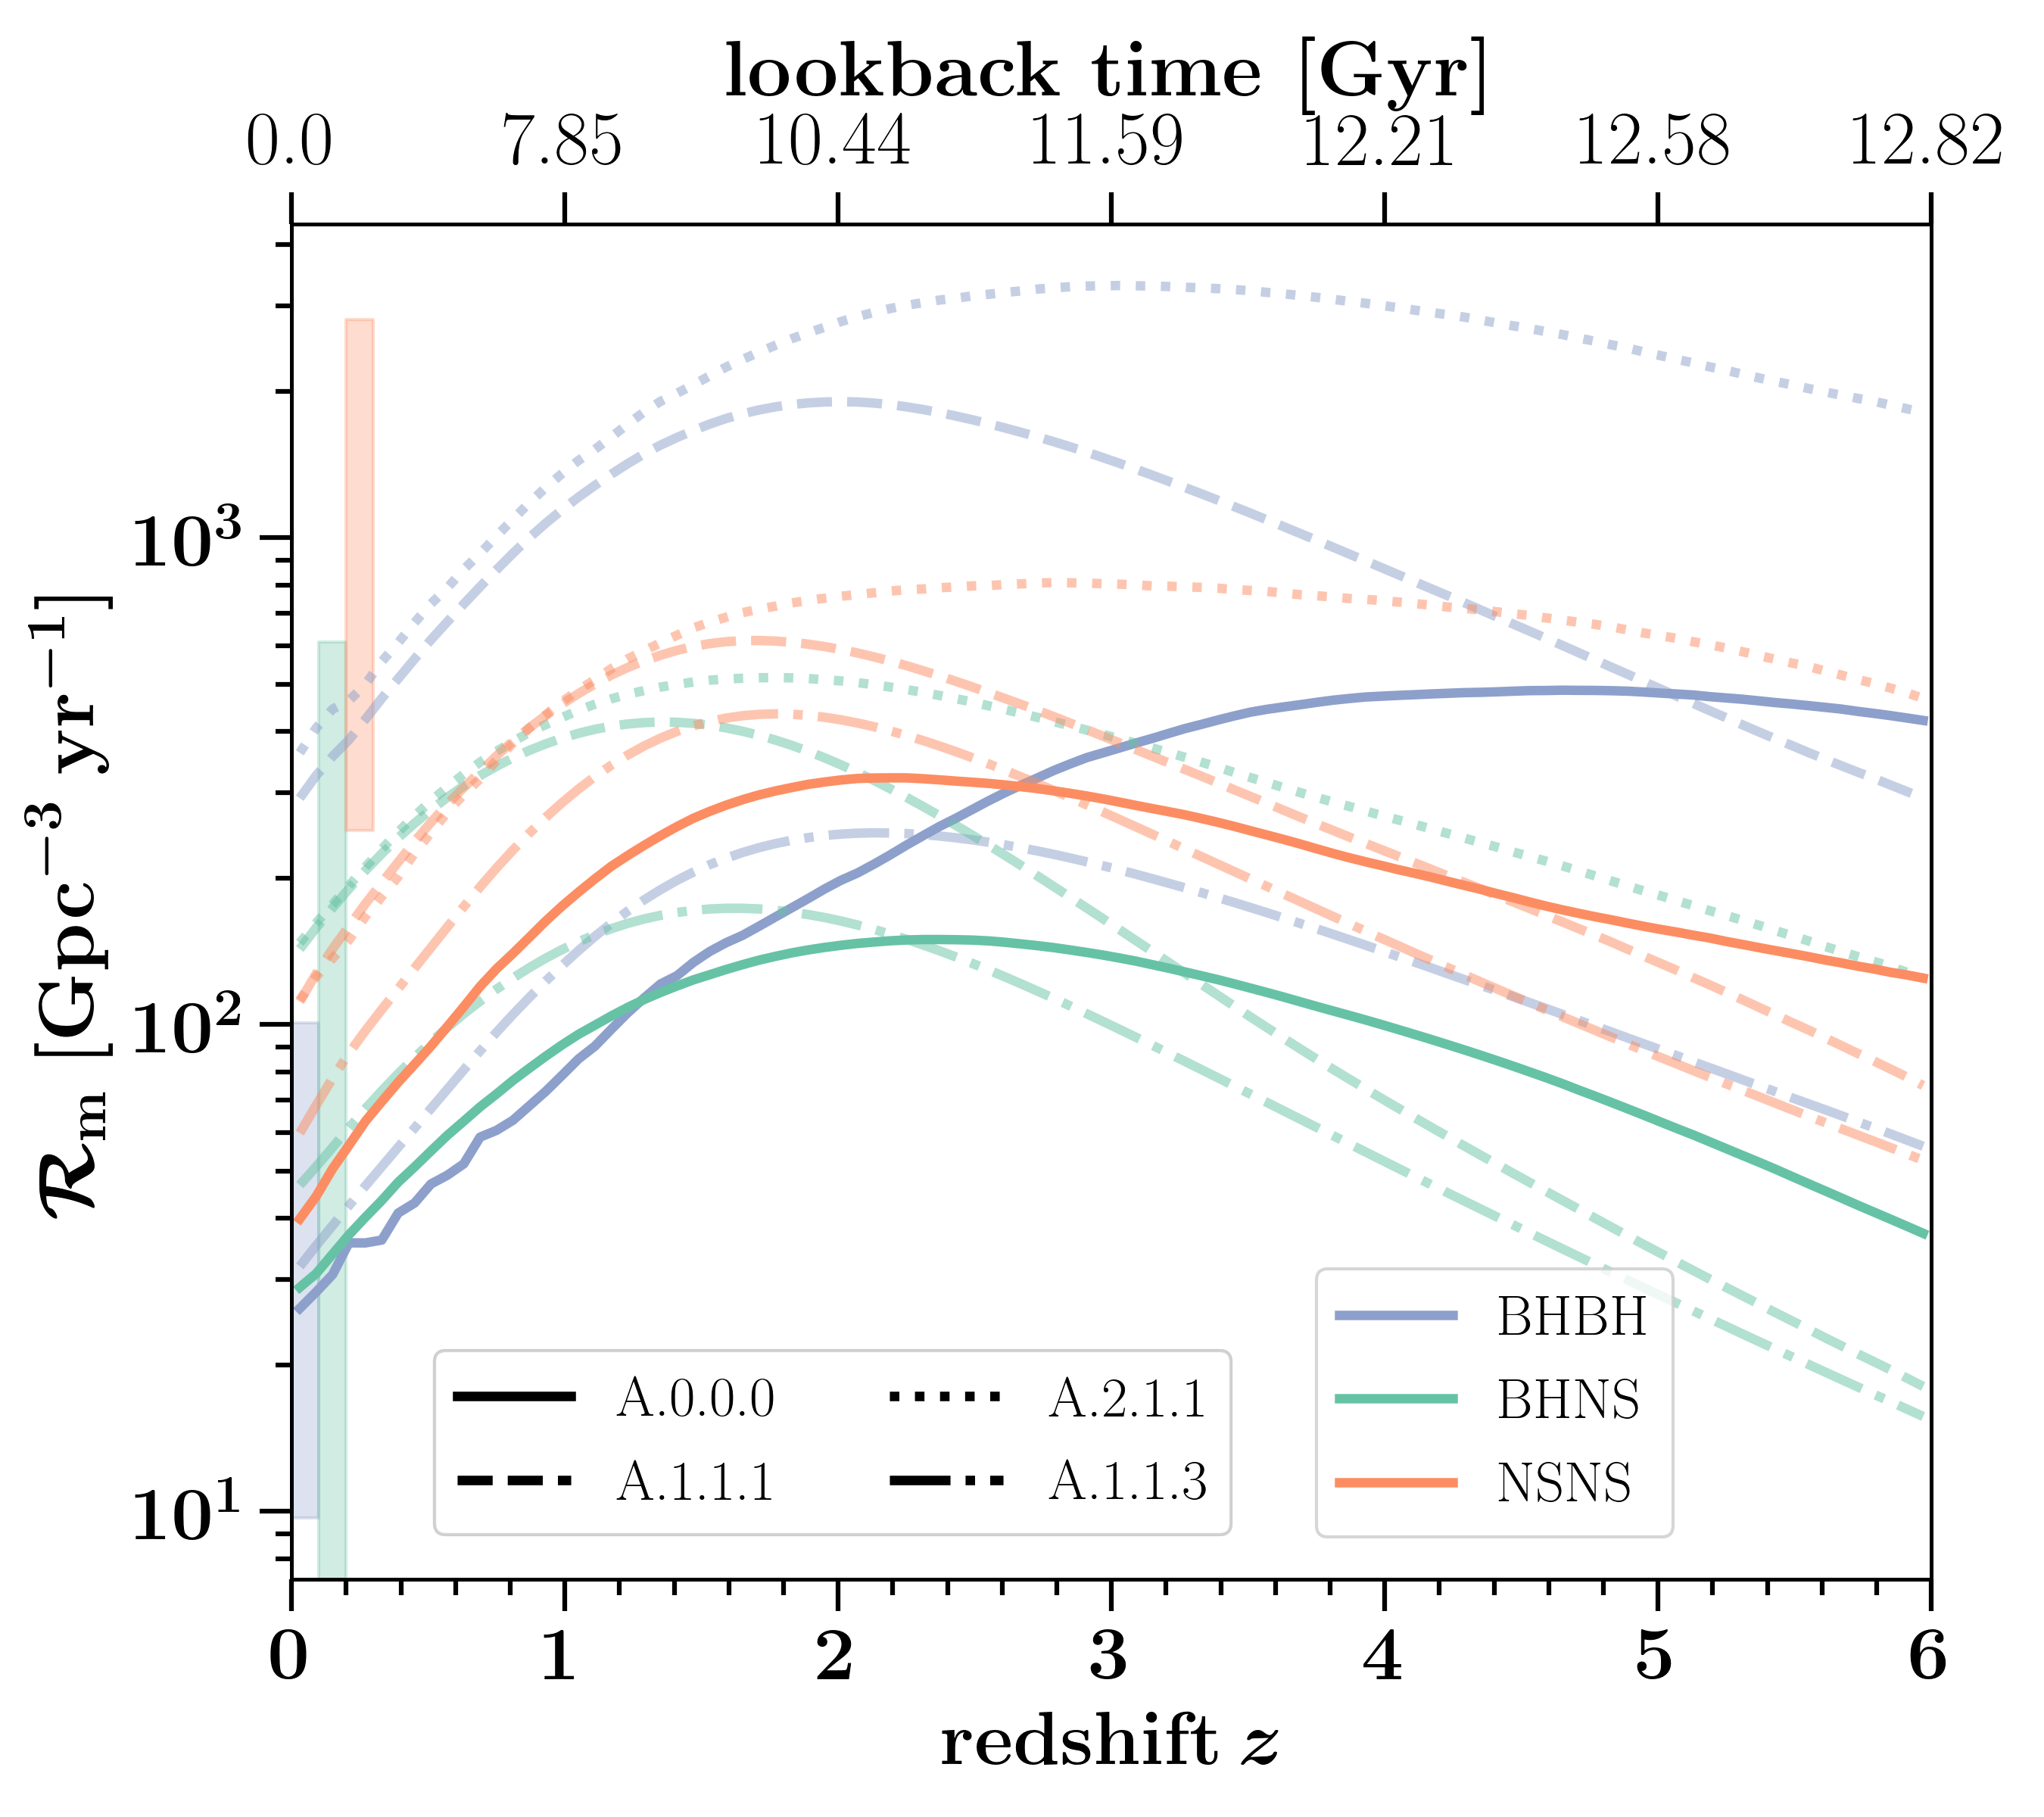
\includegraphics[width=1.0\columnwidth]{../PlottingScripts/5_DCOPerRedshift/TotalMergerRateRedshift_4_MSSFRs_ALPHA.png} %
\end{figure}
%




%%
%%
\floor{
\begin{align*}
	\text{to   Edo: I GOT UNTIL HERE \hspace{4cm}}\\
  \hline \hline 
  \end{align*}}
%%
%%






\section{Varying model assumptions}
\label{sec:results-variations}
%
The \bhnsSingle \ac{GW} predictions for the fiducial model \mAzero (Section~\ref{sec:results-fiducial}) can be sensitive to uncertainties in \ac{MSSFR} and massive star evolution which are  presented in this section. We present \nBPSmodels different population synthesis models and vary for each between \nMSSFRmodels \ac{MSSFR} prescriptions. These model variations are summarized in Table~\ref{tab:variations-BPS} and~\ref{tab-MSSFR-variations-labels}.  





\subsection{Intrinsic merger rates}
\label{subsec:results-variations-rates}
%


%%
\begin{figure*}
    \centering
\includegraphics[width=1.0\textwidth]{../PlottingScripts/8_PredictedRates_BPS_and_MSSFR_variations/Rates_intrinsic_analysisFiducialMSSFR_linestyleColouring.png} %
    \caption{Predicted intrinsic rates of BHBH, BHNS and NSNS mergers as a function of different population synthesis models (summarized in Table~\ref{tab:variations-BPS}).  
    The rates are for mergers at redshift $z=0$ without applying \ac{GW} selection effects. 
    For each binary population synthesis model the figure shows rates for the 28 variations in \ac{MSSFR} (Table~\ref{tab-MSSFR-variations-labels}). Four \ac{MSSFR} variations are highlighted.  In the background of each panel the  $90\%$ confidence interval for the observed rate by \citep{2019PhRvX...9c1040A,2020arXiv200101761T} are shown, where the \bhnsSingle is an upper limit. Our fiducial model  (\mAzero) estimates are shown with star symbols. On the right of each panel  $<\sigma_{\mu}>$ and $<\sigma_{\rm{.x.y.z}}>$ represent the mean scatter  in  rates caused over binary population synthesis and \ac{MSSFR} variations respectively. The minimum and maximum rates as well as the ratio between those are quoted for each merger type. We use the short-hand notation $\rate_{\rm{m}}^0 \equiv (\diff \Ndet^2 / \diff \ts \diff \Vc)(\tmerger(z=0))$. }%
    \label{fig:IntrinsicRates}
\end{figure*}
%



%
\begin{table}
\caption{All binary population synthesis models simulated in this study. \\
 $^{*}$total number of \bhnsSingle  mergers found in combined simulation over 30 metallicity bins }
\label{tab:variations-BPS}
\resizebox{\columnwidth}{!}{%
\centering
\begin{tabular}{lllr}
\hline
$m$ 	& Physics that is changed & Variation  			& nr$^{*}$    		\\ \hline
A      		& fiducial model        		& -     					& $1\,366\,530$    	\\
B      		&  \ac{CE}       		& optimistic     					& $1\,407\,608 $ 	\\
C       		& \ac{CE}                    				& $\alpha = 0.1$ 	& $275\,375$ 		\\
D       		& \ac{CE}                    				& $\alpha = 10$  	& $50\,208$ 		\\
E       		& case BB mass transfer 	& Unstable 			&      \\
F       		& SNe                   				& Fryer rapid   		& \\
G       		& SNe                   				& no \ac{BH} kick   		& \\
H       		& mass transfer                  				& $\beta=0.25$  		& \\ 
I       		& mass transfer                  				& $\beta=0.5$  		& \\ 
J       		& mass transfer                  				& $\beta=0.75$  		& \\ 
\hline
\end{tabular}%
}
\end{table}


The predicted intrinsic rates for BHBH, \bhnsSingle and NSNS mergers are shown for different combinations of binary population synthesis and \ac{MSSFR} models in Figure~\ref{fig:IntrinsicRates}. 
These rates are calculated using Equation~\ref{eq:MSSFR-merger-rate}  at redshift zero and do not yet take into account the \ac{GW} selection effects.  
 The intrinsic merger rates are in the ranges $\rate_{\rm{m}}^0 \sim$ [15, 694], [3, 284] and [0.6,  172] \GpcminThree \yearmin for BHBH, \bhnsSingle and NSNS mergers respectively. 
 
Most of the predicted rates in Figure~\ref{fig:IntrinsicRates} are consistent with the observed $90\%$ confidence interval of the rates from \citep{2019PhRvX...9c1040A,2020arXiv200101761T} with two exceptions.
First, a subset of the \ac{MSSFR} variations overpredicts the  BHBH merger rate for all binary population synthesis model variations. These are the \ac{MSSFR} models that have the  \citet{2006ApJ...638L..63L}   MZR ($\rm{xyz}=\rm{xy}1$). For a fixed galaxy mass, this   MZR relation results in lower metallicities compared to our other MZR options (see Appendix A of  \citealt{2019MNRAS.490.3740N} for more details) which increases the formation of \acp{BH} and thereby  BHBH mergers. 
Secondly,   almost all  predicted NSNS merger rates  are below the observed 90$\%$ confidence interval.  
 This finding is similar to other work on the isolated binary evolution channel  \citep[e.g.][]{2018MNRAS.474.2937C}. This could indicate  that the observed estimate from \ac{GW} observations might be an over-prediction caused by the small number of observations. Alternatively,   our binary population synthesis models might underestimate the efficiency of NSNS merger formation. Examples could be that  binary population synthesis underestimates the expansion of low mass stars that lead to NSs. Or because CE is more efficient .  \floor{add sGRB lines}

We note that the \ac{GW} observed rates for  NSNS mergers are larger compared to estimates from pulsars, see \citep{2018MNRAS.474.2937C} for a further discussion. 
 


To quantify the scatter in the predicted rates as a result from model variation we calculate for  the binary population synthesis models the mean of the ratios between the maximum and minimum predicted rates given by
%
\begin{equation}
<\sigma_{\rm{\mu}}> = \frac{1}{10} \sum_{\mu=A}^{\mu=J}
 \frac{\rm{max}(\rate_{\rm{m, \mu000}}^0,... ,\rate_{\rm{m, \mu333}}^0 )}{\rm{min}(\rate_{\rm{m, \mu000}}^0,... ,\rate_{\rm{m, \mu333}}^0 ) }.
\end{equation} 
%
The same is done to quantify the scatter by varying \ac{MSSFR} models
%
\begin{equation}
<\sigma_{\rm{xyz}}> = \frac{1}{28} \sum_{\rm{xyz}=000}^{\rm{xyz}=333}
 \frac{\rm{max}(\rate_{\rm{m, Axyz}}^0,... ,\rate_{\rm{m, Jxyz}}^0 )}{\rm{min}(\rate_{\rm{m, Axyz}}^0,... ,\rate_{\rm{m, Jxyz}}^0)}.
\end{equation} 
%
In addition we also quote the overall maximum and minimum rates found in our simulations in Figure~\ref{fig:IntrinsicRates}. 

The intrinsic BHBH rates only vary a factor $\sim 5$ between our model variations whereas the scatter caused by \ac{MSSFR} uncertainty is a factor $\sim 17$ as can be seen in Figure~\ref{fig:IntrinsicRates}. The optimistic \ac{CE} model (B) is an outlier and overpredicts  the observed BHBH merger rate for all \ac{MSSFR} models. 
This is different for the \bhnsSingle and NSNS rates where the scatter in predicted rates in our model variations is largest by the binary population synthesis assumptions. Especially for NSNS mergers the model variations dominate. The \ac{MSSFR}  only makes the predicted NSNS rates vary by a factor $\sim 5\times$ which is mostly because the formation yield of NSNS is not as sensitive to metallicity compared with BHBH (see Figure~\ref{fig:BHNS_rate_per_metallicity}). 

For \bhnsSingle mergers, especially models C, D, E and J lead to low merger rates. For NSNS mergers this is model E. \floor{interpertate this}

We find that the predicted rates can vary factors of $\sim 48\times $, $109\times $ and $292\times $ for BHBH \bhnsSingle and NSNS respectively. 
Future constrains from \ac{GW} observations on the predicted rates will help constrain between binary population synthesis and \ac{MSSFR} variations. Where BHBH will especially be good probes to study \ac{MSSFR} and \bhnsSingle and NSNS are probes for model variations. 


\subsection{GW detected merger rates}
\label{subsec:results-variations-rates-observed}

The predicted detected merger rate for BHBH, \bhnsSingle and NSNS mergers  are shown in Figure~\ref{fig:ObservedRates}. 
These rates are calculated using Equation~\ref{eq:rate_detector} for a ground-based \ac{GW} detector network at design sensitivity. 
Our fiducial model predicts observed rates of \rateObsBHBH, \rateObsBHNS and  \rateObsNSNS  \GpcminThree \yearmin for BHBH, \bhnsSingle and NSNS mergers respectively.

Compared to the intrinsic rates, the predicted detected rates are more sensitive to the \ac{MSSFR} prescriptions for BHBH mergers which now has an average scatter in rates of $\sigma_{\rm{.x.y.z}} \approx 44\times$. This  is because \ac{GW} detectors are more sensitive to more massive BHBH mergers that typically form only at low metallicities. The yield of those BHBH mergers, that are detectable out to larger distances, depends strongly on the \ac{MSSFR} prescription. In total we see variations in the predicted detectable merger rates of factors $\sim 93\times, 123\times, 212\times$ for BHBH, \bhnsSingle and NSNS mergers respectively. 







%
\begin{figure*}
    \centering
\includegraphics[width=1.0\textwidth]{../PlottingScripts/8_PredictedRates_BPS_and_MSSFR_variations/Rates_observed_analysisFiducialMSSFR_linestyleColouring.png} %
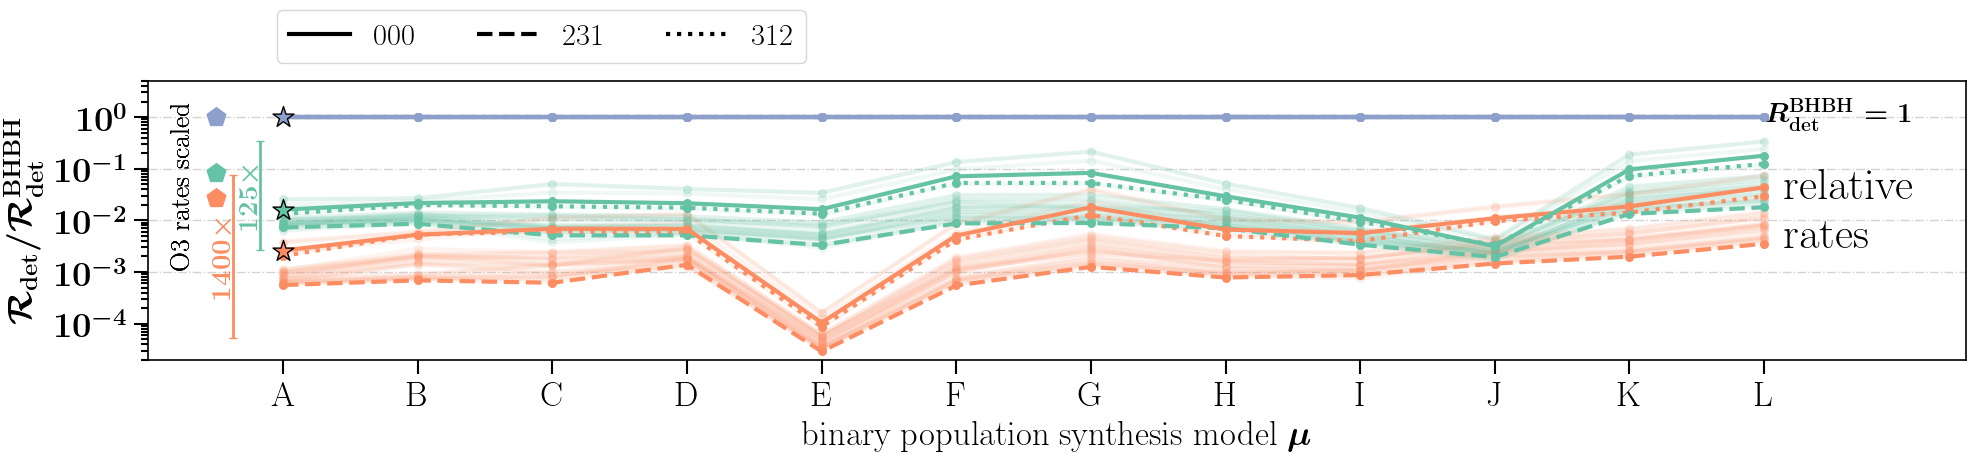
\includegraphics[width=1.0\textwidth]{../PlottingScripts/8_PredictedRates_BPS_and_MSSFR_variations/RatesRatios_observed.png} 
    \caption{Same as Figure~\ref{fig:IntrinsicRates} but now the observed rates that are obtained by taking into account the \ac{GW} selection effects (Section~\ref{subsec:detection-probability}). We use the short-hand notation $\rate_{\rm{det}} \equiv \diff \Ndet / \diff \tdet$}%
    \label{fig:ObservedRates}
\end{figure*}
%
Section \ref{subsec:results-variations-rates-observed} showed that the predicted rate of \bhnsSingle mergers can change more than three orders or magnitude by varying the \ac{MSSFR} and binary population synthesis prescriptions. In this  


\subsection{Predicted distribution functions}
%

In addition to the rate, the shape of the predicted \bhnsSingle distributions is sensitive to the \ac{MSSFR} and binary population synthesis assumptions. 
This can be seen in Figure~\ref{fig:CDFs_BHNS_observed} that shows the predicted \bhnsSingle  cumulative distribution functions for our binary population synthesis and \ac{MSSFR} variations. 

To summarize the shape of each distribution we show in Figure~\ref{fig:ConfidenceINtervals_BHNS}   the median, $50\%$, $90\%$ and $99\%$ confidence intervals for the mass distributions of \bhnsSingle mergers.  Instead of the inspiral time we show  in the last panel  the birth metallicity of the detected mergers to indicate the typical metallicities that the mergers origin from.  The inspiral time and metallicity are typically highly correlated as mergers with longer inspiral times typically are formed with lower birth  metallicities. The same distributions for  BHBH ans NSNS mergers are given in Appendix~\ref{sec:app-BHBHandNSNS_CDF}).


Overall we find that the variation in the predicted \bhnsSingle distribution functions is dominated by the binary population synthesis model. This can  be seen from the scatter in the median and  $50\%$ confidence intervals in Figure~\ref{fig:ConfidenceINtervals_BHNS} that are typically larger between models compared to between \ac{MSSFR} variations. This is different from BHBH mergers where the dominant factor is the \ac{MSSFR} assumption. 
We highlight a few results below. 




\subsubsection{MSSFR variations}
We find that the 



\subsubsection{BH mass}
 Figure~\ref{fig:ConfidenceINtervals_BHNS} shows that in all our model variations  $90\%$ of the \bhnsSingle mergers have \ac{BH} masses within the range $[2.5, 17]\Msun$. Moreover,  a maximum of 1$\%$ of detected \bhnsSingle mergers will  have \ac{BH} masses exceeding 25\Msun. If \ac{GW} observations detect such \bhnsSingle mergers at a rate much higher than  1 out of 100 \bhnsSingle could therefore indicate that the \bhnsSingle was formed through a different formation channel such as in AGN disks or dynamical formation that are more likely to produce \bhnsSingle mergers with heavy \acp{BH}  \citep[][]{2020arXiv200302277R}.   We also find that the median \ac{BH} mass could be used to rule out several binary population synthesis models (e.g. models such as A and F with median \ac{BH} mass around  versus models with a  low \ac{BH} mass.
This is different compared to BHBH mergers where typically have \acp{BH} masses well exceeding 20\Msun. 

We find that \bhnsSingle mergers with \ac{BH} masses $\leq$5\Msun are common  in all models except for the rapid remnant mass SN model that by construction only allows \acp{BH} masses greater than 5\Msun. More interesting we find that the rapid model does not produce \acp{BH} with masses $\leq$7\Msun. 

This is didfferent for BHBH mergers, where even when using the delayed SN remnant model presciption we find that most model variations predict less than 1$\%$ of BHBH mergers contain a \ac{BH} with mass $\leq$5\Msun.  Indicating that even when not forcing a lower \ac{BH} mass gap, that such \acp{BH} are predicted to form rarely in BHBH mergers. This indicates that \bhnsSingle mergers might be a better probe to decide whether such a mass gap exists compared to BHBH mergers. 



\subsubsection{NS mass}
The $90\%$ confidence intervals of the \bhnsSingle neutron star masses typically span a broad range between 1.2\Msun and 2.3\Msun. 

Only in model variation F (the rapid SN remnant mass model) do we see that the predicted median \ac{NS} mass for \bhnsSingle mergers reaches below 1.6\Msun.  This is different compared to NSNS mergers where we find that almost all models predict median \ac{NS} masses for both the most massive and least massive \ac{NS} in the NSNS mergers to be below 1.6\Msun (see Appendix~\ref{sec:app-BHBHandNSNS_CDF}). With exceptions the  unstable case BB mass transfer model E where the \ac{NS} typically are massive. 



\subsubsection{Total mass and chirp mass}
The total mass and chirp mass distributions are mostly dominated by the \ac{BH} mass for \ac{BHNS} mergers. We find that for all model variations $90\%$ of the predicted observed \bhnsSingle mergers will have $\mtotf$  in  $\sim [5, 18]\Msun$. 
BHBH and NSNS mergers have  $90\%$ of the total masses lying in the ranges $\sim[11, 80 ]\Msun$ and  $\sim[2.5, 4.4]\Msun$.


\subsubsection{chirp mass distribution}
We find that  $90\%$ of the predicted observed \bhnsSingle mergers will have  \mchirpf  in  $\sim [1.7, 5]\Msun$.  This makes them potentially very distinguishable from BHBH and NSNS mergers which have $90\%$ of the chirp masses lying in the ranges $\sim[5, 34]\Msun$ and $\sim[1.1, 2]\Msun$

\subsubsection{Mass ratios}
All model variations have $90\%$ confidence interval for the mass ratio lies within 

The median \bhnsSingle mass ratio for our fiducial model (A) lies around  $\qf = 6$ wheras this can move to 2.5 (model I)   and 7 (model F).  We find that in none of the models more than 1$\%$ of the \bhnsSingle mergers have mass ratios exceeding \qf $\geq 15$.  We find that near equal mass ratios for \bhnsSingle mergers are extremely rare. 

This is different for BHBH and NSNS mergers. For BHBH mergers all our models remarkably predict a median BHBH mass ratio around 1.4, indicating that if \ac{GW} observations have BHBH mass ratios medians that are much higher that this might disfavor formation from isolated binary evolution. 



\subsubsection{Metallicities}
The range of the $90\%$ \bhnsSingle confidence interval for the metallicity is very dependent on the \ac{MSSFR} prescription. This is mostly an affect from the \ac{MSSFR} prescriptions leading to different typical inspiral times (see e.g. bottom left panel of Figure X) which strongly changes the typical metallicity that  the \bhnsSingle mergers are formed from. 


%(c.f.  \citealt[][]{2020arXiv200302277R}).  Progenitors for \bhnsSingle mergers with more massive \acp{BH}   typically lead to stellar mergers during the binary evolution.  
%This is different for  BHBH mergers where the majority of predicted \acp{BH} exceed  $15$\Msun (see Appendix~\ref{sec:app-fiducial-GW-predictions-for-BBH-BNS}). 


%In addition to the  observed rates of \bhnsSingle mergers the shape of the \bhnsSingle distribution is also an important observable which  informs model assumptions.  
%
%can change more than three orders or magnitude by varying the \ac{MSSFR} and binary population synthesis prescriptions. In this  

%Besides rates the shape of the characteristics of the BHBH, \bhnsSingle and NSNS mergers is a way to explore the binaries. 
%We find that although the \ac{MSSFR} variations change the merger rates orders of magnitude, that the shape of the predicted merger distributions are fairly consistent between \ac{MSSFR} variations. This can be seen in Appendix~\ref{} that shows the normalized characteristics for all \ac{MSSFR} variations. 
%



%
\begin{figure*}
    \centering
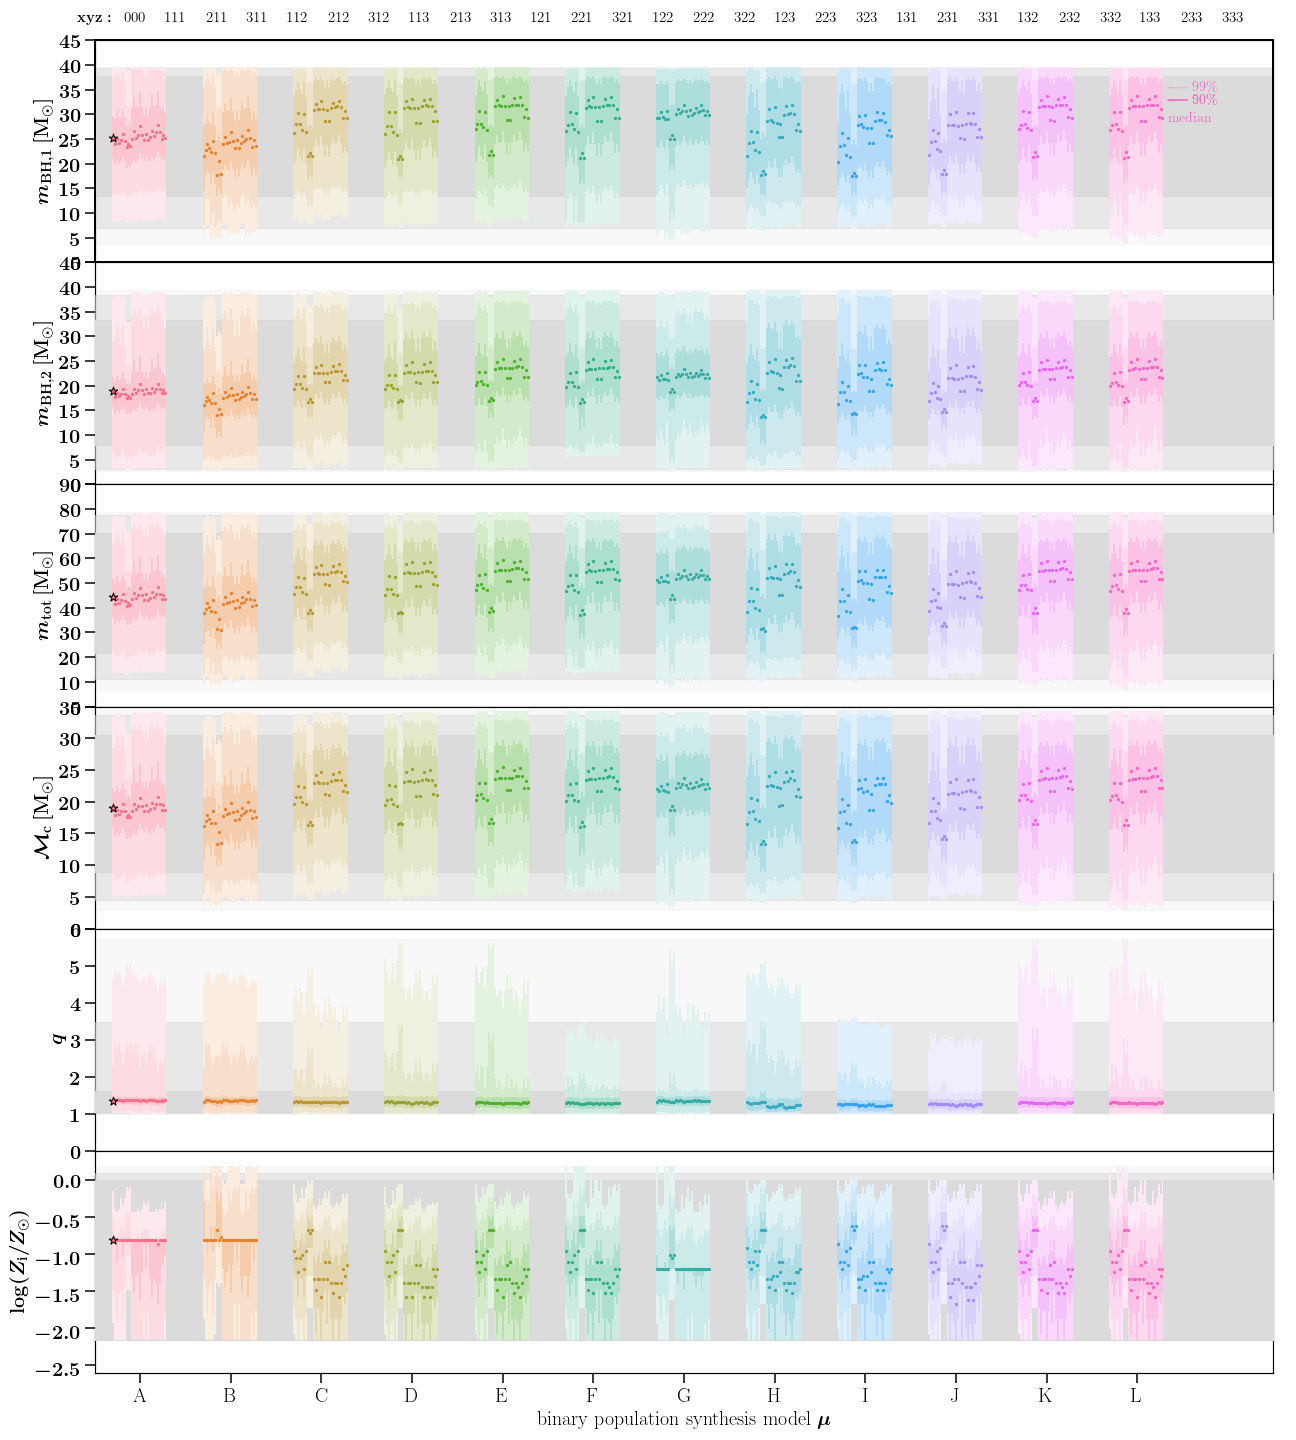
\includegraphics[width=1\textwidth]{../PlottingScripts/9_PredictedDistributions_BPS_and_MSSFR_variations/CDF_BPSandMSSFRvariations_Summary_BHBH_Z.pdf} %
\caption{BHBH}
    \label{fig:ConfidenceINtervals_BHBH}
\end{figure*}
%



For the neutron stars we see that there are a few models that move around the nasses a lot , but MSSFR also does this (especially primary) . 


%
\begin{figure*}
    \centering
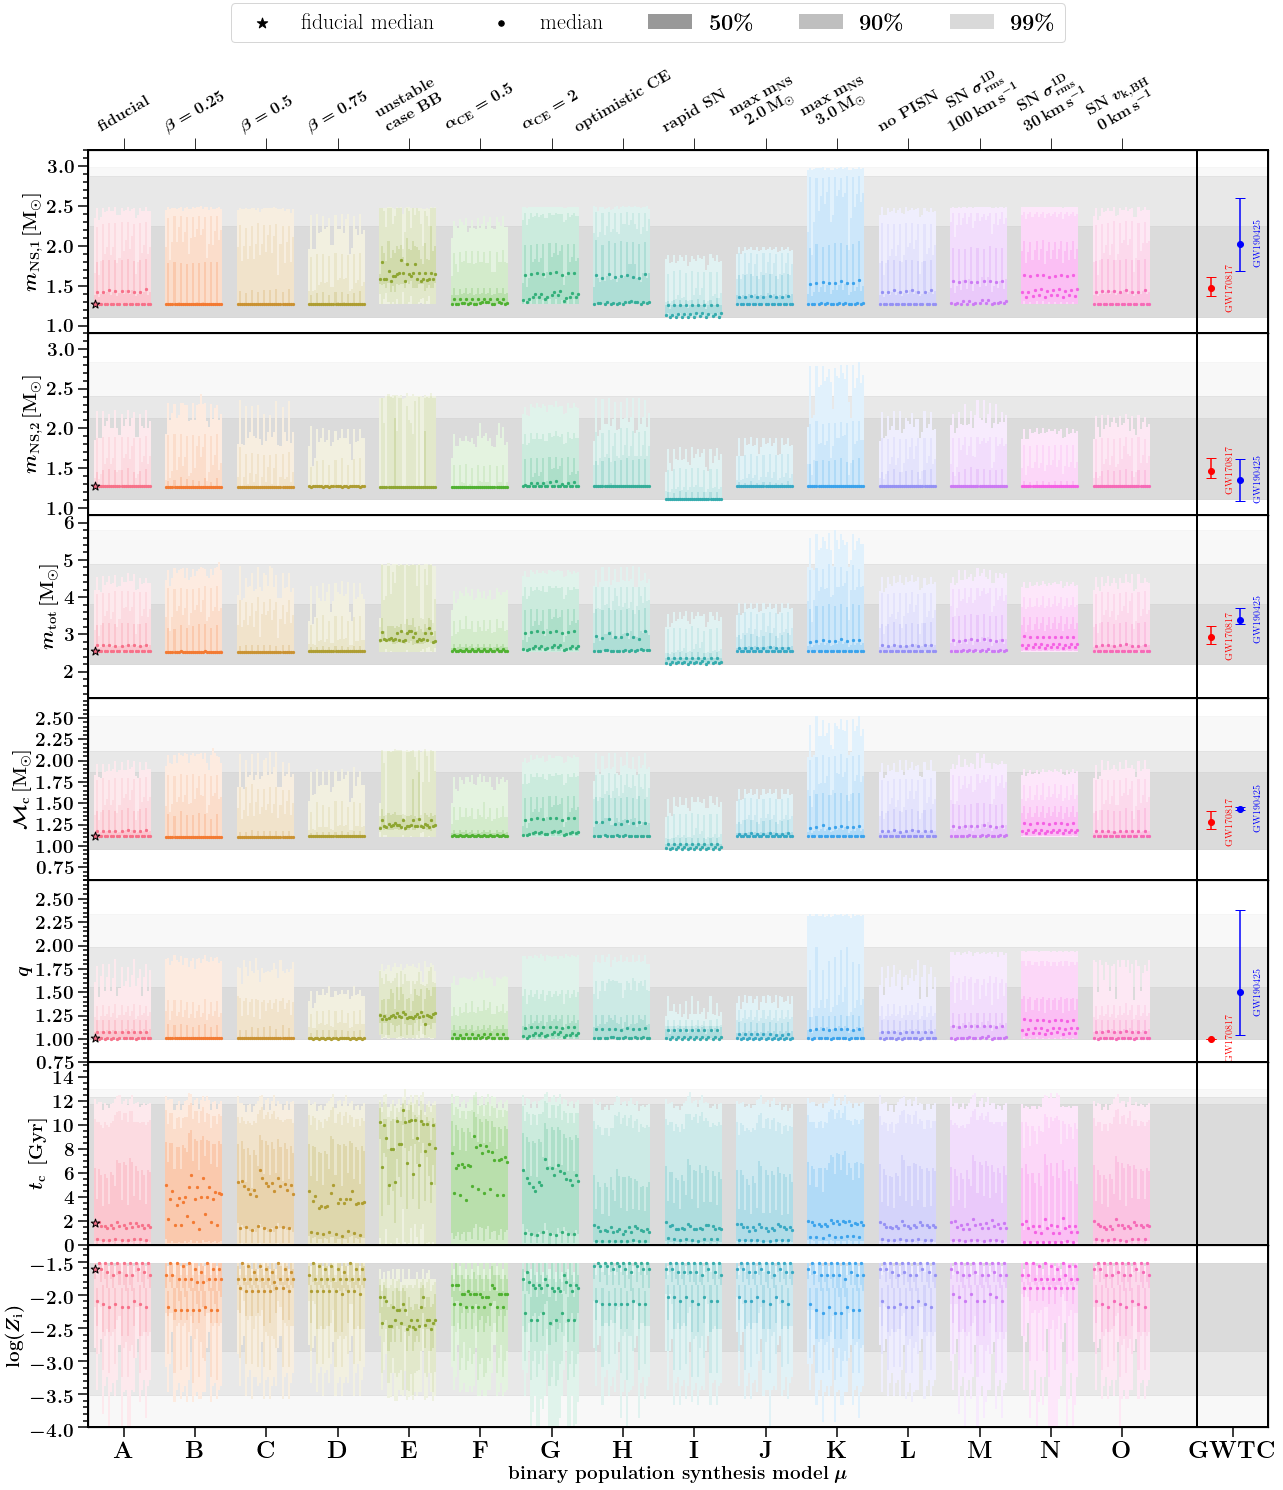
\includegraphics[width=1\textwidth]{../PlottingScripts/9_PredictedDistributions_BPS_and_MSSFR_variations/CDF_BPSandMSSFRvariations_Summary_NSNS_Z.pdf} 
\caption{ NSNS (bottom)}
    \label{fig:ConfidenceINtervals_NSNS}
\end{figure*}
%



%
\begin{figure*}
    \centering
%
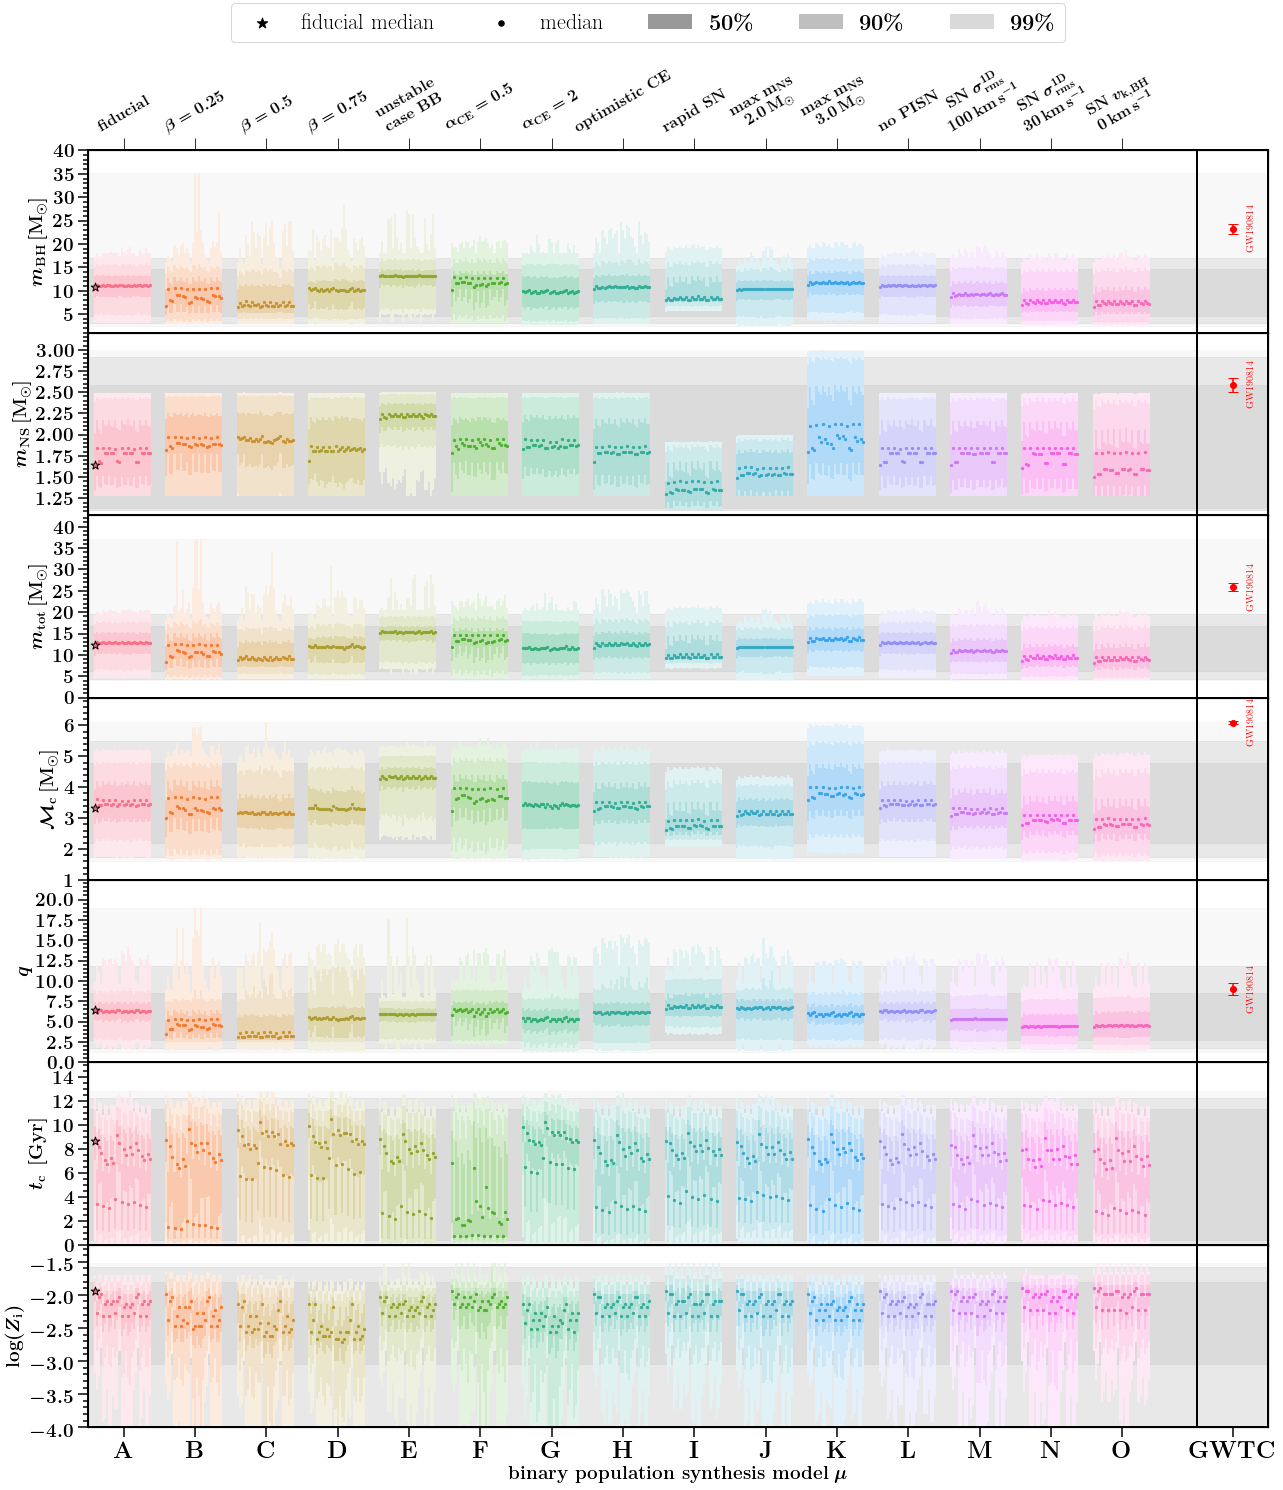
\includegraphics[width=1\textwidth]{../PlottingScripts/9_PredictedDistributions_BPS_and_MSSFR_variations/CDF_BPSandMSSFRvariations_Summary_BHNS_Z.pdf} %
%
    \caption{Confidence intervals for the predicted \bhnsSingle distributions for the variations of MSSFR and binary population synthesis models. 
    This is weighted for the detection probability for a \ac{GW} network at design sensitivity. 
    For each binary population synthesis model we show for each \ac{MSSFR} variation the median (scatter points) and $90\%$ (dark colored bar) and $99\%$  (lighter colored bar) confidence intervals.  
    In the background the greay areas show the range of the minimum and maximum 90$\%$ and 99$\%$ values over all model variations.
     The fiducial model (\mAzero) median values are shown with star symbols.   }
    %
    \label{fig:ConfidenceINtervals_BHNS}
\end{figure*}
%


\subsubsection{Fryer rapid versus delayed SN model}




%
\begin{figure*}
    \centering
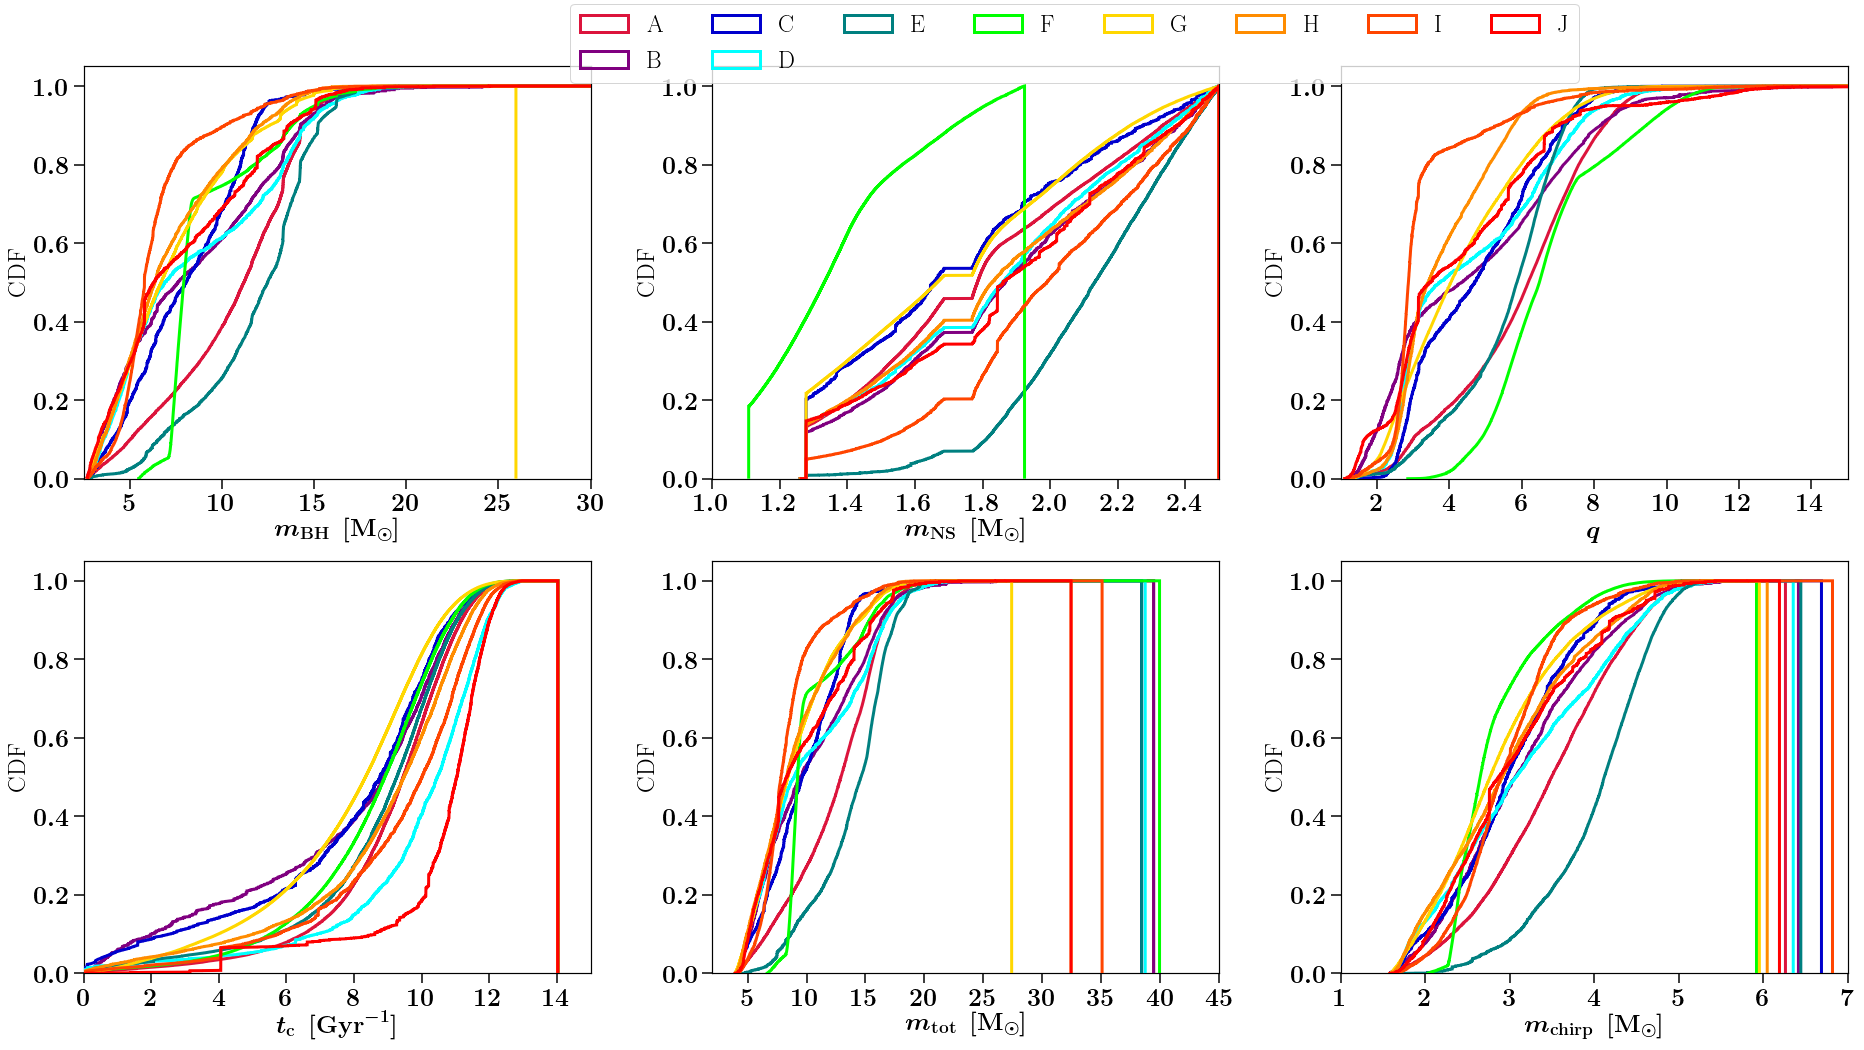
\includegraphics[width=1\textwidth]{../PlottingScripts/9_PredictedDistributions_BPS_and_MSSFR_variations/AllDistributions.png} %
    \caption{}%
    \label{fig:CDFs_BHNS_observed}
\end{figure*}
%





%
\begin{figure}
    \centering
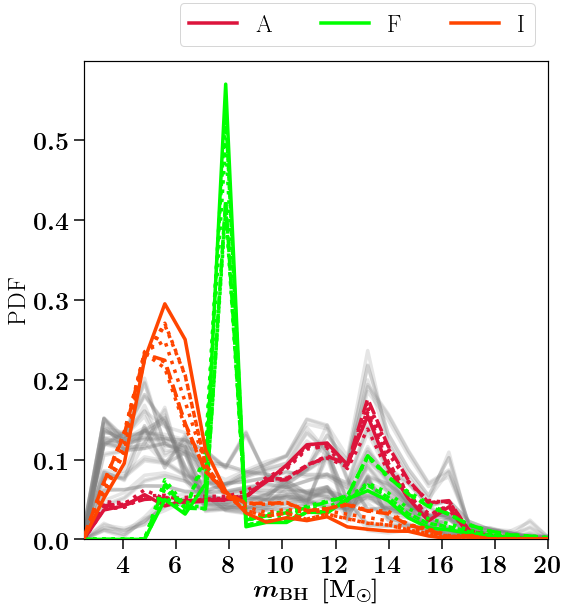
\includegraphics[width=.5\columnwidth]{../PlottingScripts/9_PredictedDistributions_BPS_and_MSSFR_variations/DistributionsModels_det_BHNS_massBH_KDE.png} %
    \caption{}%
    \label{fig:CDFs_BHNS_observed_MBH}
\end{figure}
%

%%
%\begin{figure*}
%\label{fig:CDFs_BHNS_observed}
%    \centering
%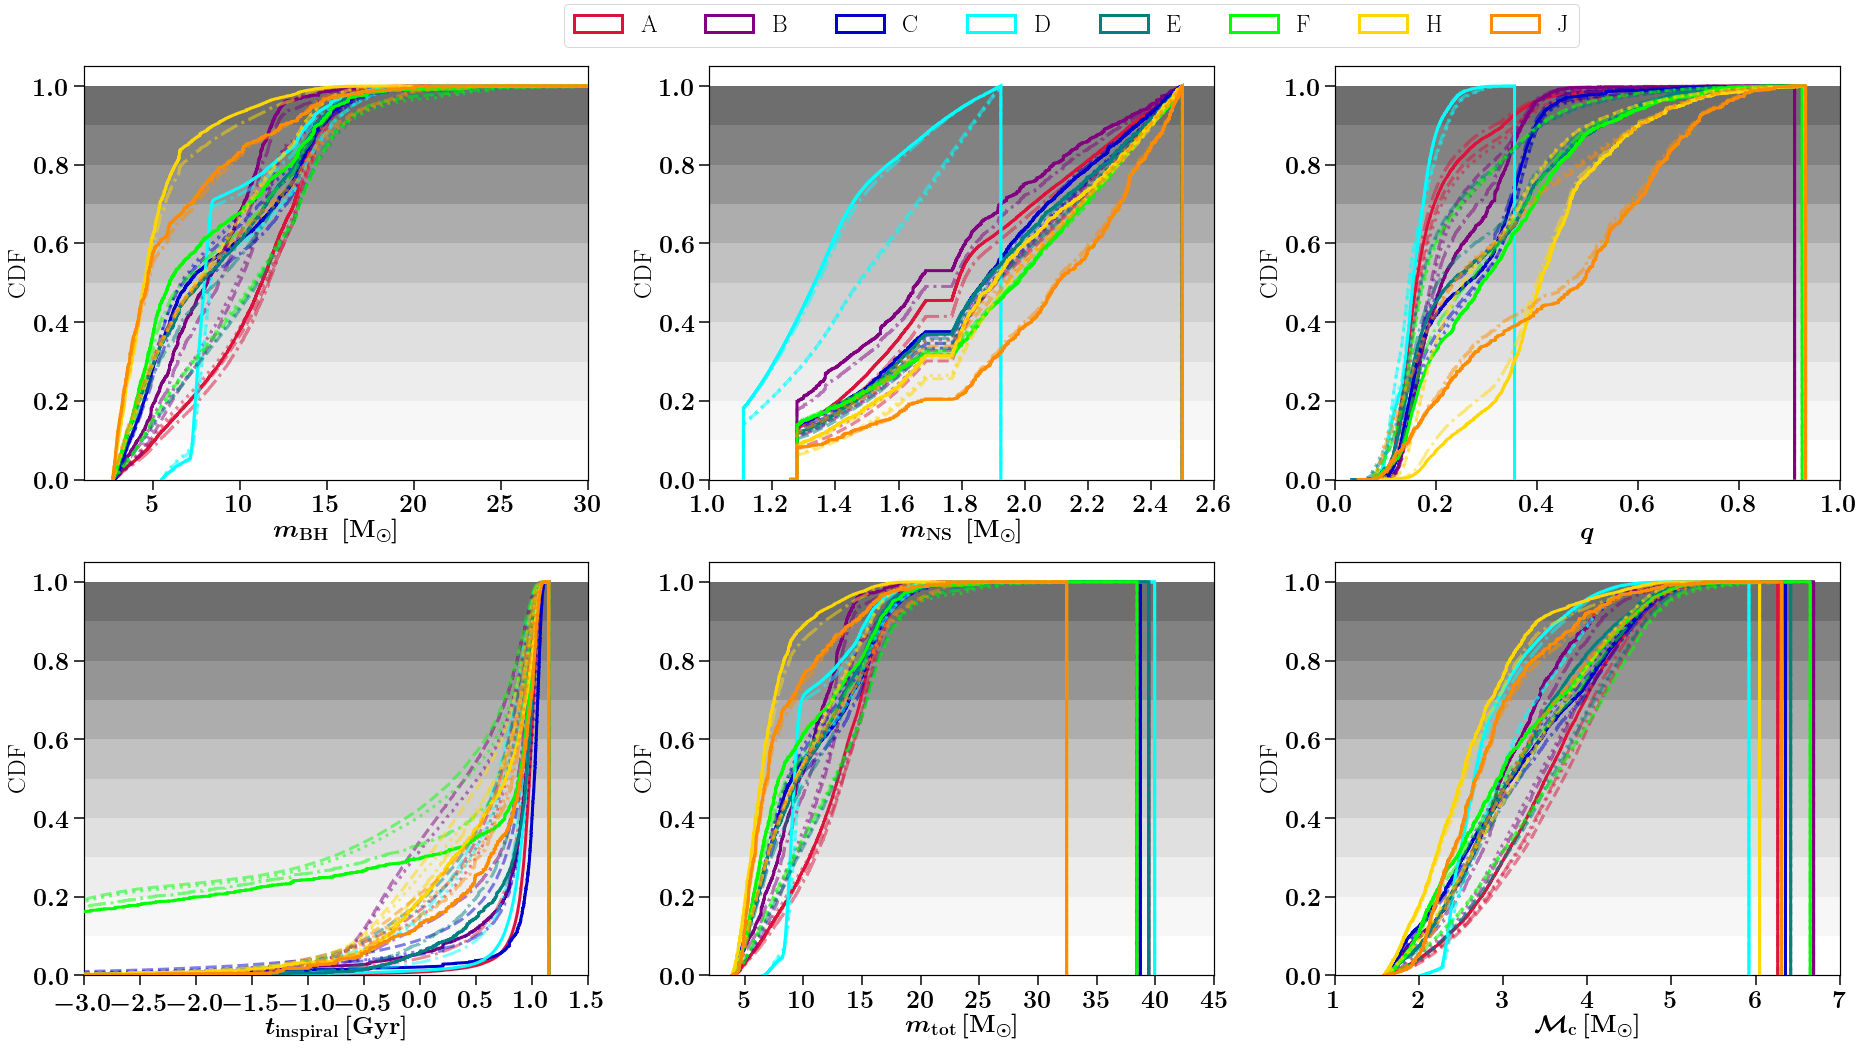
\includegraphics[width=1.0\textwidth]{../PlottingScripts/4_MSSFR_observed/DistributionsModels_observed_BHNS_CDF.pdf} %
%    \caption{}%
%\end{figure*}
%%




%
%%%
%%
%\begin{figure*}
%    \centering
%    \subfloat[NS mass ]{{\includegraphics[width=1.0\columnwidth]{../PlottingScripts/4_MSSFR_observed/mnsDistributionAtRedshiftObscombinedmodels.png} }}%
%    \qquad
%    \subfloat[BH mass ]{{\includegraphics[width=1.0\columnwidth]{../PlottingScripts/4_MSSFR_observed/mbhDistributionAtRedshiftObscombinedmodels.png} }}%
%      \qquad
%%    \caption{2 Figures side by side}%
%%
%    \centering
%    \subfloat[mass ratio]{{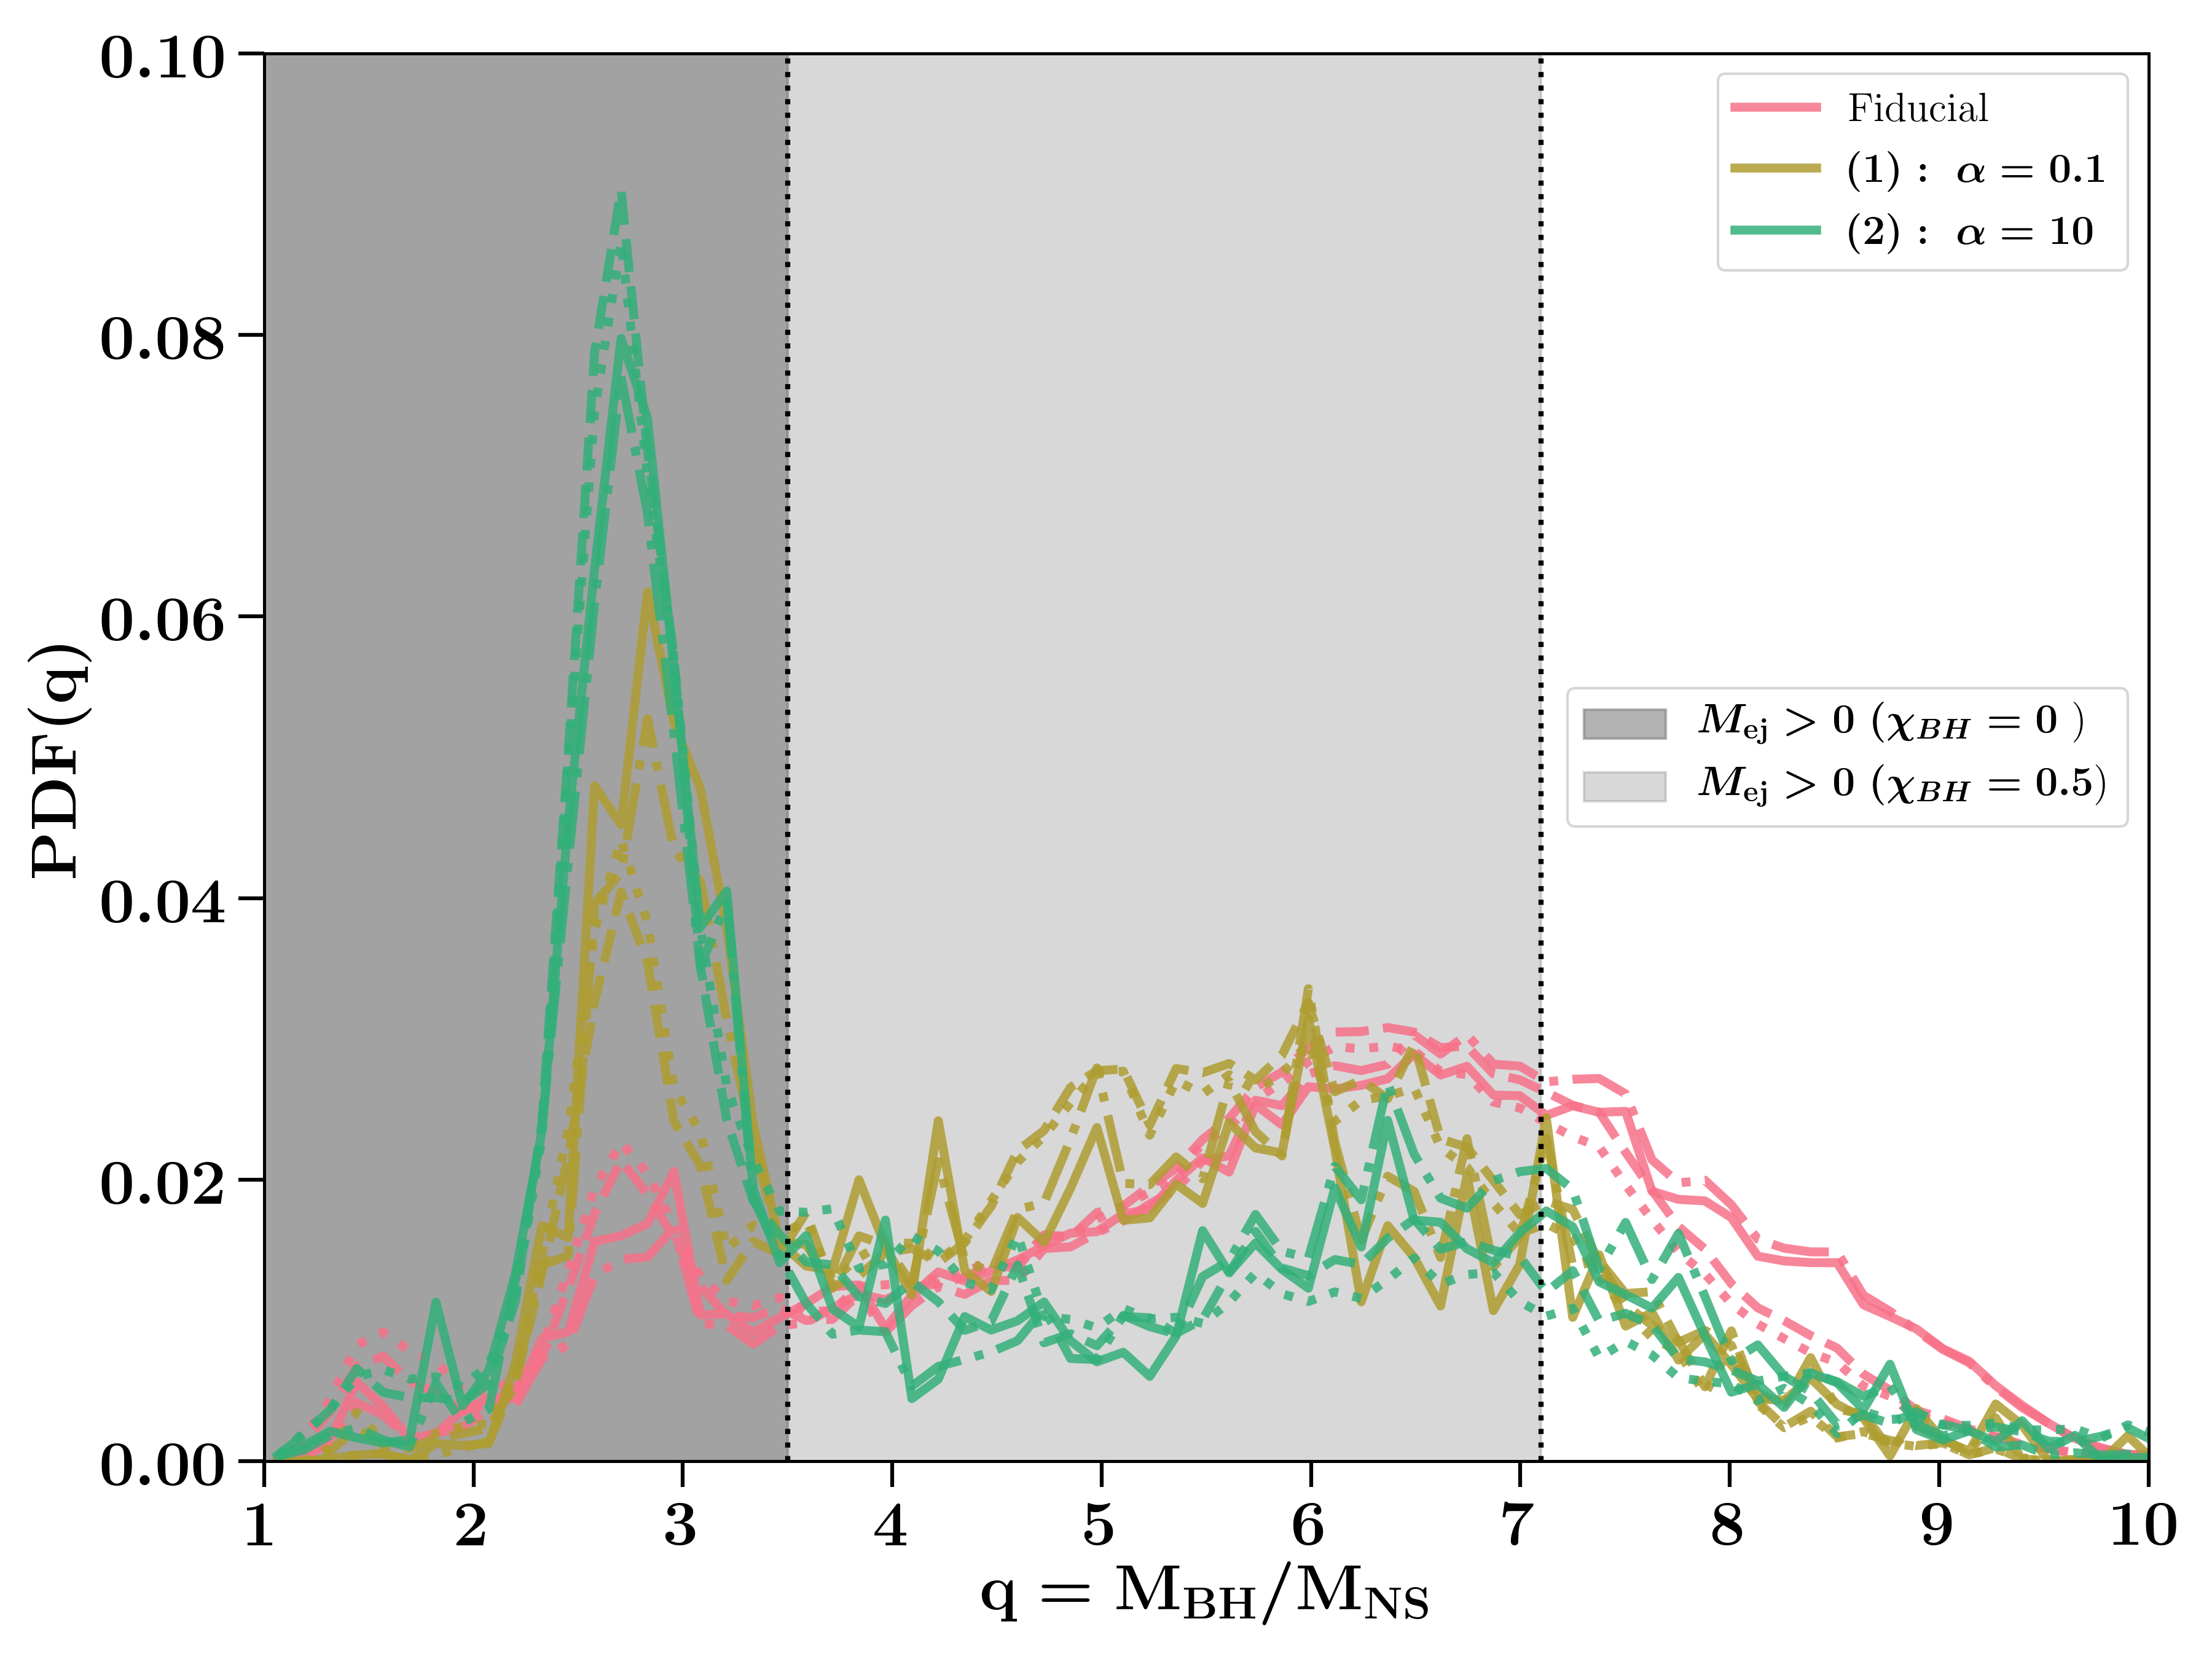
\includegraphics[width=1.0\columnwidth]{../PlottingScripts/4_MSSFR_observed/qDistributionAtRedshiftObscombinedmodels.png} }}%
%    \qquad
%    \subfloat[inspiral time]{{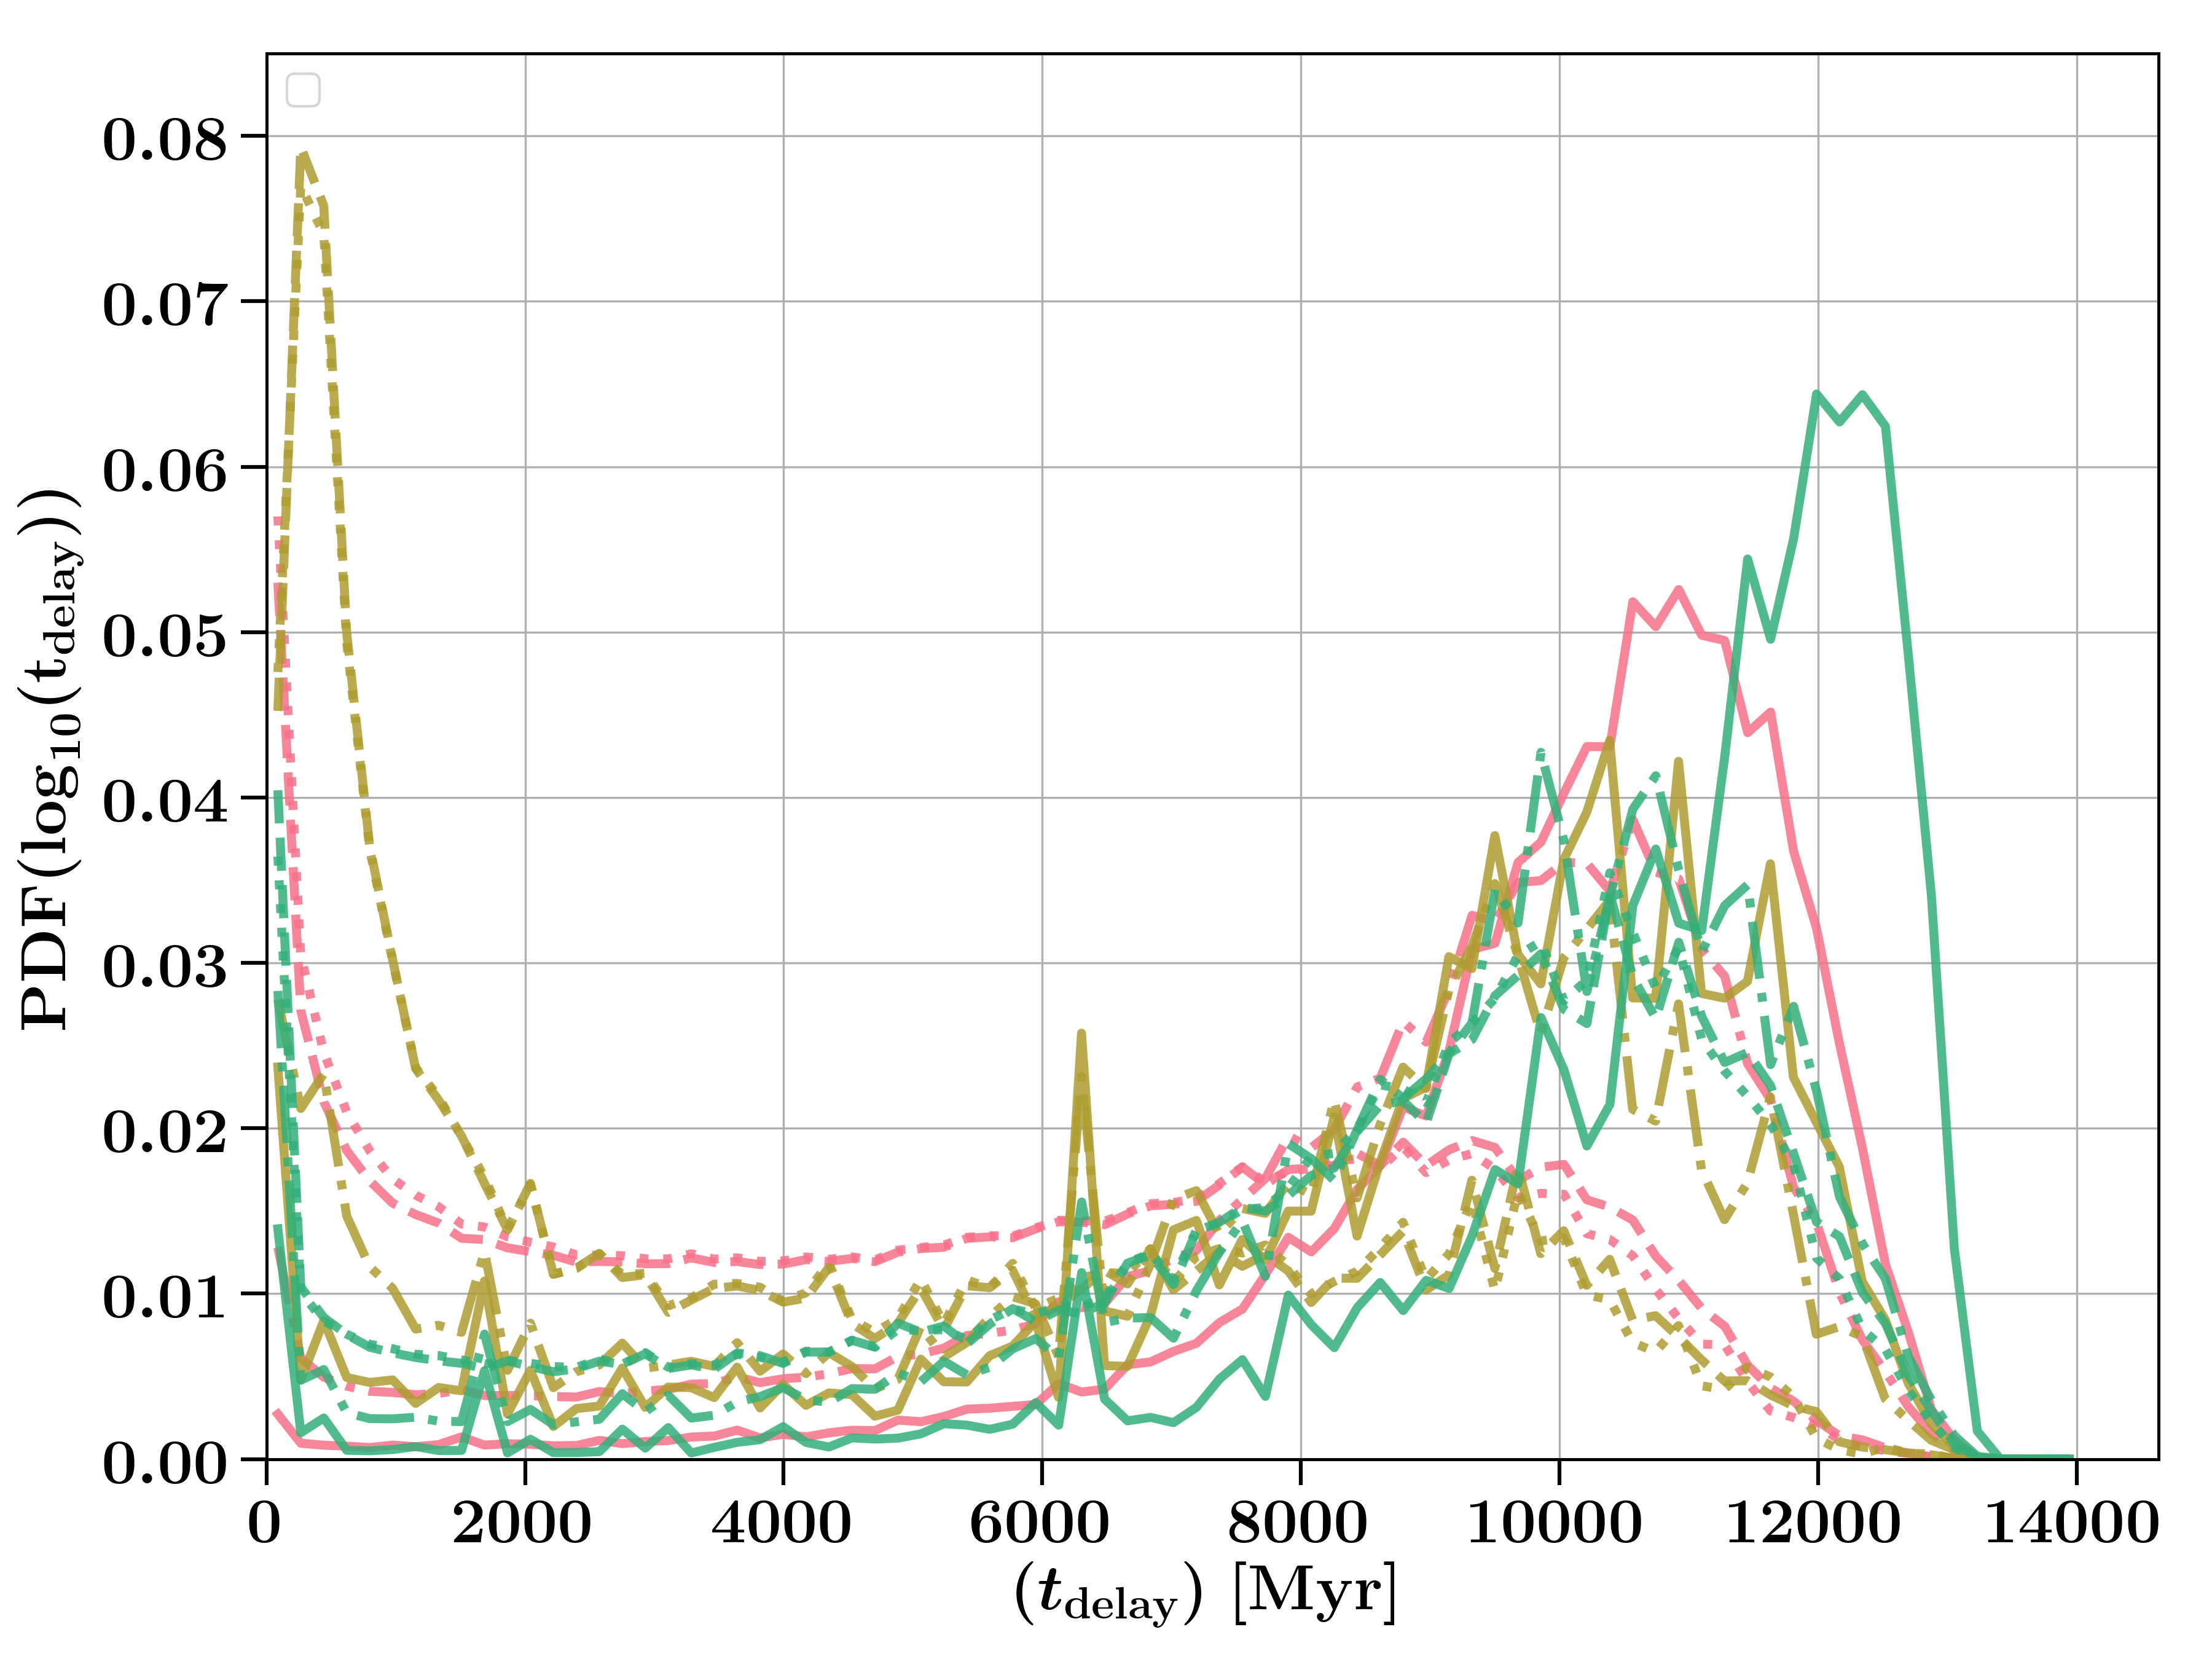
\includegraphics[width=1.0\columnwidth]{../PlottingScripts/4_MSSFR_observed/tdelayDistributionAtRedshiftObscombinedmodelsLINLIN.png} }}
%      \qquad
%%    \caption{2 Figures side by side}%
%%
%    \centering
%        \subfloat[total mass]{{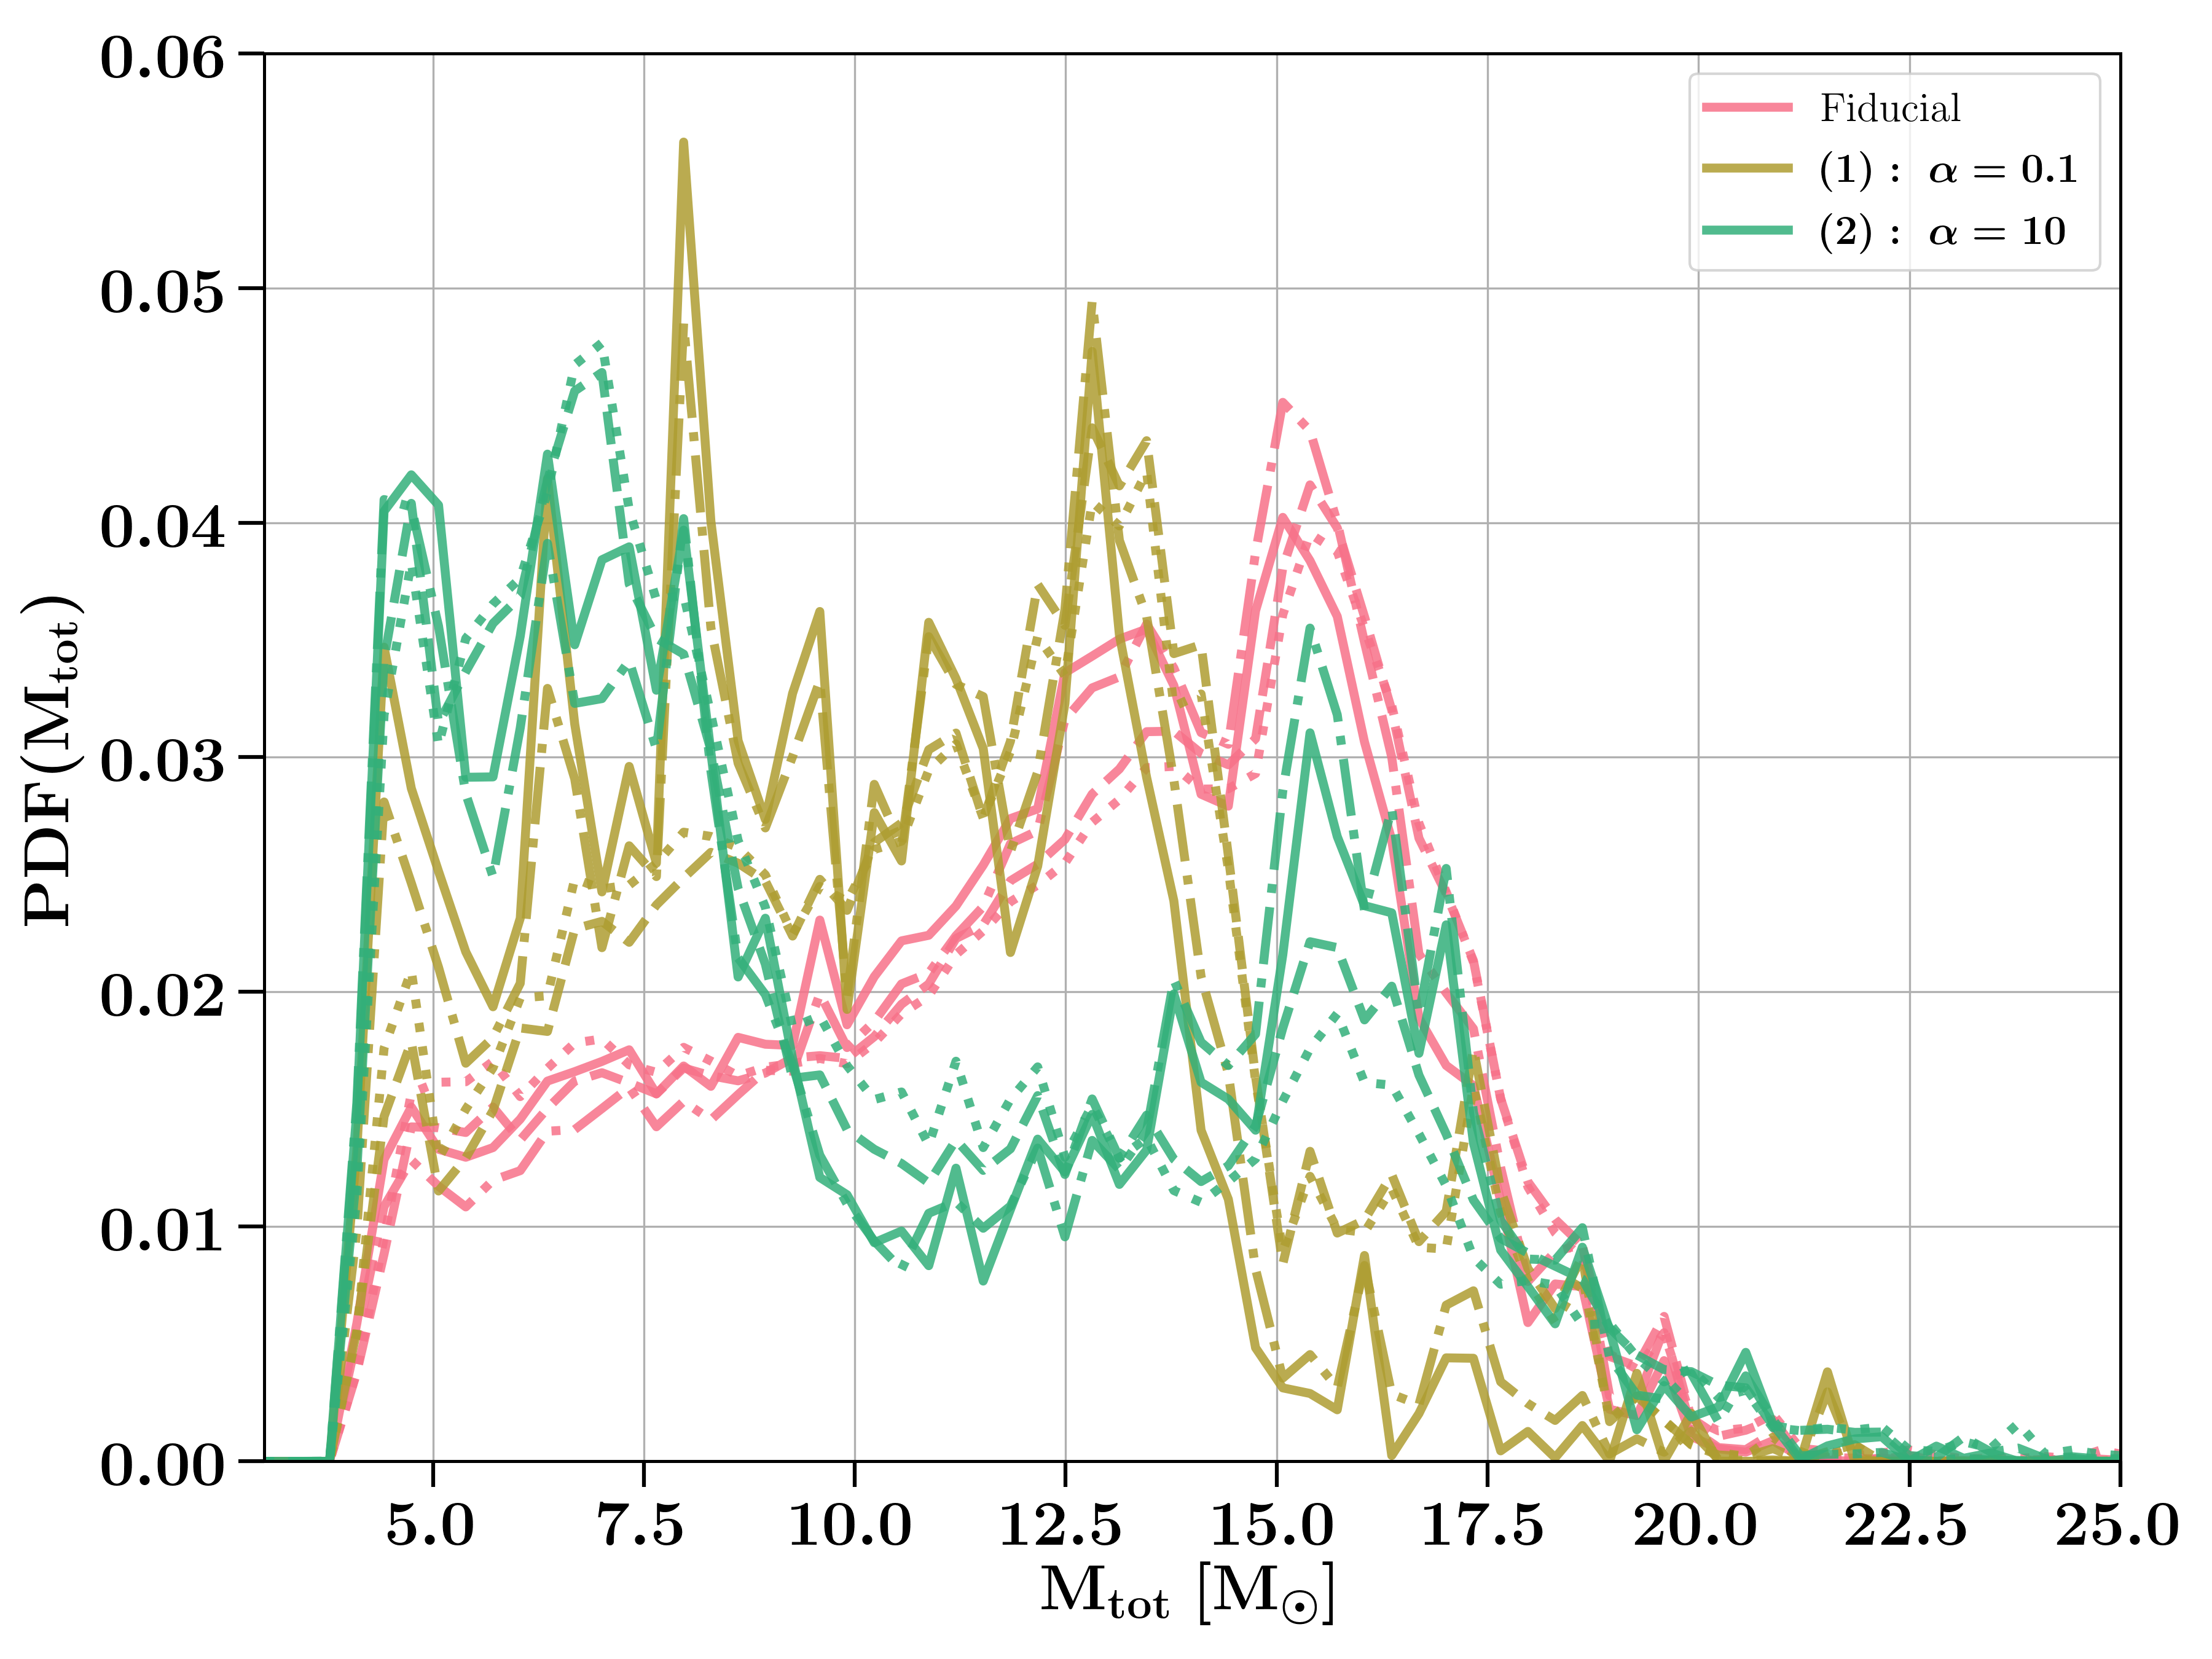
\includegraphics[width=1.0\columnwidth]{../PlottingScripts/4_MSSFR_observed/mtotDistributionAtRedshiftObscombinedmodels.png} }}%
%        \qquad
%    \subfloat[chirp mass]{{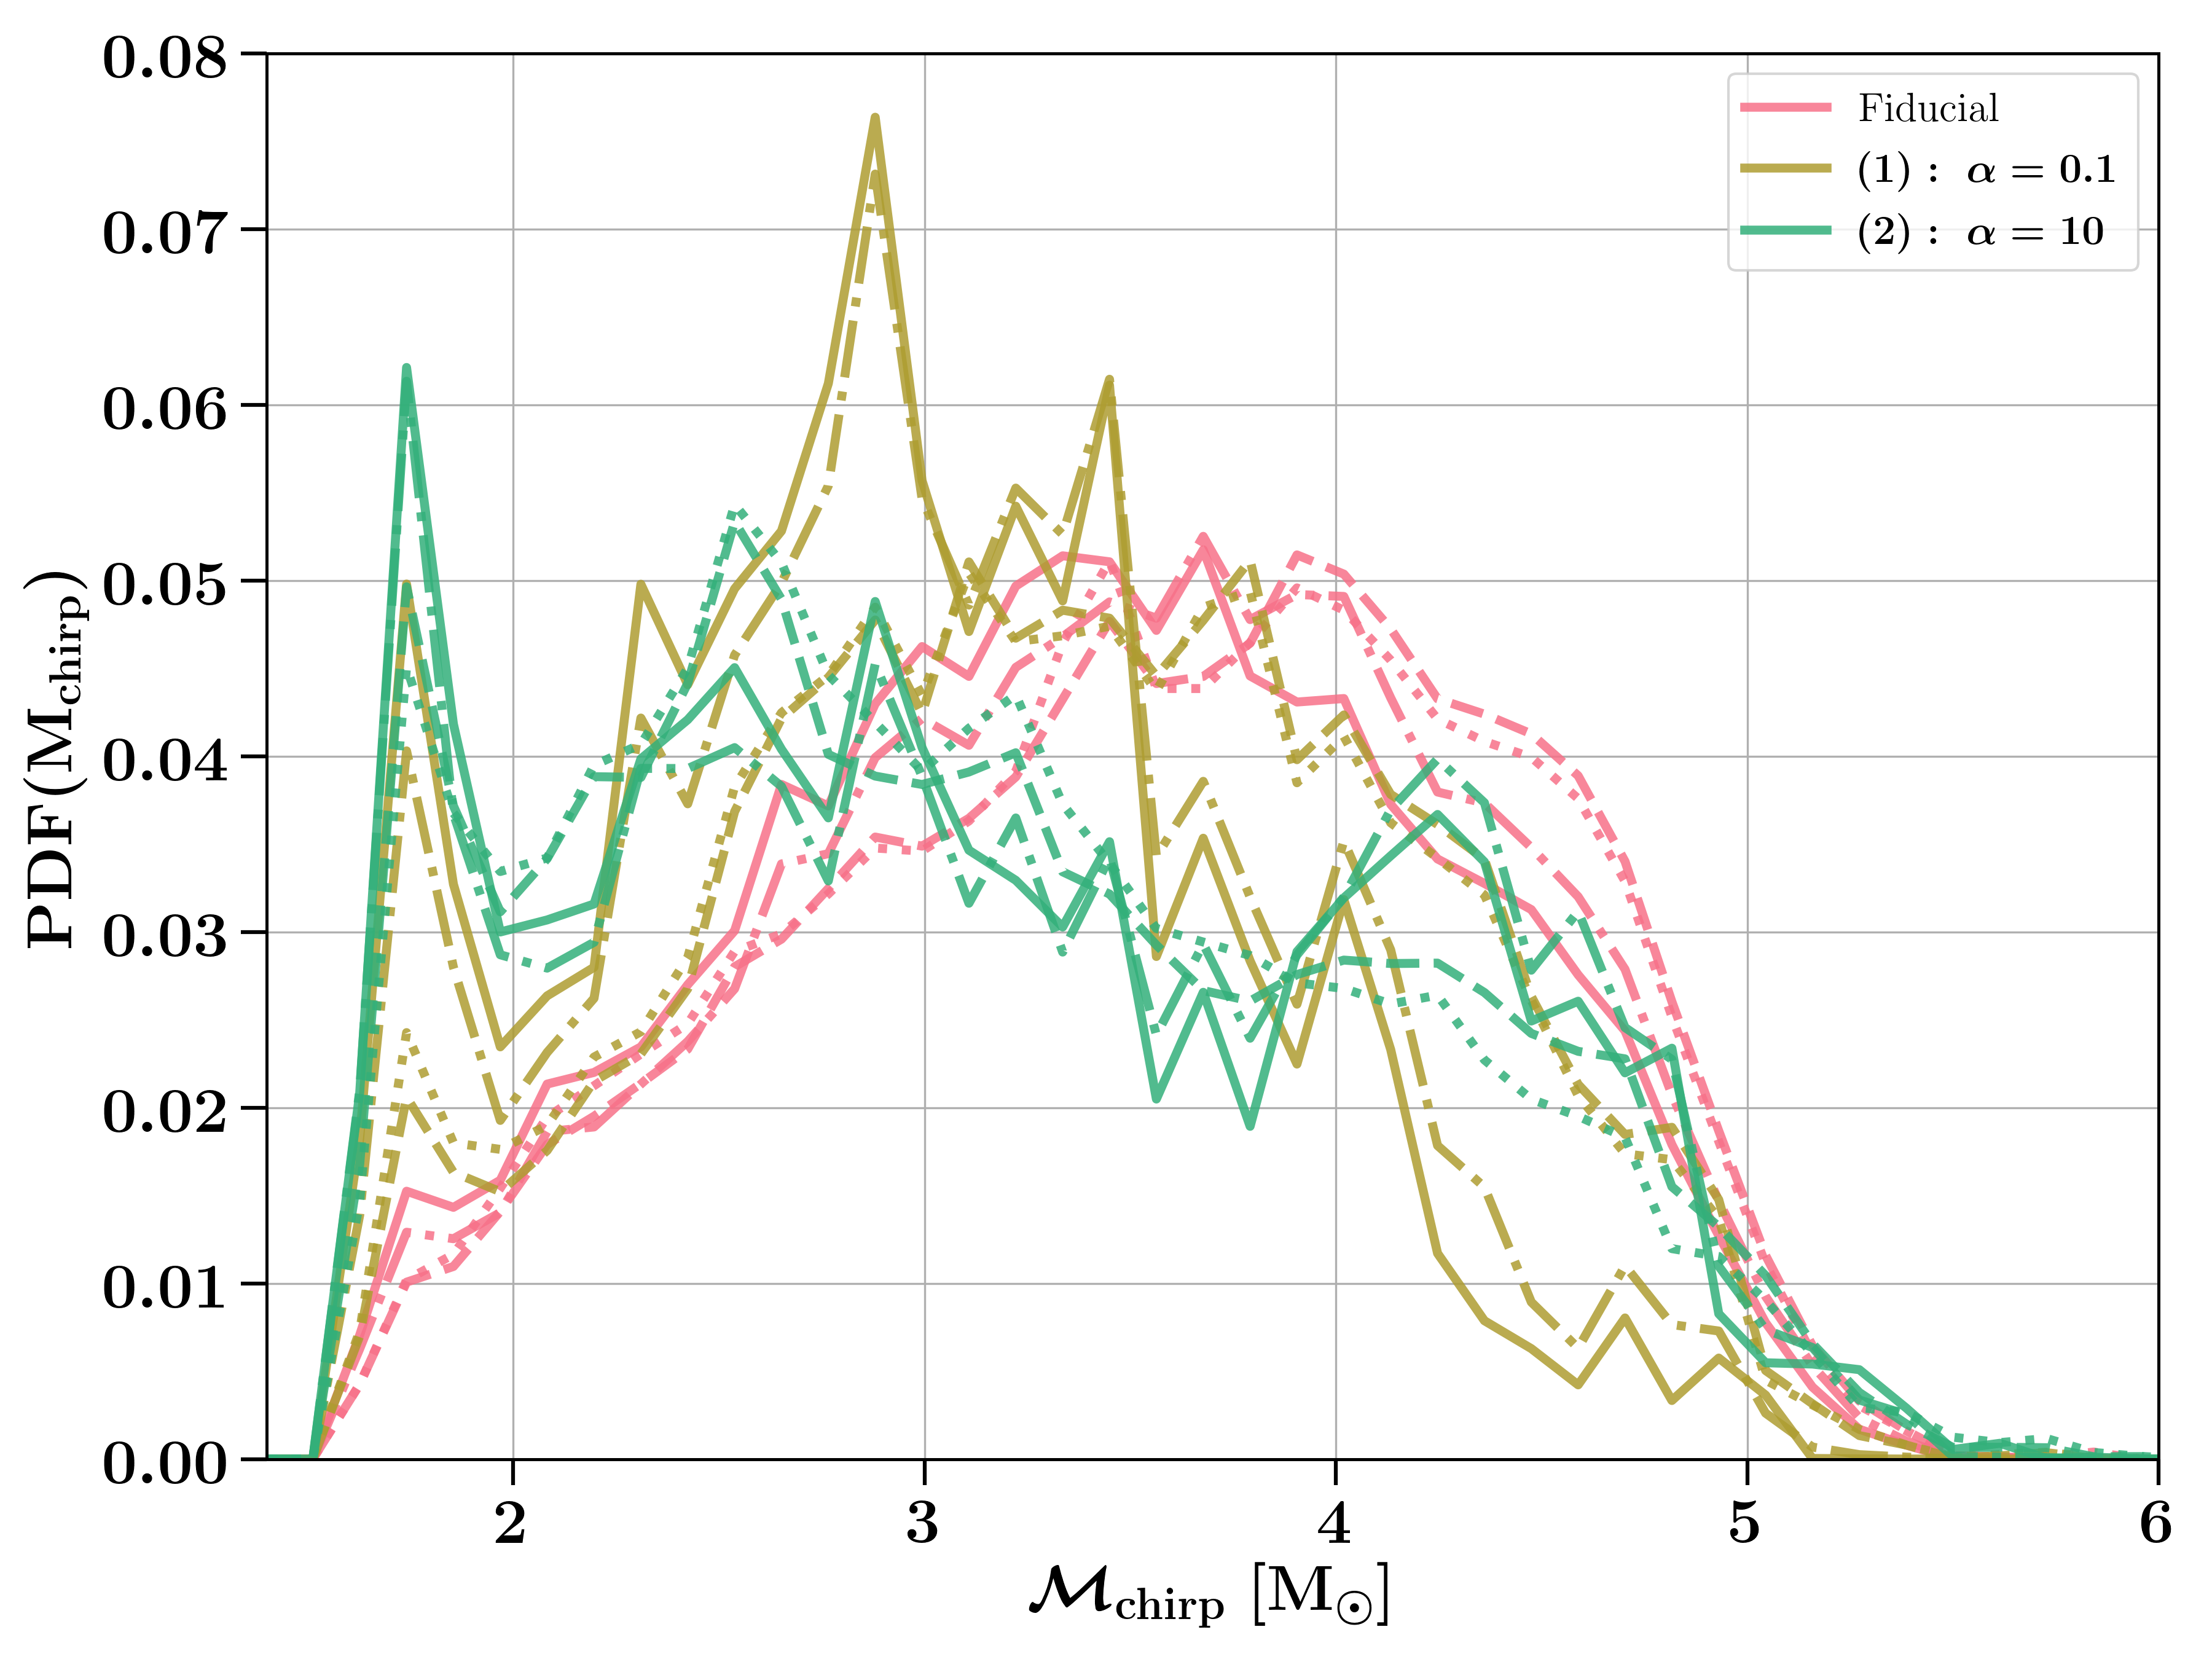
\includegraphics[width=1.0\columnwidth]{../PlottingScripts/4_MSSFR_observed/mchirpDistributionAtRedshiftObscombinedmodels.png} }}%
%    \qquad%
%    \caption{add caption }%
%\end{figure*}
%%
%





%%
%\begin{figure}
%    \centering
%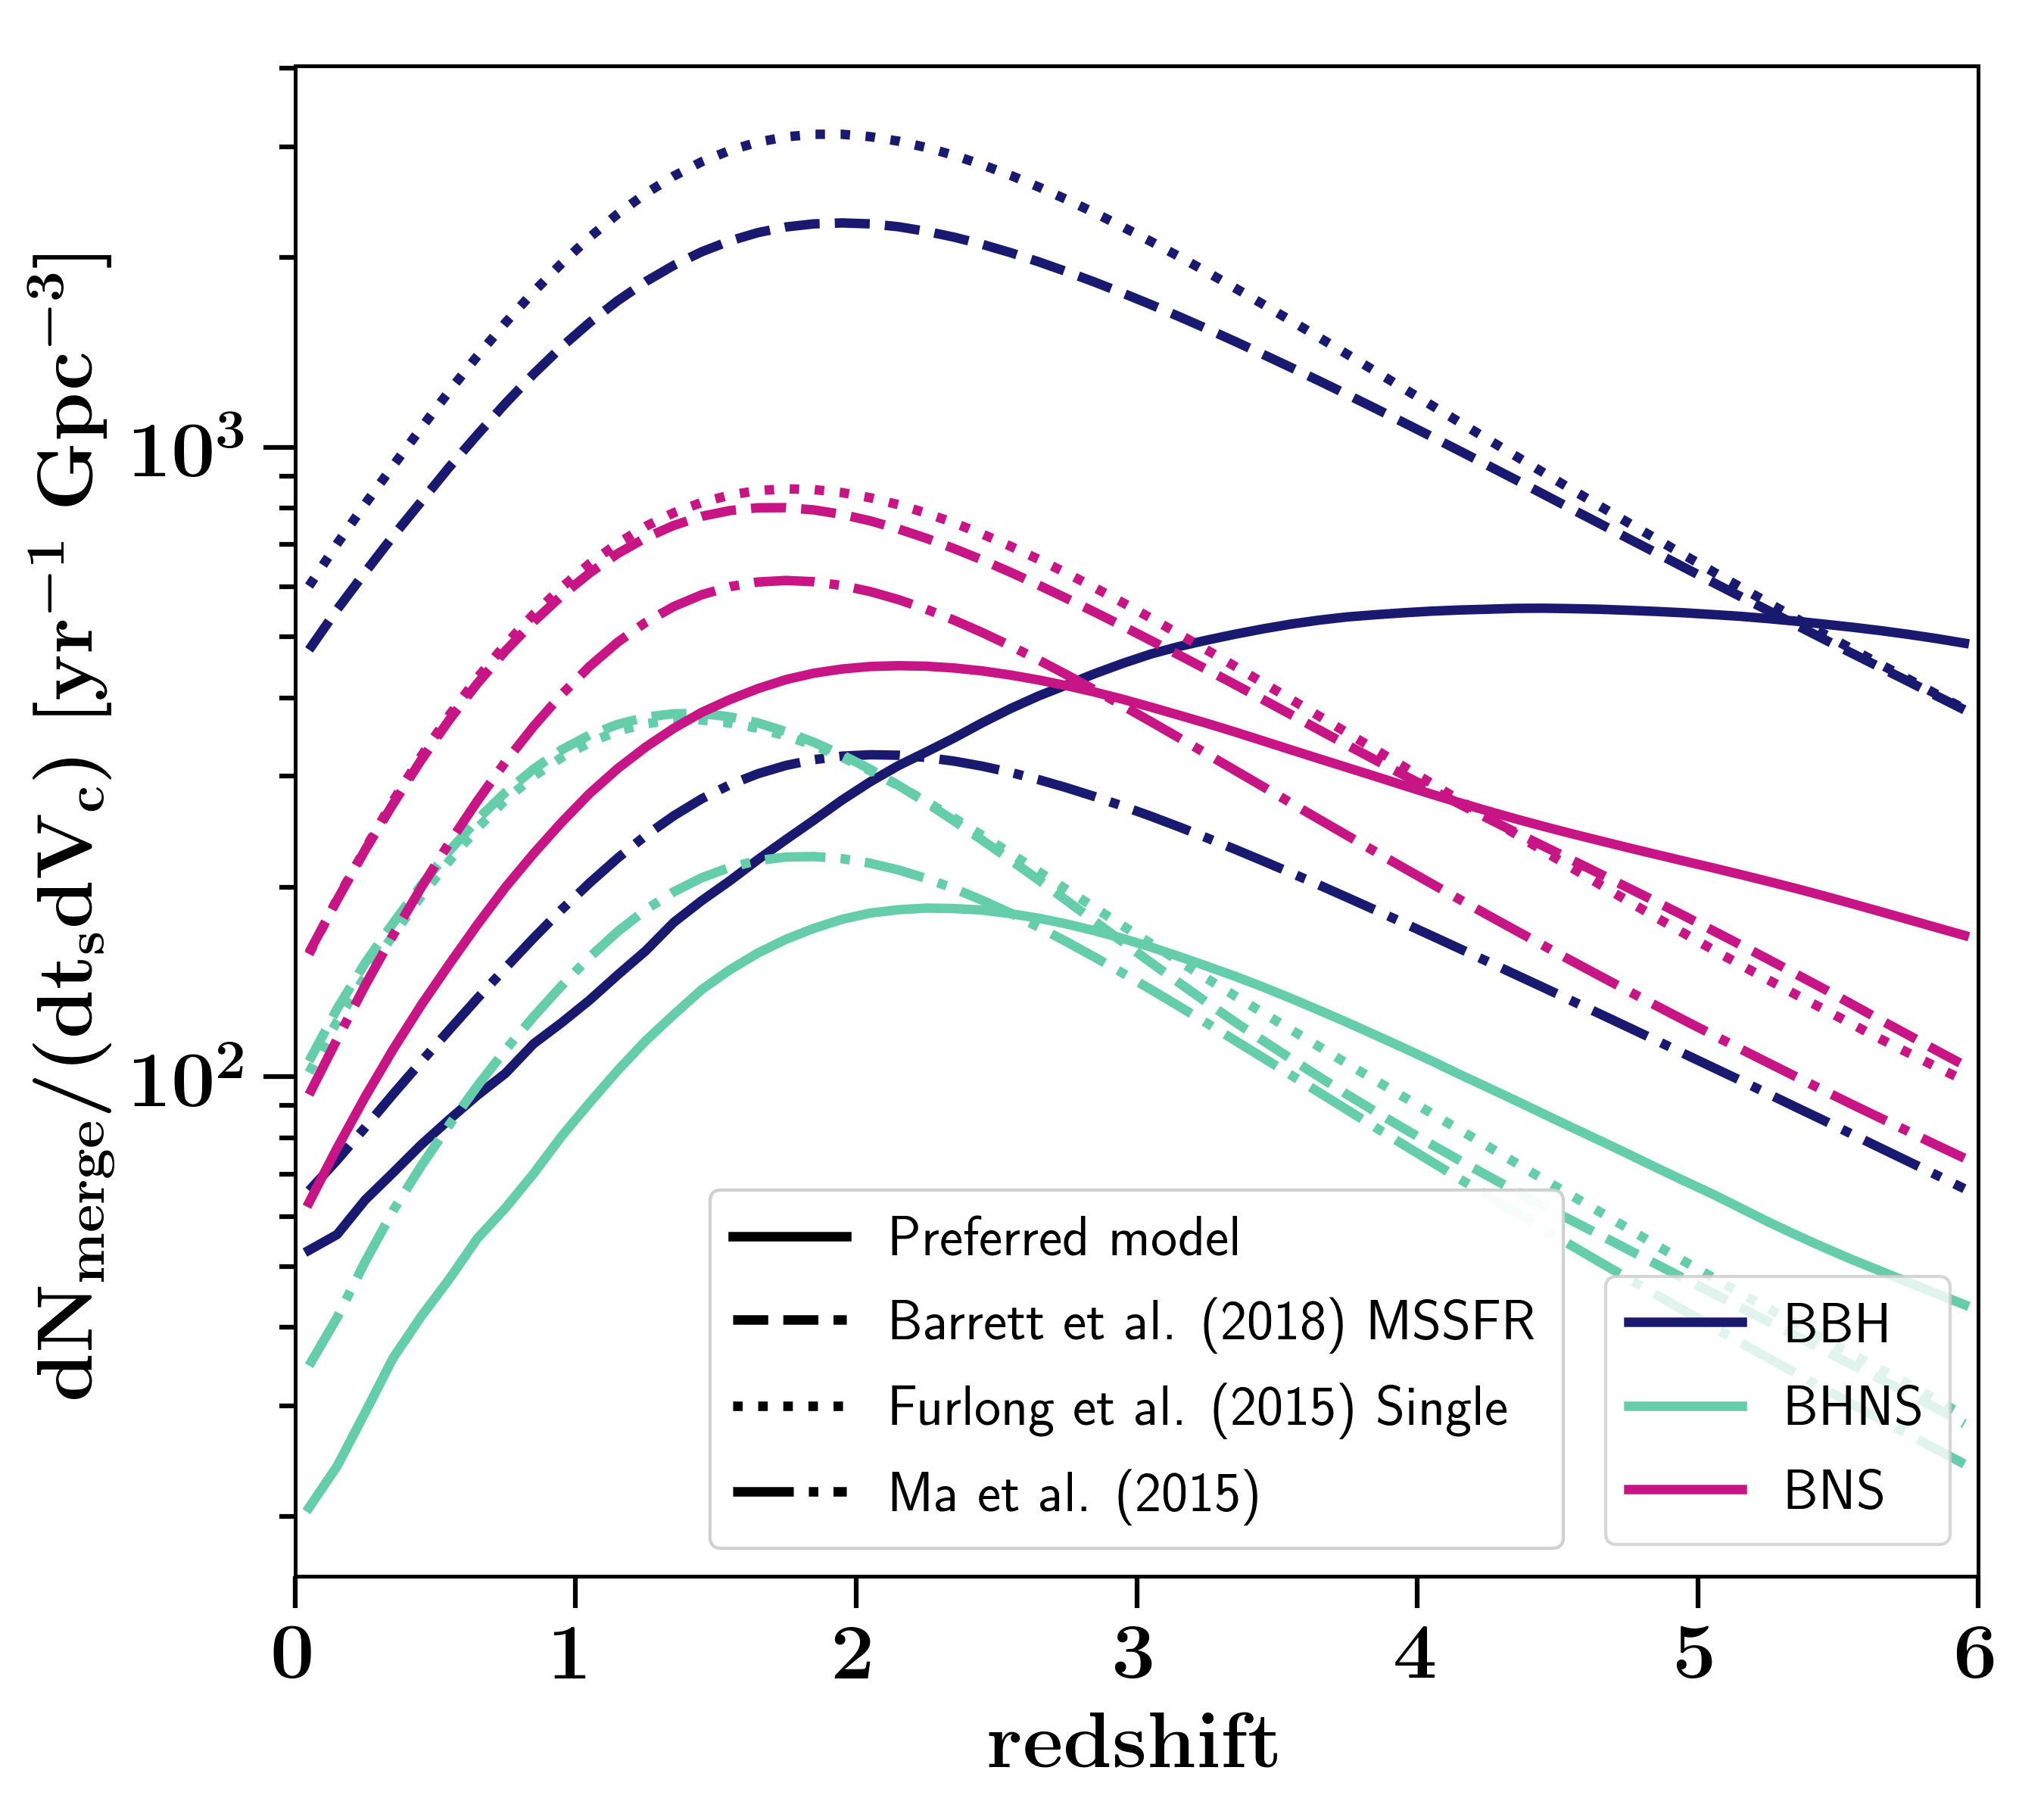
\includegraphics[width=1.0\columnwidth]{../PlottingScripts/5_DCOPerRedshift/TotalMergerRateRedshift.png} %
%
%\end{figure}
%%
%
%


%\begin{figure}
%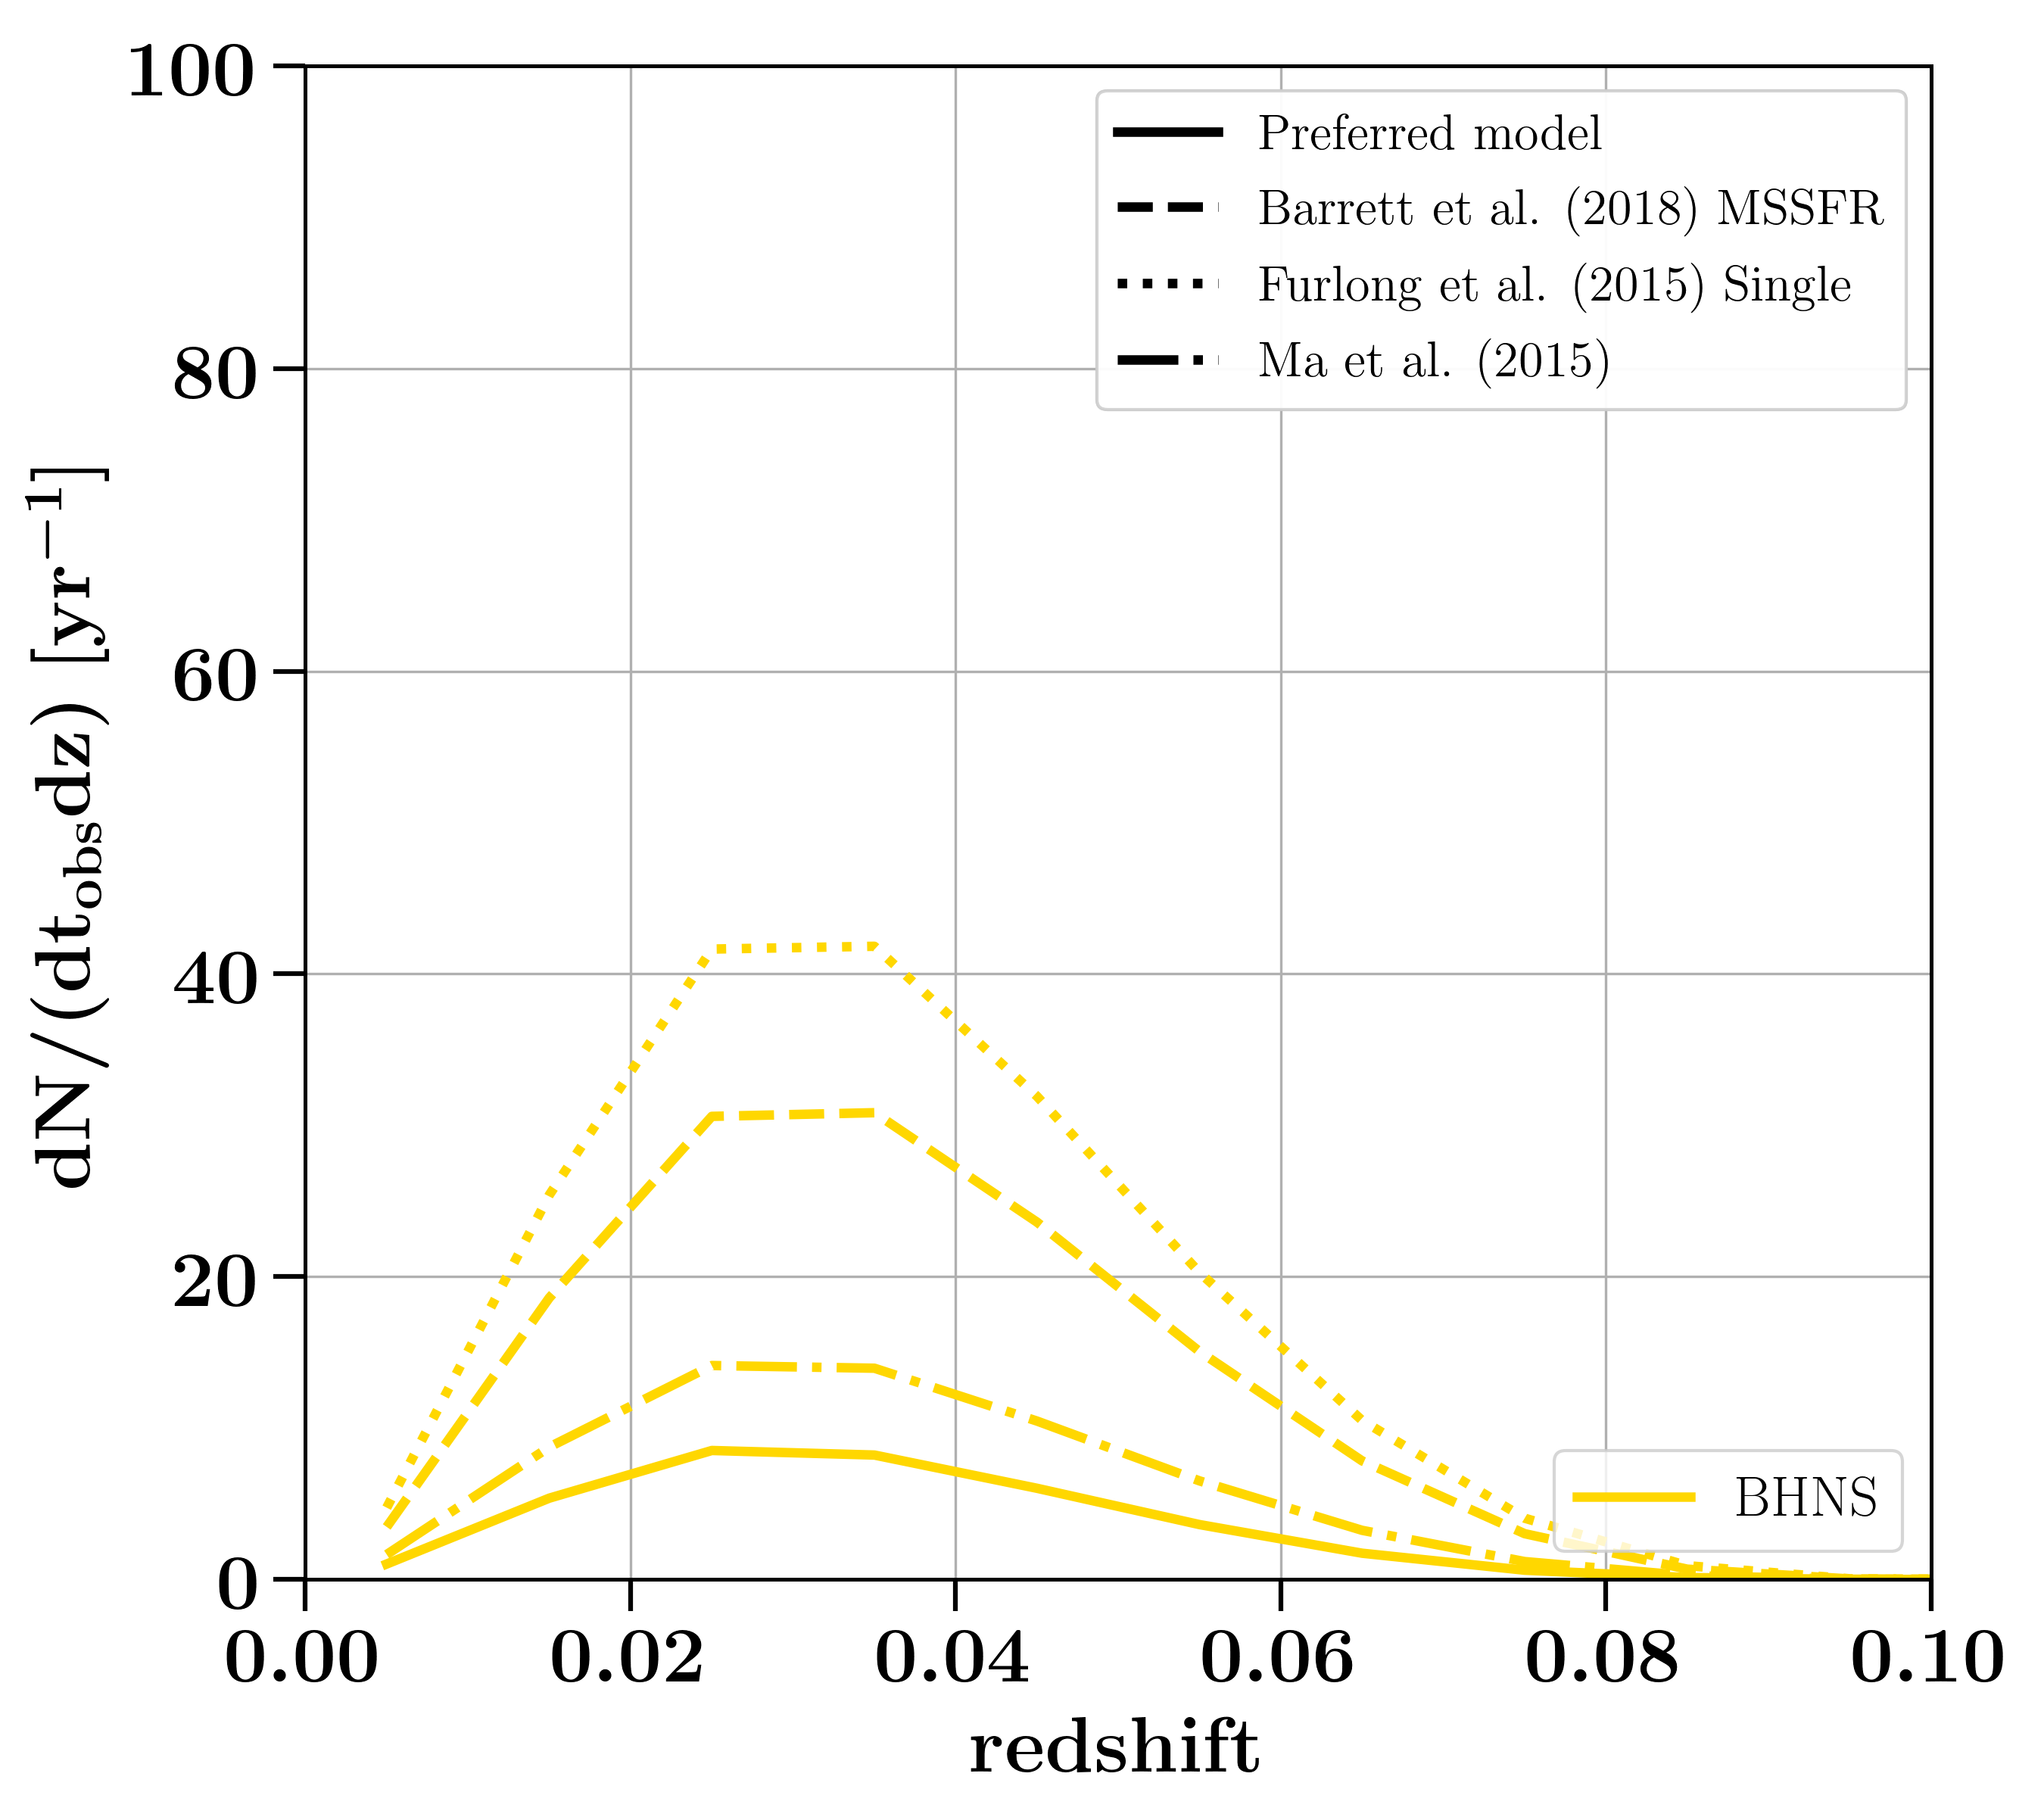
\includegraphics[width=1\columnwidth]{../PlottingScripts/4_MSSFR_observed/TotalMergerRateRedshiftObs-BHNS.png}
%   \caption{redshifts at which we will see \bhnsSingle mergers with LVK \ac{GW} network
%   }
%  \label{fig:BHNS_DCO_LVK-redshift}
%\end{figure}
%%

%\begin{figure}
%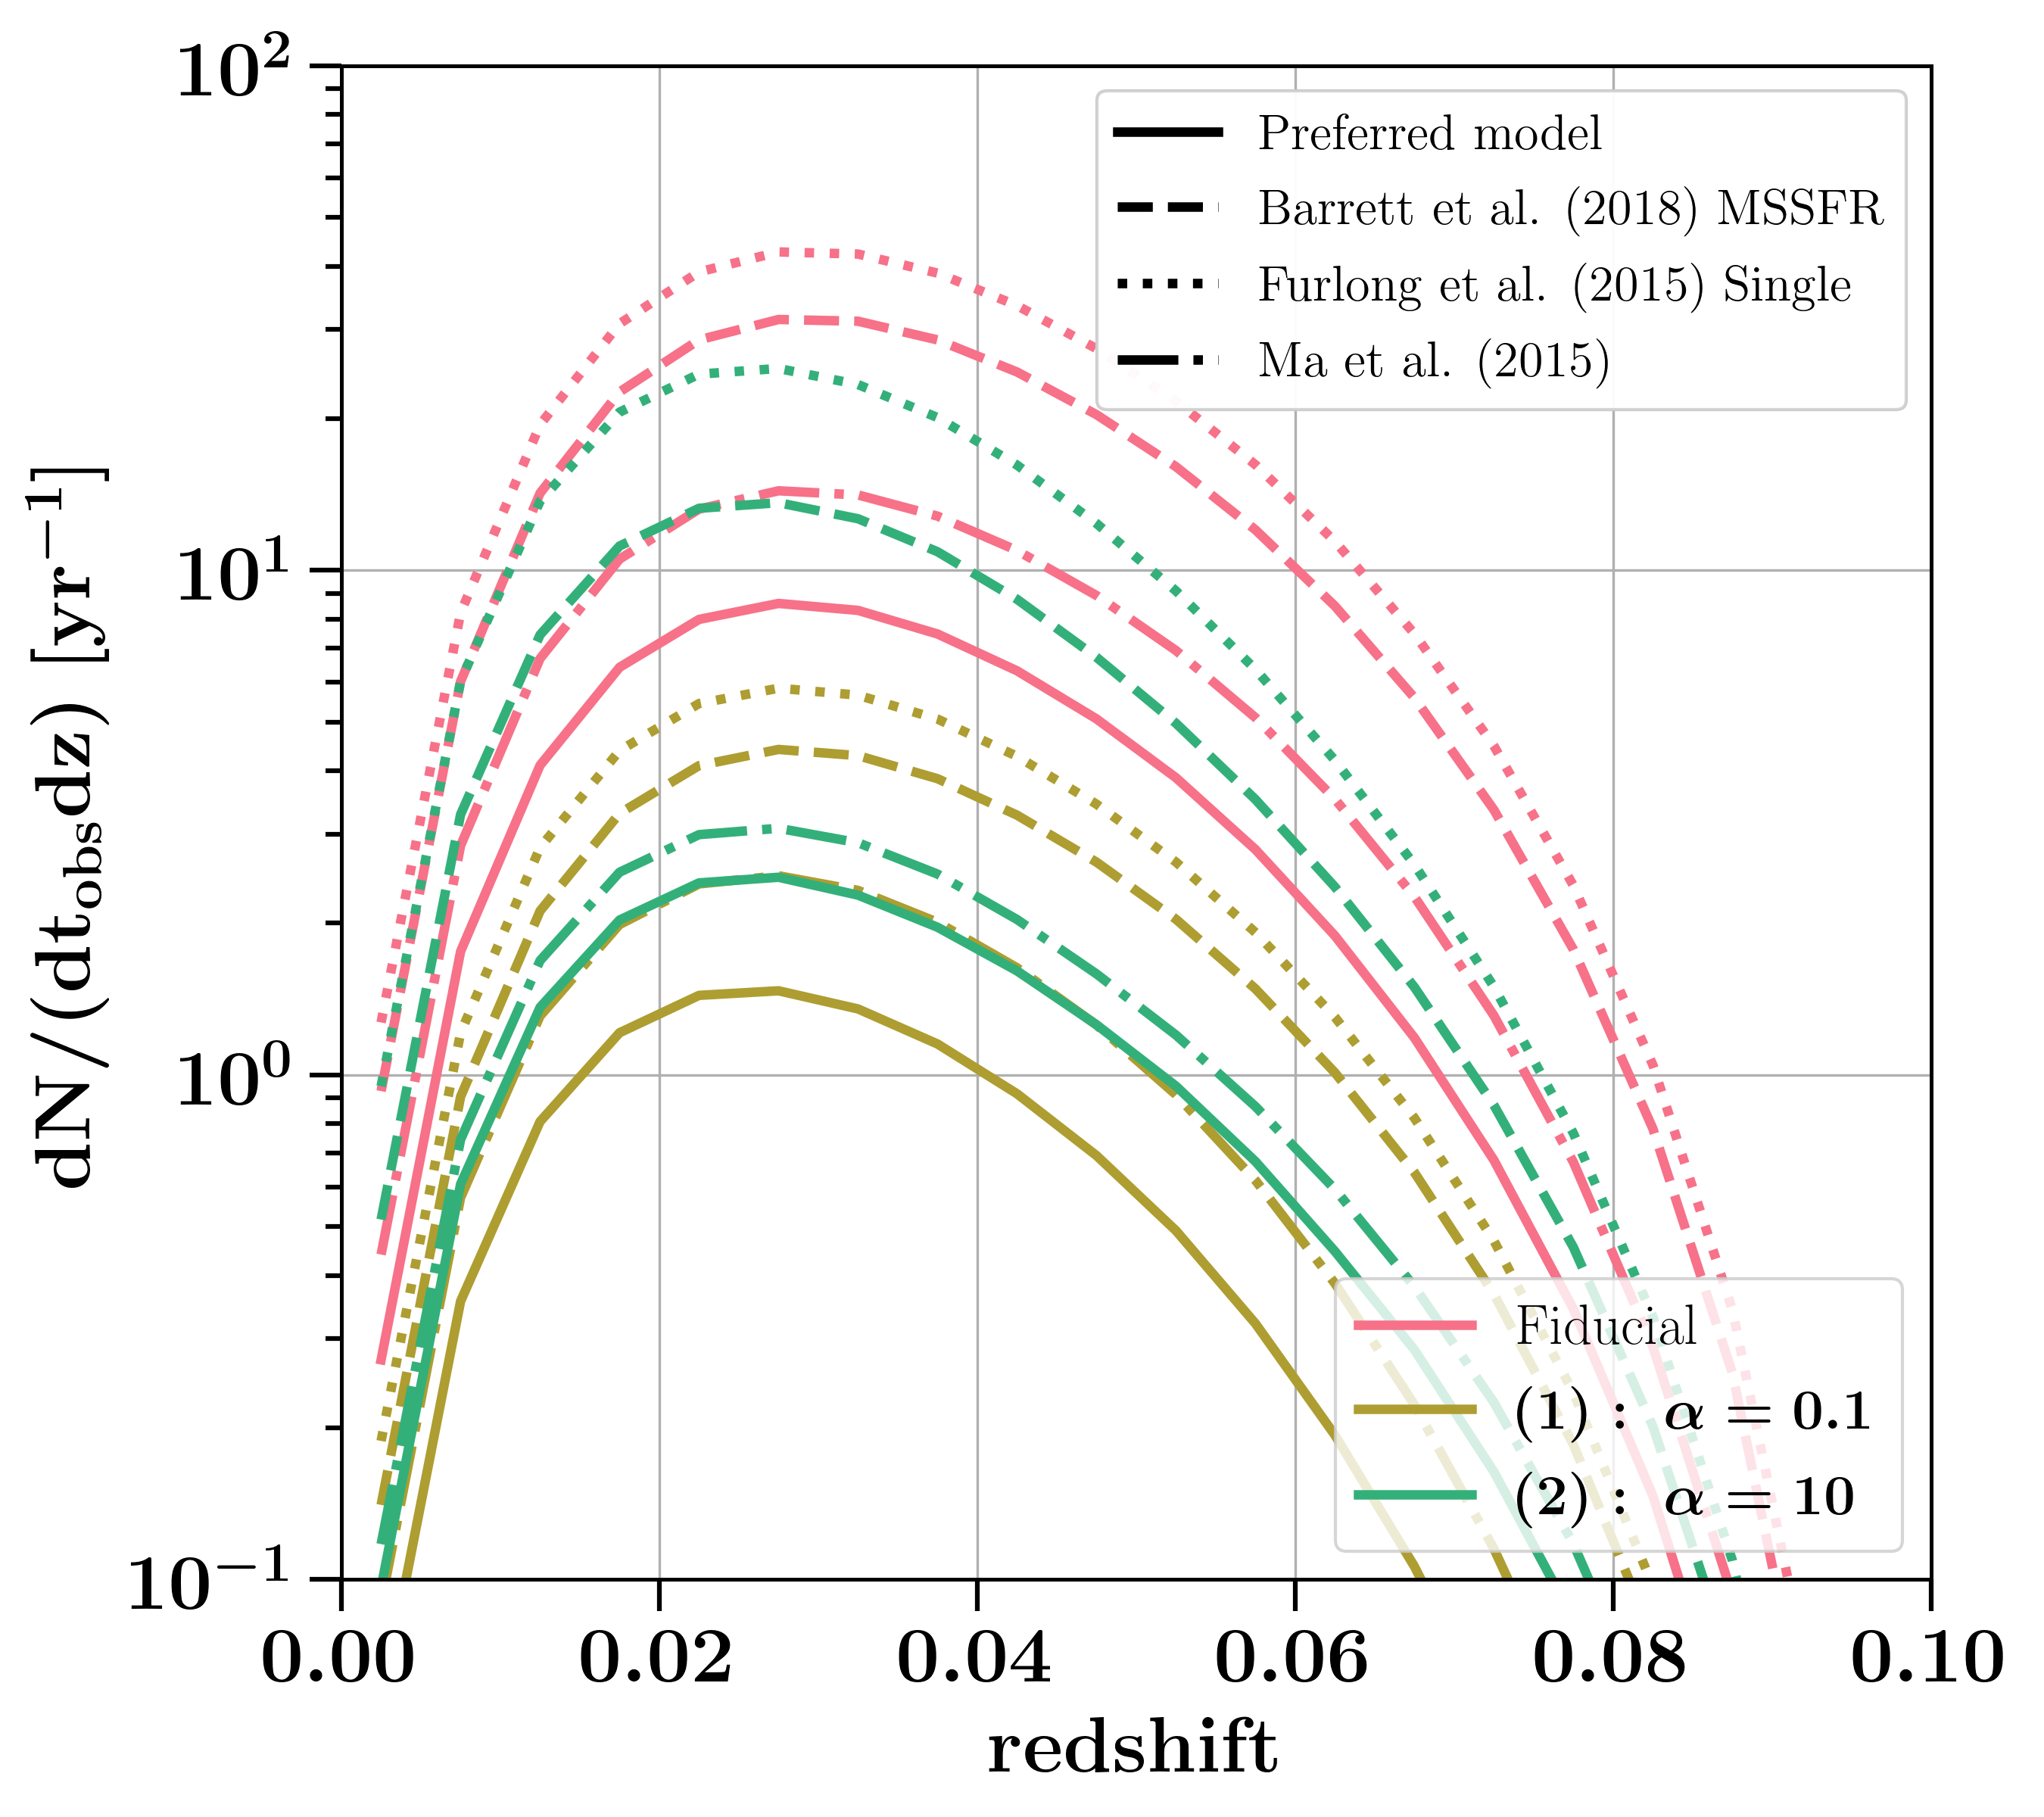
\includegraphics[width=1\columnwidth]{../PlottingScripts/4_MSSFR_observed/TotalMergerRateRedshiftObs-BHNS_models.png}
%   \caption{redshifts at which we will see \bhnsSingle mergers with LVK \ac{GW} network
%   }
%  \label{fig:BHNS_DCO_LVK-redshift}
%\end{figure}
%%


%\section{Other implications}
%
%
%\begin{itemize}
%	\item BH--Pulsar systems
%	\item LISA
%	\item UFD galaxies
%	\item 
%	\item Variations
%	\item 
%\end{itemize}

%%%%%% UFD: 

%% FROM MIKE ZEVIN

%ally (Qian &Woosley 1996; Thompson et al. 2001; Roberts et al. 2012; Martínez-Pinedo et al. 2012) and observation- ally (Wallner et al. 2015; Hotokezaka et al. 2015) as a pro- duction site for heavy r-process elements. The neutron-rich ejecta from neutron-star mergers (NSMs) is theorized to fill these open gaps in the periodic table, polluting the Uni- verse with the heaviest naturally-occurring elements (Lat- timer & Schramm 1974, 1976; Eichler et al. 1989; Meyer 1989; Davies et al. 1994; Ruffert et al. 1997; Rosswog & Liebend 1999; Freiburghaus et al. 1999). Over

%A number of observational campaigns have investigated
%the ubiquity of r-process enhancement in GCs. From a sam- ple of 11 low-metallicity GCs, Roederer (2011) found that 4 GCs showed clear signs of large r-process dispersion, 5 GCs showed no dispersion, and 2 GCs were more ambigu- ous with smaller levels of dispersion. Out of the 5 GCs that had no clear r-process dispersion, 2 show bimodal chemi- cal abundance ratios, possibly suggesting formation through the merger of 2 separate GCs that may have washed out ini- tial star-to-star dispersion (Yong & Grundahl 2008; Marino et al. 2009; Carretta et al. 2010).

\section{Discussion }
\label{sec:discussion}
%%%
%
%




Extremely cool MZ paper: 
\url{https://arxiv.org/pdf/1910.00597.pdf}
The Mass-Metallicity and the Fundamental Metallicity Relation revisited on a fully Te-based abundance scale for galaxies [GA] The relationships between stellar mass, gas-phase metallicity and star formation rate (i.e. the Mass-Metallicity, MZR, and the Fundamental Metallcity Relation, FMR) in the local Universe are revisited by fully anchoring the metallicity determination for SDSS galaxies on the Te abundance scale defined exploiting the strong-line metallicity calibrations presented in Curti et al. (2017)




The third observing run (O3) just finished and five alerts are already announced for \ac{GW} event candidates classified as a \bhnsSingle merger \citep[see the GCN alerts  by][]{GCNS190814bv,GCNS190910d,GCNS190923y, GCNS190930t,GCNS191205ah}.  

\subsection{Delayed versus Rapid}
\label{subsec:discussion-delayed-vs-rapid-SN-remnant-mass}

The {rapid} prescription assumes \ac{SN}  explosions occur within 250 ms (compared to longer timescales assumed for the delayed prescription) and reproduces, by construction,  the  lower remnant mass gap between NSs and BHs that is apparent from  X-ray binary observations 
\citep{1998ApJ...499..367B, 2010ApJ...725.1918O, 2011APS..APRH11002F} by a lack of BHs in the mass range between about the heaviest neutron stars  $\sim$ 2--3\Msun \citep{2016ARA&A..54..401O, 2017ApJ...850L..19M, 2019NatAs.tmp..439C,2019arXiv190801012T,2020arXiv200106102S} and  BHs of $\sim$ 4--7\Msun. \question{Should I discuss that  merging \ac{NS} product can fall in \ac{BH} gap?} % \citep{2015ApJ...801...90P,2019ApJ...882L..24A}. 
% 
	It is still under debate whether this lower \ac{BH} mass gap exists. Theoretical models of supernovae both predict a gap \citep{2014ApJ...785...28K,2015ApJ...801...90P} and no  gap (e.g. \citealt{1995ApJS..101..181W,2001ApJ...554..548F,2019arXiv191001641E, 2020arXiv200304320C})  in the mass distribution between \ac{NS} and \ac{BH} remnant masses. But see also \citet{2020MNRAS.491.2715B} who point out that it is very challenging to model remnant masses from supernovae explosions and that the compactness measure that is often used in these \ac{SN}  remnant mass studies is not a good metric for explodability of the supernova. 
	Moreover, \citet{2012ApJ...757...36K}   show evidence that the apparent observed mass gap from BHs in X-ray binaries could be caused by systematic offsets in the \ac{BH} mass measurements.  
	More recently, \citet{2019Sci...366..637T} found evidence for a $3.3_{-0.7}^{+2.8}$\Msun mass \ac{BH} observed in a non-interacting binary with a red giant, which is in addition of earlier observation of a speculated $\sim 2.44\pm0.27$\Msun \ac{BH} \citep{2002A&A...392..909C,2010AAS...21541905R,2011arXiv1107.1537D}. 
	In addition,  \citet{2016MNRAS.458.3012W,2019arXiv190407789W} studied microlensing events of BHs based on  observations from OGLE-III and Gaia data release 2.  
	They find evidence for a continuous distribution of stellar remnant masses and disfavor a mass gap between NSs and BHs (unless BHs receive natal-kicks above 20-80\kms).   
	In addition, the LIGO-Virgo Collaboration reported at the time of writing three candidate \ac{GW} events in their O3 observation run with at least one component in the lower mass gap \citep{GCNS190924h,GCNS190930s,GCNSS200115j}.	
%	We therefore conclude that based on the above, there is no clear evidence that the rapid remnant mass prescription  should be preferred in population synthesis simulations. 
	
Moreover, \citet{2018MNRAS.481.4009V} show that the delayed prescription better matches the observed distribution of masses of Galactic double \ac{NS} systems. 
We  therefore adopt the delayed remnant mass prescription and vary this to the rapid prescriptions as one of our model variations (see Table~\ref{tab:variations-BPS}). \\
	


\subsection{ECSN prescription}

More recently, \citet{2004ApJ...612.1044P} argued  that helium core ranges of 1.4--2.5\Msun are more realistic and \citet{2015ApJ...801...32A} and Vinciguerra. (in prep.) show a different electron-capture range (resp. 2--2.5\Msun and 1.85--2.25\Msun, where the latter is based on \citealt{2008ApJS..174..223B}) could better reproduce observations of neutron stars. \floor{This might influence the rate a lot - re-discuss in discussions?}. 



\href{https://arxiv.org/abs/2001.06025}{SFR-mass relation paper note} \citep{2020arXiv200106025K}
\subsection{initial conditions uncertainties}
from de Mink and belczynski 2015: There are relatively few formation channels for double compact object mergers. For a given model of evolution, these formation channels originate from a rather narrow volume of initial parameter space (the formation volume). Change of initial conditions alters the number of the progenitor binaries in the formation volume, but has very little effect on the binary merger properties. This insensitivity is not just connected to the specific initial conditions considered here, but is of more fundamental nature. It is a robust result that has also been found in connection to other compact object binaries. For example by Kalogera $\&$ Webbink (1998) in the context of low-mass X-ray binaries, and see also Belczynski et al. (2002).

IMF slope might be more shallow \citep{2018Sci...359...69S}

\subsection{other}


\url{https://arxiv.org/abs/1910.04168} discusses that the SF and galaxy mass is not well known for redshifts higher than 2. and helps improving this. 


We discuss prospects of identifying and characterizing black hole (BH) companions to normal stars on tight but detached orbits, using photometric data from the Transiting Exoplanet Survey (\url{https://arxiv.org/abs/1808.10856#})

\url{https://arxiv.org/abs/1910.00822}
We study the prospects of searching for black hole (BH) binary systems with a stellar-mass \ac{BH} and a non-compact visible companion, by utilizing the spectroscopic data of Large Sky Area Multi-Object Fiber Spectroscopic Telescope (LAMOST). they predict how many can be found. 


BHNS CAN HELP FIND DETECT THE EOS  \url{https://arxiv.org/pdf/1103.3526.pdf}
%Using recent post-Newtonian expressions and realistic equations of state to model these scenarios, we find that point-particle templates are sufficient for the detection of black hole-neutron star inspiralling binaries, with a loss of signals below 1% for both second and third-generation detectors. Such detections may be able to constrain particularly stiff equations of state, but will be unable to reveal the presence of a neutron star with a soft equation of state.


\subsection{BH--Pulsars}

Detecting  \bhnsSingle systems with a pulsar provide a unique laboratory to test general relativity and alternative theories of gravity \citep{Wex:1998wt,KRAMER2004993} and will enable high precision  measurements of the  properties of black holes    \citep{1975ApJ...198L..27B,1975SvAL....1....2B}.  \floor{this last part is about BHNS with pulsar specifically. Move this to BH--Pulsar discussion?}
%
%
From \href{https://arxiv.org/abs/2003.02277}{Mapelli group}: 
%The lack of observations of BH-pulsar binaries with current radio facilities is not surprising: Pfahl et al. (2005) estimate that there are no more than one \ac{BH} - recycled pulsar binary in the Milky Way for every 100 - 1000 BNSs, of which 15 are currently known (Tauris et al. 2017; Farrow et al. 2019).
%


%\https://arxiv.org/abs/1804.06014
%We have performed population synthesis calculation on the formation of binaries containing a black hole (BH) and a neutron star (NS) in the Galactic disk. Some of important input parameters, especially for the treatment of common envelope evolution, are updated in the calculation. We have discussed the uncertainties from the star formation rate of the Galaxy and the velocity distribution of \ac{NS} kicks on the birthrate (∼0.6−13Myr−1) of BH/NS binaries. From incident BH/NS binaries, by modelling the orbital evolution duo to \ac{GW} radiation and the \ac{NS} evolution as radio pulsars, we obtain the distributions of the observable parameters such as the orbital period, eccentricity and pulse period of the BH/pulsar binaries. We estimate that there may be ∼3−80 BH/pulsar binaries in the Galactic disk and around 10\% of them could be detected by the Five-hundred-meter Aperture Spherical radio Telescope.

\subsection{Variations}
\label{subsec:bhns-discussion-variations}

\href{https://arxiv.org/pdf/1708.07885.pdf}{compare with variations this paper}


\subsection{learn about \ac{BH} mass function}
%
see \href{https://arxiv.org/pdf/2002.02981.pdf}{this paper}

\subsection{Rates ratios}
From Dominik2012
One exception is the Optimistic \ac{CE} model, in which the merger rate per unit volume is large enough (while still being lower than for NSNS systems at all redshifts) that BH--NS detection rates are larger than NSNS rates because they are observed farther (see Table 1 and Figure 6).

%
\subsection{relativeRates}
%


\subsection{BH--NS}
might be needed for early r-process enrichment \href{https://arxiv.org/pdf/1601.06966.pdf} t%202020-02-06%2022.23.12.png?dl=0

% UNDO DO THIS FOR UFD galaxy rates plots
%
%\begin{figure*}
%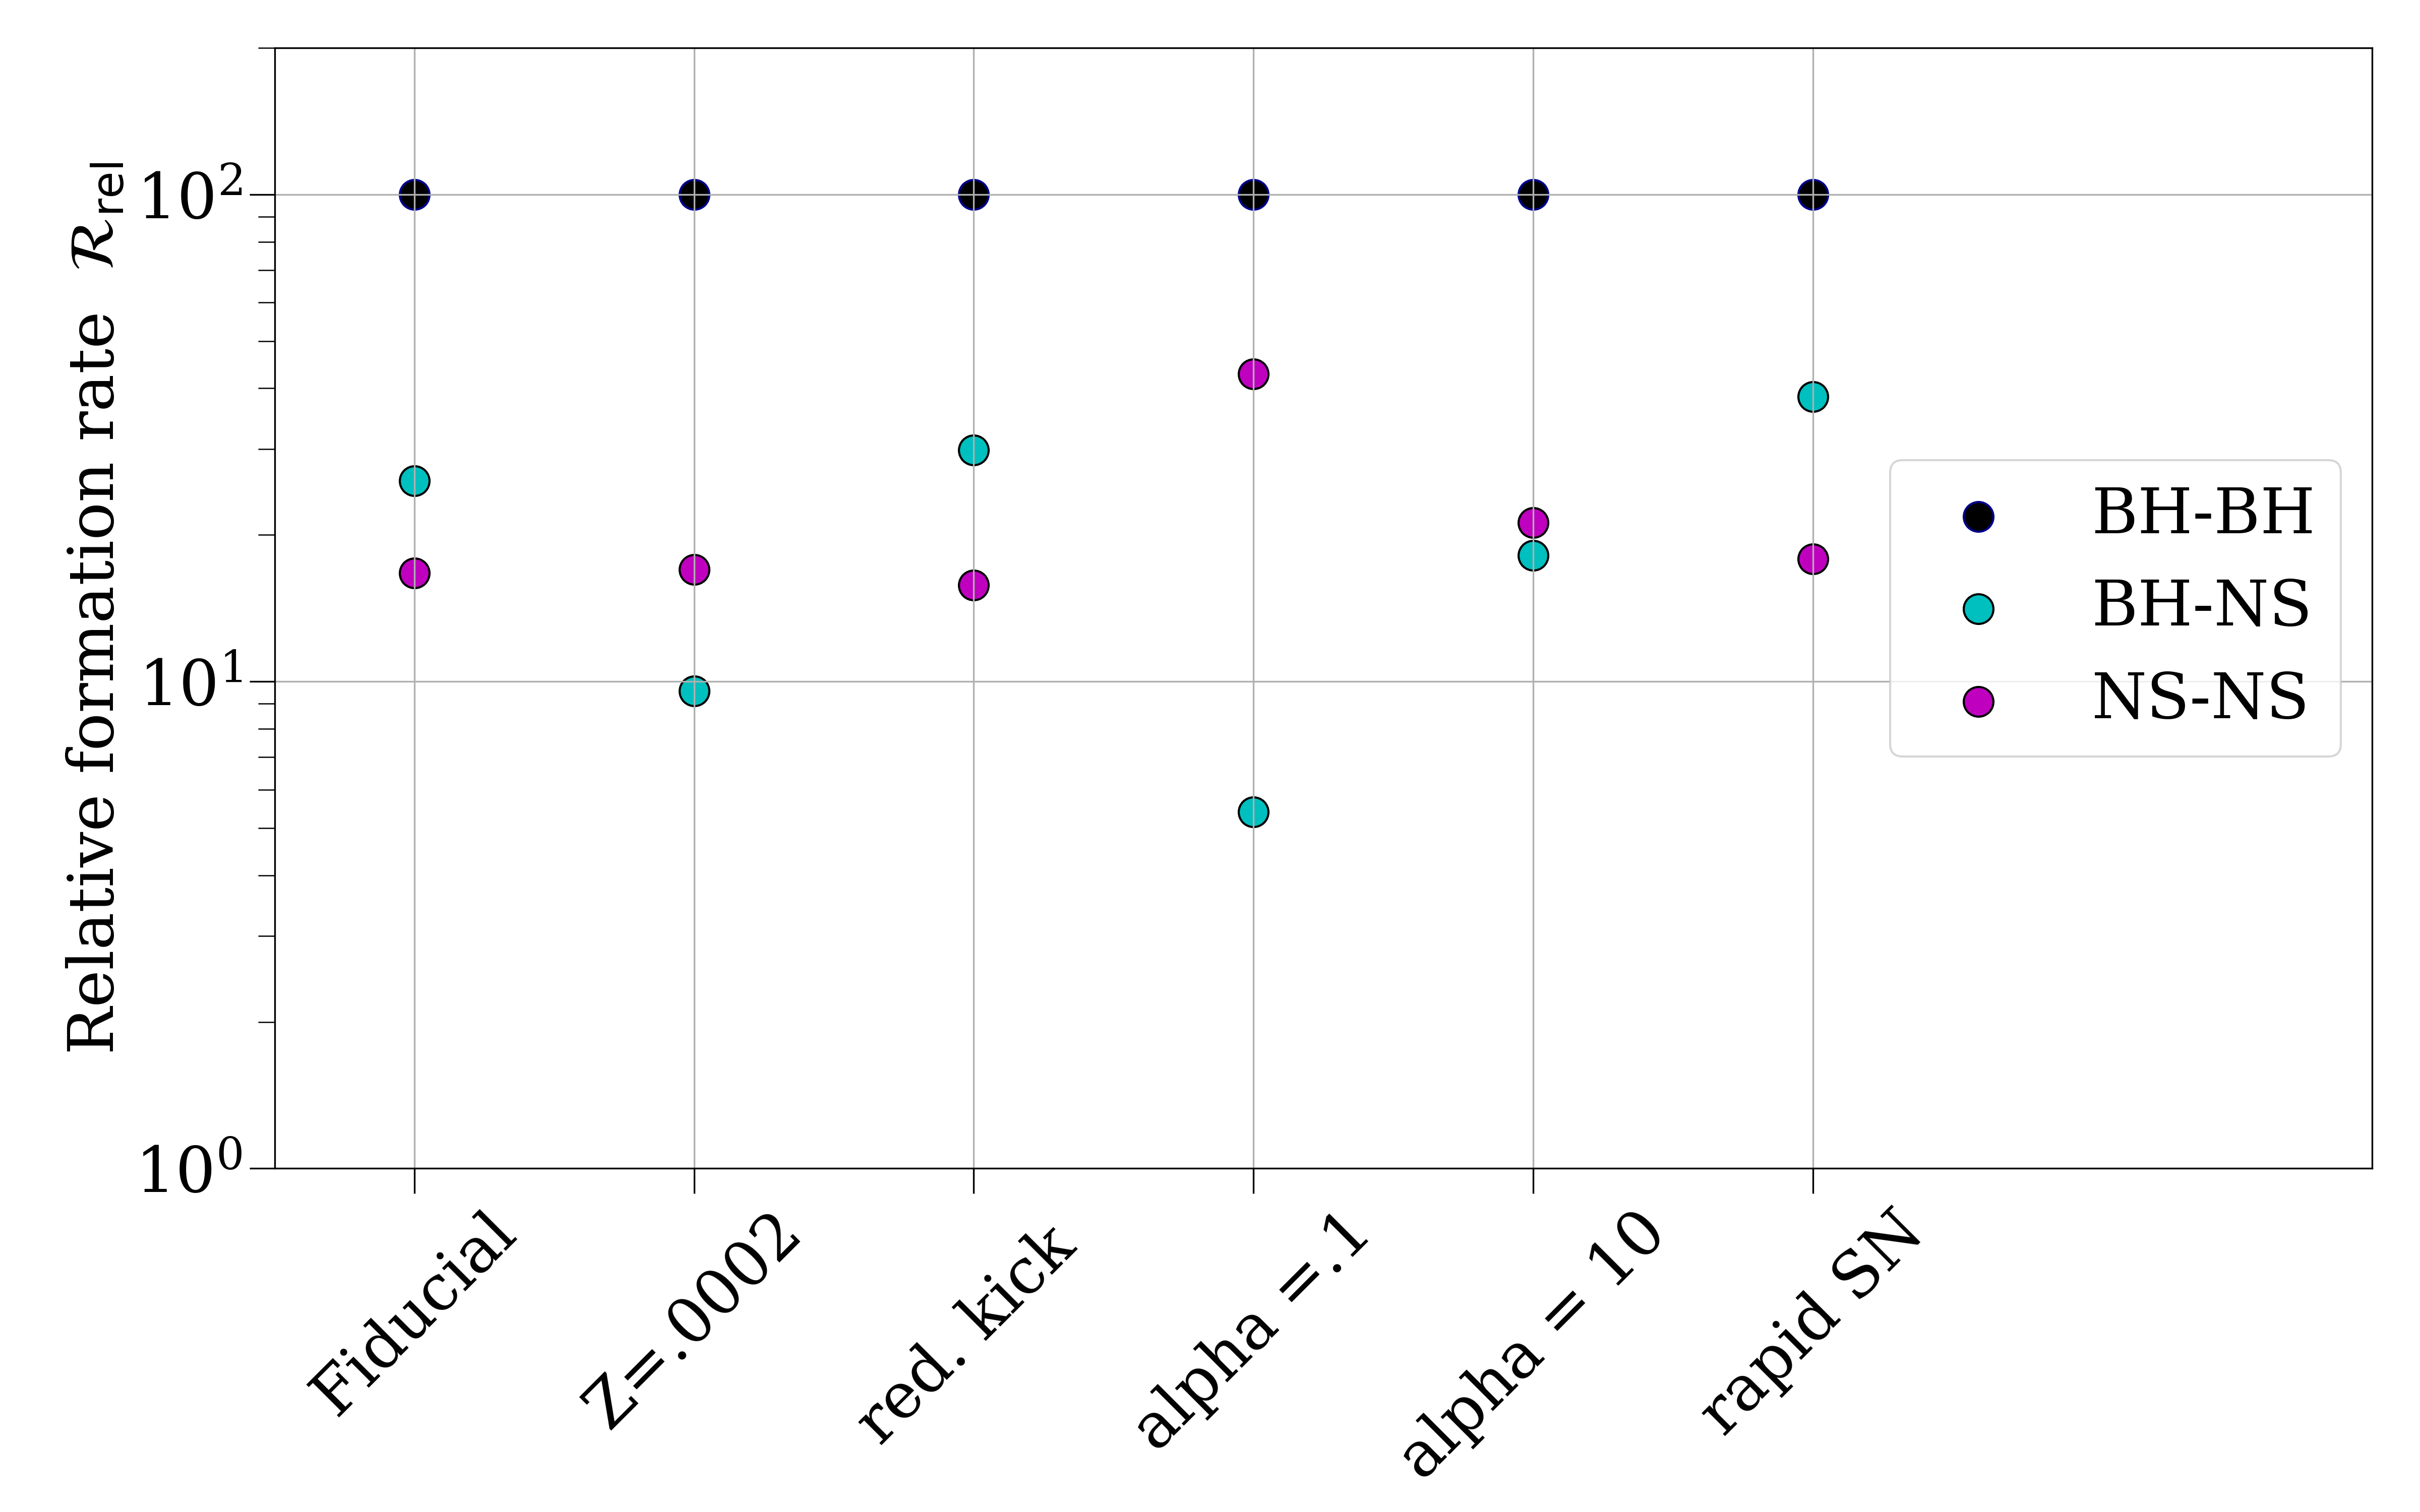
\includegraphics[width=.8\textwidth]{../PlottingScripts/imagesUFDandRatios/relativerates_formation.png}
%   \caption{ }
%  \label{fig:BHNS_DCO_j}
%\end{figure*}
%%
%
%%
%\begin{figure*}
%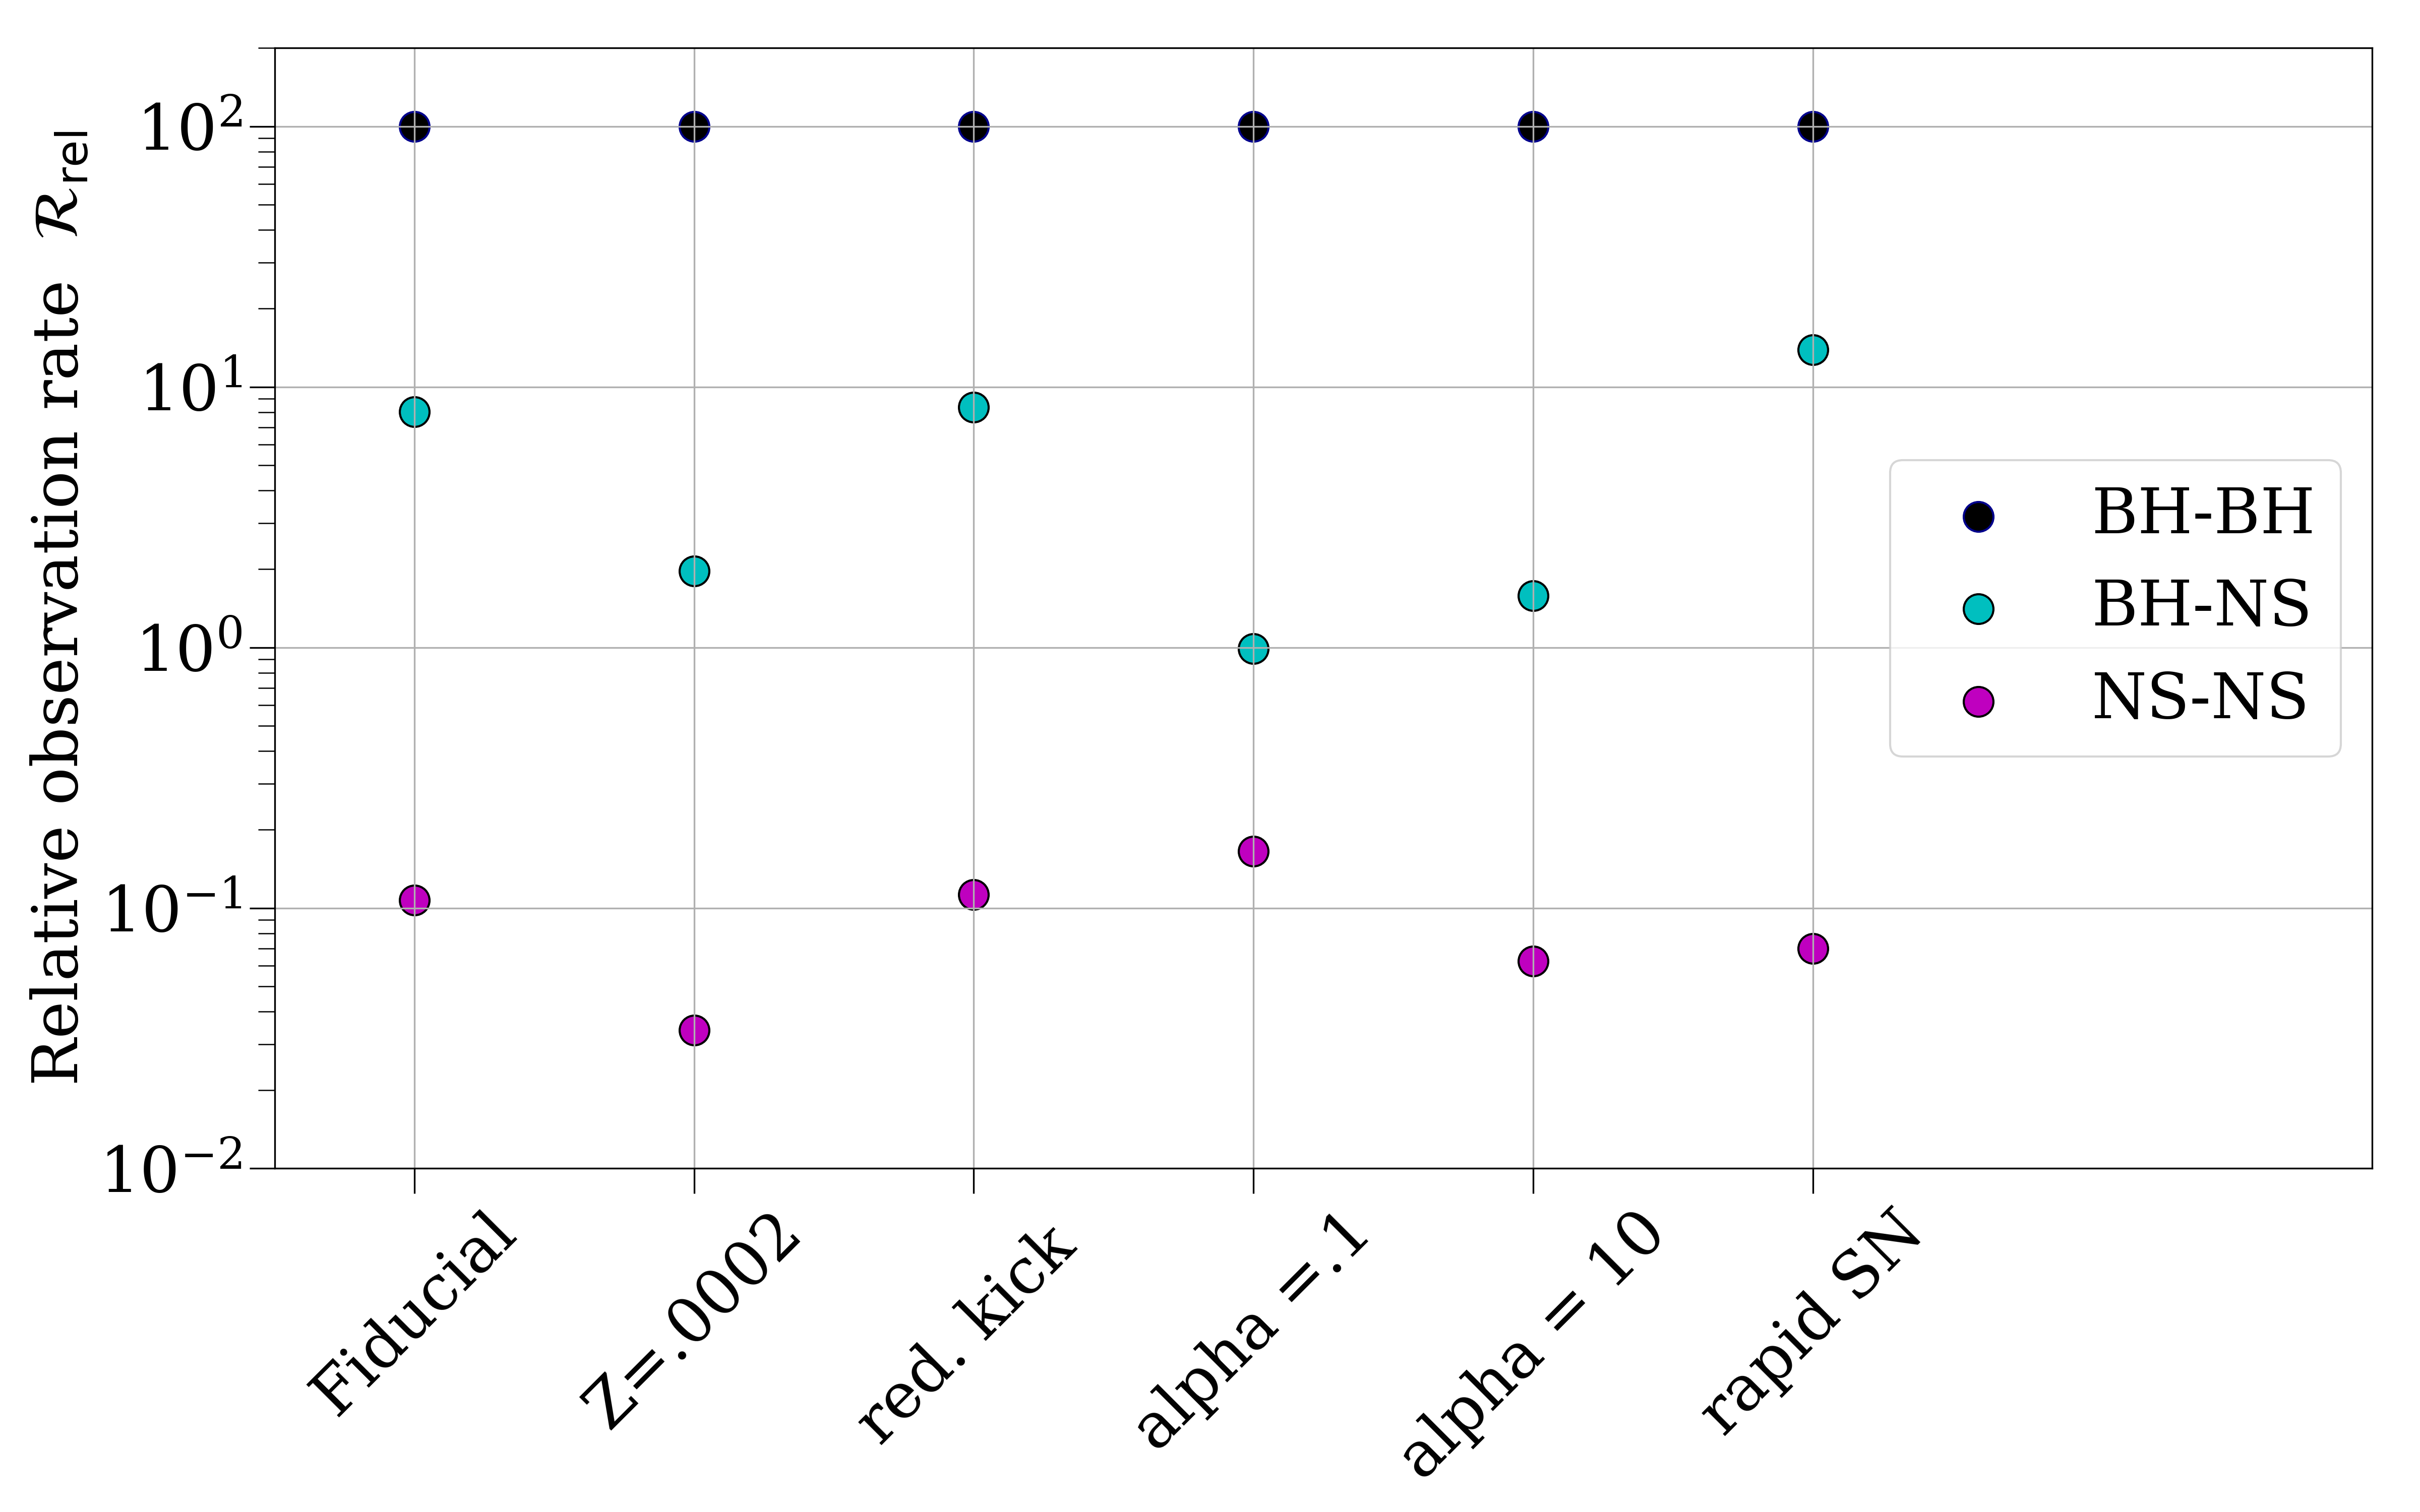
\includegraphics[width=.8\textwidth]{../PlottingScripts/imagesUFDandRatios/relativerates_observed.png}
%   \caption{ }
%  \label{fig:BHNS_DCO_k}
%\end{figure*}
%%



\subsection{Parameter study}


%\subsection{Galactic BH--NS }
%
%
%
%
%\subsection{BH--MSP systems}
%
%
%\subsection{standard candals}
%The observed drop-off in the abundance of  45Msun black holes can be used to probe cosmic expansion by making binary black hole mergers``standardizable`` (Farr et al. 2019). 
%
%
%\subsection{Arxiv discussion}
%% The precise determinations of stellar mass at $\sim$1% provide important constraints on stellar evolution models. Accurate parallax measurements can also serve as independent benchmarks for the next Gaia data release. Aims. We aim at measuring the masses and distance of binary systems with a precision level better than 1% using a fully geometrical and empirical method. http://arxiv.org/abs/1910.03393
%
%
%
%
%
%
%\section{stuff from papers:}
%
%%\subsection{Simulation set up}
%%\begin{itemize}
%%	\item one model
%%	\item 30 different metallicities
%%	\item 1 million binaries per metalicity
%%	\item pop synth + \ac{MSSFR} 
%%	\item how do we select BH--NS and NS--BH
%%\end{itemize}
%%
%%
%
%\subsection{IMF}
%From \url{https://arxiv.org/pdf/1910.01126.pdf}
%
%The present--day generally accepted IMF[11] can thus be well represented by the canonical two-part power-law function with$ x = 0.3$ for $0.1 < $m/Msun $< 0.5$ and $x = 1.3 $for $0.5 leq$ m/Msun $< 150$. This IMF shape was confirmed[12]
%
%Recent observations have uncovered a dependency of the IMF on metallicity and density[15], [16], and infrared surveys have shown stars to form in long and thin molecular cloud filaments[17], challenging the gravo-turbulent theory of the IMF.

%
%\subsection{wind prescription}
%we use wind mass loss rates by \citet{2000A&A...362..295V,2001A&A...369..574V}. Where the line-driven wind loss scales with metallicity as $Z^{m}$ with $m\approx 0.69$, which is found to be  in agreement with  observations \citep[][]{2007A&A...473..603M}. Although the amount of mass loss is uncertain \cite{2014ARA&A..52..487S, 2017A&A...603A.118R} -  see also a review by \citep{2014ARA&A..52..487S} for more information.
%\subsection{case BB MT}
%The starting point of all these calculations (tight systems containing a naked helium star and a \ac{NS} with orbital period, Porb $< 2$ days) is a continuation of the expected outcome of common envelope (CE) evolution in high-mass X-ray binaries. Of particular interest is mass transfer by Roche-lobe overflow (RLO) initiated by the helium star expansion after core helium exhaustion (so-called Case BB RLO).
%%Tauris 2015
%\subsection{USSN}
%we now don't allow USSN for case BB onto a \ac{BH} 
%
%\textbf{tauris2015}
%I found this in Tauris2015, when they calculate the USSN rate : 
%"On the other hand, we have to include similar systems producing black hole–NS binaries and also add the number of systems (a factor of a few) which were disrupted as a consequence of the dynamical effects of the second  \ac{SN} explosion, and are therefore not contributing to the estimated merger rates quoted above."
%Which seems to suggest that Tauris thinks that USSN are formed in BH-NS binaries, if the \ac{BH} forms first (and thus the USSN star is the pre-NS)  %
%%https://iopscience.iop.org/article/10.1088/2041-8205/778/2/L23/pdf
%The explosion of ultra-stripped stars in close binaries can lead to ejecta masses $\leq0.1 M_{\odot}$ and may explain some of the recent discoveries of weak and fast optical transients.
%
%
%The total amount of helium in this envelope is 0.033Msun. The ultra-stripped nature of our model is achieved because the helium star is forced to lose (almost) its entire envelope in a very tight orbit where a \ac{NS} can fit in.
%%https://watermark.silverchair.com/stv990.pdf?token=AQECAHi208BE49Ooan9kkhW_Ercy7Dm3ZL_9Cf3qfKAc485ysgAAAl4wggJaBgkqhkiG9w0BBwagggJLMIICRwIBADCCAkAGCSqGSIb3DQEHATAeBglghkgBZQMEAS4wEQQMDnT5Wc8OYSqJBrW0AgEQgIICERaGRzgIOiqhB_3Emkt0HOzs_QrLS9snb99E0wHmM41oca9I5z4tNYkEpiPlg7Z8xDdOD31N7qwvGiSUOH5vGJxEKPEK5WHAe8-6NIYc70InoJ_ApOZUU_jW8SQu0ukAUlOaCyzyUGWPJkVTHgEb5SSRHq03kw-6TIQHVarRQo5EzejN1fXlOZgAJ6claZL7gPji9M6WwEZm4e_6Cxzczm9ekynhHy05_H7mC9sVcejPbp-33_yzxCpL6kkOwEvXwbOV4_WC6F_Effjet5FWIj3oh948r37v1NHVuk2K6GGO7A10h9eExvTZzXDL06G2qzRqj2WOKmWKgB1iloWJdhECyoIrjVYPV8gKgsw9SvztCxX7VULHAw42BG4derqsGNmT-bFc1LIbDygwQ8rS3Uuxd-0DDf71J-d5dsxfpf78xl1mpU-uxJaGqbm--h0pAQpOnX_Y2i9k1pIriaxyi4KwVRptO-WqrKYSxySBMZOGHz_SqBoCWjMYruBoVVaK5iTye1X3vZiN-XzjDRGdAZti1IlogcghQzpf9WB0vfRUhWvWqfRMQ0dtlX2t0r9l8-YOVtpAF7SoKLIKioJzWNIM1mONUpVVdWD5z4QJhfe7n72Vlx3yxBZ-J4eFpOxhFfn4rIj4H63Nb2C0CCNcCqYfMpqsZXu_3iLlatfVL2-6DrA1Z3kPAqn4Cq3tFNFbKag
%
%
%In other words, ultra-stripped SNe are exploding stars which contain envelope masses $\leq 0.2$M and having a compact star companion. The compact nature of their companion allows for extreme stripping in a tight binary, in some cases yielding an envelope mass $\leq 0.008$Msun %10.1093/mnras/stv990
%%Ultra-stripped supernovae: progenitors and fate 
%
%It has recently been demonstrated (Tauris et al. 2013, 2015)
%that close--orbit DNS systems (i.e., those that are tight enough to merge within a Hubble time due to GWs) must form via ultra-stripped SNe when the last star explodes. The reason being that Case BB RLO, i.e., mass transfer via Roche-lobe overflow from a naked helium star in the post-HMXB/post-CE system, causes the \ac{NS} to significantly strip its evolved helium star companion almost to a naked metal core prior to its explosion. This has an important effect on the number and properties of surviving DNS systems-in particular, in terms of their kinematic properties-as we shall discuss rigorously in more
%%Tauris DNS 
%
%
%% from Combine 
%If the exploding star forms the second-born compact star of the binary, it undergoes an ultra-stripped  \ac{SN} (Tauris et al. 2013, 2015; Suwa et al. 2015; Moriya et al. 2017) because of severe mass stripping by the nearby compact object, leaving an almost naked metal core at the time of the explosion. For such ultra-stripped SNe we apply w1Drms $= 30$ km /s,
%in accordance with the many double \ac{NS} systems observed with small eccentricities of $e <
%\sim 0.2$ (Tauris et al. 2017).\\
%
%
%\textbf{COSMIC has it:}
%\url{https://cosmic-popsynth.github.io/docs/latest/inifile/index.html}
%Reduces kicks according to the sigma div selection for ultra-stripped supernovae which happen whenever a He-star undergoes a \ac{CE} with a compact companion
% 
%
%\subsection{Optimistic vs Pessimistic}
%\textbf{Vigna--Gomez 2018}
%We allow donor stars which engage into a \ac{CE} phase during hydrogen shell burning (HG) to survive the event and expel the common envelope if allowed by the energy condition. This assumption is labeled ``optimistic``CE in the literature (Dominik et al. 2012), while the alternative, ``pessimistic`` CE, always leads to a merger for HG donors.
%
%\textbf{Dominik2012:}
%The impact of the \ac{CE} outcome on binary populations
%depends strongly on the evolutionary stage of the donor, as first discussed in Belczynski et al. (2007). The Standard model does not allow for \ac{CE} events with HG donors. These stars are not
%expected to possess a clear core-envelope structure (Ivanova and Taam 2004), thus making it difficult for them to eject their outer layers during the \ac{CE} phase. In our Standard model all \ac{CE} events with HG donors lead to a prompt merger before a DCO binary is formed, regardless of the aforementioned energy balance. The
%%http://dx.doi.org/10.1088/0004-637X/806/2/263
%
%
%\textbf{Mapelli}
%Finally, we have revised the treatment of Hertzsprung gap (HG) donors in CE: HG donors are assumed to always merge with their companions if they enter a \ac{CE} phase. This is justified by the fact that HG stars have not yet developed a steep density gradient between core and envelope, and allows us to match the merger rate of BHBs (Mapelli et al. 2017) inferred from LIGO--Virgo observations (Abbott et al. 2016a).
%%arXiv:1806.00001v1
%
%\textbf{Wiktorowics and Belczynksi}
%%https://arxiv.org/pdf/1907.11431.pdf
%We assume that non-DCO mergers occur in the follow- ing situations:
%(1) failed envelope ejection during a \ac{CE} event (e.g. Justham et al. 2014),
%(2) donor in a \ac{CE} phase haven’t developed a clear boundary between core and the envelope (e.g. MS and HG donors; Ivanova and Taam 2004),\\
%
%\textbf{Olejak Belczynski }
%2.3. Hertzsprung gap stars in common envelope
%We calculated two \ac{CE} models (marked as A and B) which represent different scenarios for binary system with Hertzsprung gap star (HG) as a donor in the \ac{CE} phase. In model B we assume that all of such binary systems merge during \ac{CE} and possibly create a single BH. In model A we let such a system to survive \ac{CE} phase on the energy balance calculations (Webbink 1984). Currently it is not well known which scenario operates (Ivanova and Taam (2004)).
%
%%We present population synthesis statistical estimates of the cur- rent Milky Way black hole population properties. We used the most current version of the StarTrack code with standard physics (Sec. 2) and processed the data with the new star formation rates and metallicity distribution model of our Galaxy, based on theo- retical models and observations. We show results for two mod- els: A and B, which correspond to different scenarios of a \ac{CE} phase (Sec. 2.3). We find that:
%%1) At the current moment the Milky Way (disk+bulge+halo) contains about 1.6 × 108 single black holes with average mass 13 M⊙ and 9.3 × 106 black holes in binary systems with average mass 19 M⊙.
%%2) There are three main formation channels of single BHs: ∼ 35% are remnants of massive single star evolution, ∼ 40% formed in binary systems merger, ∼ 25% of single BHs orig- inate from disrupted binary systems during black hole/neutron star formation.
%%3) The most massive black hole in simulation comes from old, low in metal environment of Galactic halo. It formed in MS-He stars coalescence and its mass is as large as ∼ 130 M⊙.
%%4) Black holes in binary systems constitute ∼ 10 % of the whole Galactic \ac{BH} population. Most of BHs in binary systems are in BHBH configuration. The fraction of black hole binaries with non compact companion is small, about 0.3 % of all Galactic BHs.
%%-We estimate how double compact object systems merger rates (BHBH, BH-NS and NSNS) have changed along with the Galaxy star formation. Current Galactic merger rates depend on model and they are estimated at ∼ 81/3 Myr−1 for BHBH, ∼ 9/1 Myr−1 for BH-NS and ∼ 59/14 Myr−1 for NSNS systems.
%%5) We constrain that only ∼ 0.005 % of total Galactic halo mass (including dark matter) could be hidden in the form of stellar ori- gin BHs which are not detectable by current observational sur- veys
%%6) Only ∼ 5 % of single BHs and 0.001 % of binary BHs have enough high velocities to escape from Galactic potential.
%%On Figure 6 we show how the total number of BHs formed in the Milky Way have been changing since the Milky Way forma- tion till current time with assumed star formation rates and star metallicity distribution (Sec.2.5) for two evolutionary models A and B.
%\subsection{DELAYED FRYER}
%1) The defaults are in some sense meaningless. They are intended as something like a best guess, but we will always want to demonstrate how variations away from this default affect our conclusions. For this reason I don't think it really matters which one we choose as default.
%2) Rapid reproduces NS-BH mass gap. By construction, it does this. However since it is not clear whether this gap is real, or due to some selection effect, I do not find this a compelling reason to prefer it 
%3) The rapid prescription does not reproduce the observed DNS masses. As we showed in Alejandro's paper, the rapid prescription (combined with other COMPAS defaults) does a miserable job of reproducing the observed DNS masses. Delayed did a bit better.
%4) For massive BHs formed through complete fallback, the two prescriptions are the same, so again there is no real reason to prefer one over the other
%From Alejandros paper:
%In fact, the  RAPID  \ac{SN} mechanism (01) allows for low-mass NSs which would be difficult to differentiate from NS–white dwarf binaries; there are several non-confirmed DNSs or poorly constrained DNS masses in the region favoured by the “rapid” mechanism (01) (Ozel et al. 2010; Ozel $\&$ Freire 2016). On the other hand, the seven existing well-constrained mass measurements in this study are inconsistent with the predictions of the fiducial model (01) at a $>$ 4sigma level. None of these seven measurements fall below a chirp mass of 1.1 Msun, while 83 per cent of DNSs in the fiducial model have lower chirp masses. This suggests that the RAPID mechanism under-predicts the amount of collapsed mass for the lowest-mass NSs for both ECSNe and USSNe.
%
%Fryer rapid, on the other hand, is hardcoded to have a maximum of 2.0 solar masses. So, if you use the rapid Fryer, it will make no different.\\
%
%
%\textbf{ERTL and Woosley 2019}
%ERTL and Woosley \url{1910.01641} find : Lower mass black holes exist though, on down to the maximum neutron star mass. There is no unpopulated ``gap``.
%
% The most obvious difference of the helium-star explosions compared to the single-star models of Sukhbold et al. (2016) (see also Appendix A) is the greater number of cases with significant fallback.
% 
% These fill in a ``gap`` in the remnant mass distribution that might have existed between gravitational masses of about 2 to 6Msun. Most cases where black holes are formed by fallback are associated with progenitors that explode very late (texp$\sim$ 2 s) at the time when the infalling point with entropy per baryon 6.0 reaches the shock. 
% Such cases form massive proto-neutron stars (see sect 4.1) that explode with relatively low energies (about 1--4 $\cdot 10^{50}$ erg) and eject no iron-group material (in the absence of mixing). The fallback includes much of the progenitor mass. Typically 2--3Msun are still ejected in models with standard mass loss, but only 1--1.5Msun for the most massive helium stars with enhanced mass loss
%
%The smaller mass black holes are made by fallback after the initial launch of a successful shock. The lowest mass black holes made in any models for the W18 central engine were 2.29, 2.31, and 2.56Msun, which came from stars with initial helium star masses of 22.0, 21.25, and 22.25Msun, respectively. The
%
%although \url{http://arxiv.org/abs/1909.04152} show that explodability and 1d and 2d simulations like above are not the way to do it. True nature of remnant is unknown. 
%


%\section{EM counterparts}
%
%\subsection{BH spins}
%Finally, as has been noted by other authors, these results may point to the simple fact that binary black hole component spins are intrinsically small (Farr et al. 2017; Tiwari et al. 2018; Wysocki et al. 2019). (from \href{https://arxiv.org/pdf/2001.06051.pdf}{this paper})
%
%\href{http://arxiv.org/abs/2001.04474}{detections of binary-black-hole mergers revealed the ubiquity of massive black holes (Abbott et al. 2019), some of which may be spinning rapidly (Venumadhav et al. 2019).}
%
%\subsection{GRB and kick}
%Mikes paper \url{https://arxiv.org/abs/1910.03598}
%\subsection{BH--NS vs NSNS kilonova}
%
%\url{https://arxiv.org/pdf/1210.6549.pdf}
%We find that collisions between neutron stars and
%stellar mass black holes, which, due to their larger capture radius, should dominate over nsns collisions by a factor of $\sim$ 5 (Lee et al. 2010), eject significantly larger amounts of matter, typically $\sim$0.15 \Msun. Unless equation of state or relativistic gravity effects dramatically modify these results, the overall rate of compact object collisions should therefore be seriously constrained, otherwise r-process elements would be substantially overproduced.
%
%\url{https://arxiv.org/pdf/1611.09822.pdf}
%We find that the more promising dynamic ejecta models from NSNS mergers reach K-band peak magnitudes in excess of -15 (model N5 with a mass ratio close to the observed NSNS binary J0453+1559; see right panel of Figure 9), while the brightest NSBH dynamic ejecta model reaches values beyond -16. The wind models with parameters inspired by neutrino-driven winds from an NSNS-merger peak below -13, while models mimicking unbound torus matter (Just et al. 2015; Wu et al. 2016) reach peak values of -14 and - with only slightly increased mass and velocity parameters – they can reach close to -16 (Figure 11).
%
%
%\url{https://arxiv.org/pdf/1910.01617.pdf}
% For BH--NS mergers, in the (possibly rare) subset of low-mass/high--spin BHs which disrupt the \ac{NS} well outside the horizon, the red kilonova will be more luminous, and extend to higher velocities, than in the NSNS case due to the greater quantity of tidal tail ejecta. As in the prompt collapse of a NSNS, the blue component-if present-will arise from the relatively low-velocity disk wind and thus could be blocked for equatorial viewers by the lanthanide-rich tidal tail ejecta
%
%\label{sec:bhns-EjectedMass}
%\begin{itemize}
%	\item detection of GW170817 has confirmed that double compact object mergers can produce r-process enrichment
%	\item two known UFD galaxies are observed to be r-process enriched  which can be explained with one merger event 
%	\item Safarzadeh et al. showed that this could be by highly eccentric or short separation born NSNS binaries
%	\item However, literature has shown that BH--NS are also r-process enrichment sources 
%	\item such systems are more massive and will have smaller $v_{\rm{sys}}$ and $v_{\rm{kick, reduced}}$ and can therefore play an important role for UFD galaxies.  
%	\item here we study the possible role of  BH--NS in enrichment of UFD galaxies.
%\end{itemize}
%
%
%In the case of a NSNS merger, tidal disruption during the inspiral phase leaves behind an accretion torus surrounding the merged object (either a \ac{NS} or a BH), unless the two NSs have identical masses (Shibata et al. 2006; Rezzolla et al. 2010; Giacomazzo et al. 2013; Hotokezaka et al. 2013; Kiuchi et al. 2014; Ruiz et al. 2016; Radice et al. 2016).
%An energetic engine can be driven by rapid accretion onto to the remnant object and/or by dipole radiation losses if the remnant is an hypermassive or stable \ac{NS} (Giacomazzo & Perna 2013; Ciolfi et al. 2017). Growth and collimation of magnetic fields during the merger, as well as neutrino losses, are then believed to power a relativistic outflow. Dissipation within the expanding flow, and later interaction of the flow with the interstellar medium, gives rise to radiation that spans a wide window in the electromagnetic spectrum, from high-energy γ-rays down to the radio. This basic scenario has been observationally confirmed with the recent event GW170817/GRB170817A (Abbott et al. 2017). Mergers
%Mergers of BH-NS binaries (always resulting in a \ac{BH} as
%the resulting compact remnant) are expected to be accom- panied by the formation of an hyperaccreting disk only if the mass ratio between the \ac{BH} and \ac{NS} does not exceed the value ∼ 3−5, with the precise value depending on the equa- tion of state of the \ac{NS} and the \ac{BH} spin (Pannarale et al. 2011; Foucart 2012; Foucart et al. 2018). (see e.g. Bartos et al. 2013 for a review)

%Additionally note that, independently of the post-
%merger EM signal, a fraction on the order of a few ×10−3 of the GW sources is expected to be accompanied by an SN-type precursor (Michaely & Perets 2018). This is due to the fact that the distribution of the delay time between the last  \ac{SN} explosion and the binary merger has a non-negligible tail of ultra-short times, on the order of 1-100 yr (see also (Dominik et al. 2012)).
%\subsubsection{UFD galaxy properties}
%\begin{itemize}
%	\item UFD enriched candidates
%	\item virial radius of those galaxies
%	\item masses of UFD
%	\item we therefore take the following values for the properties of the UFD: 
%\end{itemize}
%
%
%\subsubsection{Definition of a candidate BH--NS}
%we take a similar definition as in 
%
%
%
%
%\subsubsection{stay in Halo}
%\begin{itemize}
%	\item we consider 2 type of halo`s with 1.3 kpc and 4.6 kpc halo
%	\item escape velocities are X and Y 
%	\item masses are X and Y 
%\end{itemize}
%
%\subsubsection{what fraction of BH--NS systems produces r-proces enrichment}
%\label{subsec:EMcounterparts}
%%
%%REF suggest that similar to NSNS mergers, BH--NS mergers can be a r-process site. 
%Simulations show that, in the case of a BH--NS merger, the \ac{NS} can either (i) plunge into the black hole or (ii) tidally disrupt, dependent on the mass ratio, spins and \ac{NS} equation of state (EOS). If the \ac{NS} is dirsupted, a fraction of the material can be ejected 
%
% most of the matter will fall onto the black hole within a few subseconds. However a small fraction of the material can stay bound and form a disk and a fraction of the matter might be unbound and ejected during the merger. In this case the BH--NS constitutes an r-process site that can enrich 
%
%
%\begin{itemize}
%	\item it is thought that some cases \ac{NS} plunges into the \ac{BH} in a BH--NS merger
%	\item this is dependent on spin, EOS, mass ratio of BH--NS system
%	\item we use Foucart +2018 to determine the ejecta mass. This is given by the following equation. it uses the following assumptions 
%	\item we plot the dependency on spin (and how much mass is ejected) 
%	\item show plot Mass \ac{BH} vs (see Foucart) 
%\end{itemize}
%
%
%%\begin{figure*}
%%	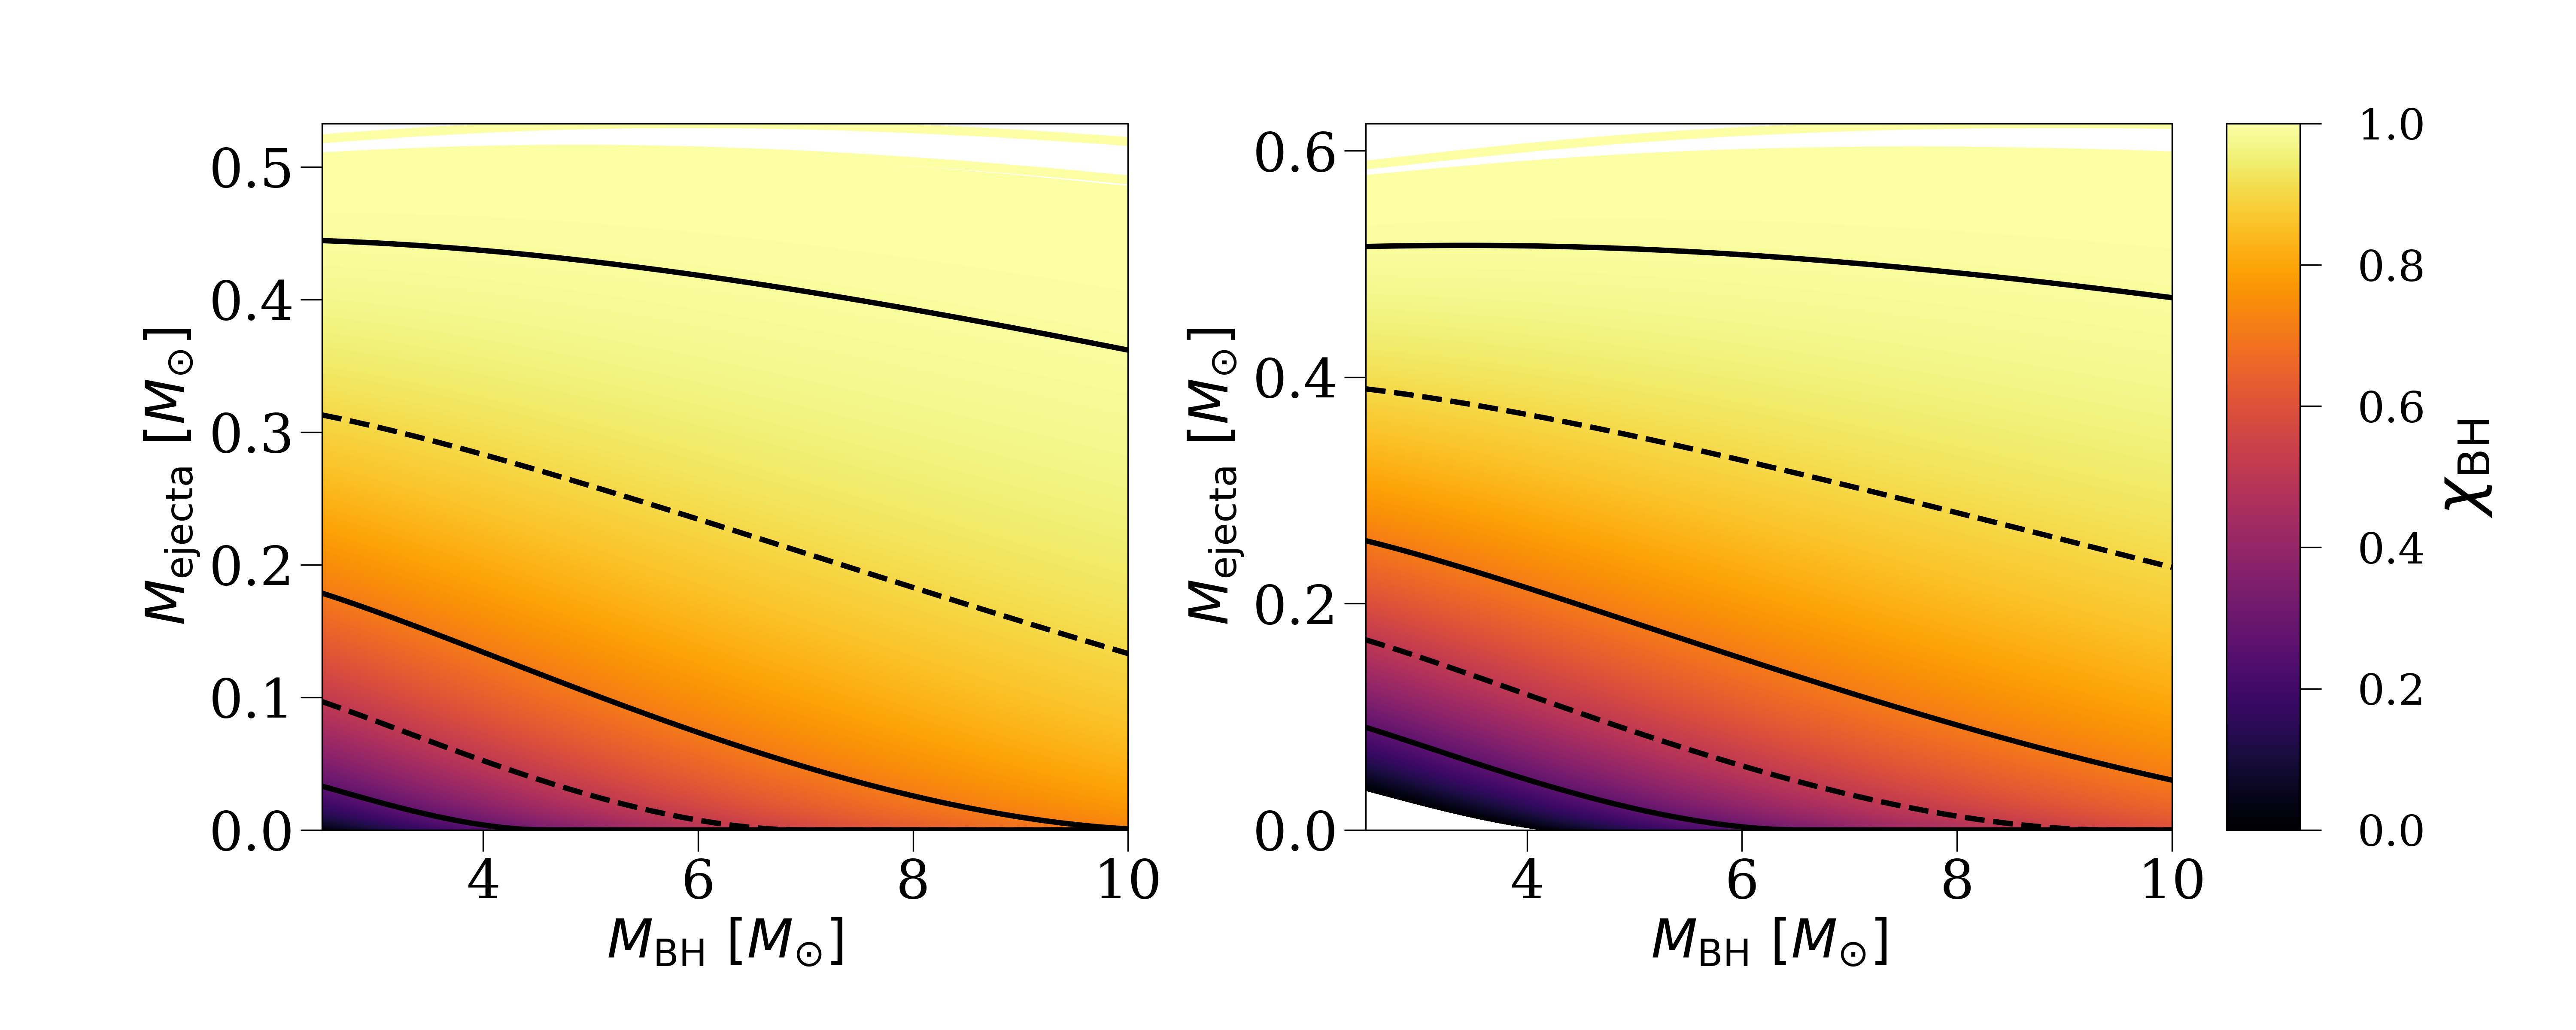
\includegraphics[width=1\textwidth]{../PlottingScripts/imagesUFDandRatios/PredictedMej.png} %CPUVsUncertaintySingleTogether.pdf}
%%    \caption{}
%%%    The number of binaries found of the target population  $N_{\mathrm{T}}$ as a function of the total number of binaries $N_{\text{binaries}}$ sampled for the traditional sampling method (gray dashed line) and the sampling method presented in this study (solid colored line). The four different panels show the simulations for each of the four target subpopulations. In each panel the duration of the exploratory phase is shown with a hashed gray area.  In the background the standard Poisson fractional uncertainties  of $0.3, 1$ and $3\%$ are shown with a dashed line.  } 
%%    \label{fig:PredictedMej}
%%\end{figure*}
%%%
%
%
%
%\subsubsection{Role of BH--NS compared to NSNS }
%\begin{itemize}
%	\item drake formula for rate of candidate 
%\end{itemize}
%
%\begin{equation}
%	\mathcal{R}_{\rm{candidates}} \approx \mathcal{R}_{\rm{merger}} \times f_{\rm{merges \ in \ halo}} \times f_{\rm{enriches}}
%\end{equation}
%
%
%%
%
%\subsubsection{rates of BH--NS candidates versus NSNS candidates }
%Table~\ref{tab:summary-simulations} summarizes the results from our binary population synthesis simulations focusing on the candidate systems that can enrich UFD galaxies from the different models simulated in this paper. The weight quoted in the table represent the number of candidate systems expected to form out of $10^6$ binaries drawn from the birth distributions as described in Section~\ref{sec:method}. 
%The weight  of BH--NS candidates in our \fiducial model is \fexplTwo, \EffExplTwo and   \EffRefTwo  for respectively assuming a black hole spin of $ \chi_{\rm{bh}} = 1, \chi_{\rm{bh}} = 0.5, $ and $\chi_{\rm{bh}} = 0$. 
%%The first column shows the physical models simulated in this work, where we show the  the different BH--NS simulations and the results for our \fiducial NSNS simulation for comparison.
%%The 2nd -- 4th columns show the total weight of the candidate systems in our simulation, which are defined as all the BH--NS or NSNS mergers that merge well within a halo with mass of $M \approx 10^9 \, M_{\odot}$ $(10^8 \, M_{\odot})$, with$ r_{\rm{vir}} \approx 4.6 \rm{kpc}$ $( \approx 1.3 \rm{kpc})$ with redshift $ z = 6 $ ( $ z =  10 $). Where the different columns represent different assumptions for the spin of the black hole in the $BH--NS$ binary of $\chi_{\rm{bh}} = 1, \chi_{\rm{bh}} = 0.5, $ and $\chi_{\rm{bh}} = 0$. 
% 
% 
 %%% TABLE
%\begin{table*} %{Summary of Adaptive Importance Sampling method results \\}
%\centering
%\label{tab:comparison2}
%\begin{tabular}{|l|c|c|c|c|c|c|c|}
%\hline
%\hline
%  Model		    &   weight candidates   &   weight   candidates  		&    weight  candidates  &  weight  all    & Fraction &   $\#$ candates /   	\\
%    &    $\chi_{\rm{bh}}=1$   &  $\chi_{\rm{bh}}=0.5$ 		&   $\chi_{\rm{bh}}=0$   &    &  &    $\#$ all mergers  	\\ \hline 
%NSNS \fiducial    &  \fexplOne  & \EffExplOne  & \EffRefOne & \NxMCOne   & \NxAISOne & \gainOne  \\ \hline
%BH--NS  \fiducial   &  \fexplTwo  & \EffExplTwo  & \EffRefTwo & \NxMCTwo   & \NxAISTwo & \gainTwo  \\ %\hline
%BH--NS   $Z=0.002$   &  \fexplThree  & \EffExplThree & \EffRefThree & \NxMCThree   & \NxAISThree & \gainThree  \\ %\hline
%BH--NS reduced kick  &  \fexplFour  & \EffExplFour  & \EffRefFour & \NxMCFour   & \NxAISFour & \gainFour  \\
% BH--NS $\alpha =0.1$       &  \fexplFive  & \EffExplFive  & \EffRefFive & \NxMCFive   & \NxAISFive & \gainFive  \\
%  BH--NS $\alpha =10$  &  \fexplSix  & \EffExplSix  & \EffRefSix & \NxMCSix   & \NxAISSix & \gainSix  \\ 
%  BH--NS Fryer \texttt{RAPID}  &  \fexplSeven & \EffExplSeven  & \EffRefSeven & \NxMCSeven   & \NxAISSeven & \gainSeven  \\  
% \hline
%\end{tabular}
%\caption{The total weight (i.e. number) of double compact objects formed out of $10^6$ binaries simulated in each model. The total weight is derived from combining the probability of occuring of each binary in the simulation and equals `the number of binaries out of the total simulation`.  A description of the models is given in Section \ref{subsec:method-COMPASmodel}.  The 2nd to 4th column give the total weight of double compact objects that merges well within the virial radius of  a halo with mass $10^9 M_{\odot} \ (r_{\rm{vir}}   = 4.6 \, \rm{kpc})$ at $z \approx 6$. In parenthesis the total weight of the systems is shown that merge within a halo of mass   $10^8 M_{\odot} $ $ (r_{\rm{vir}}   = 1.3 \, \rm{kpc})$ at $z \approx 10$. The fifth column shows the total weight of all double compact object systems that merge within a Hubble time, and the sixth column shows the fraction  of all double compact object mergers that is a candidate system. The last column shows the total number of binaries out of $10^6$ that evolved to a candidate and to all double compact object systems.  }
%\label{tab:summary-simulations}
%\end{table*} 

\subsubsection{properties in vsys and time frame, and eccentricity versus separation frame }
%
%\begin{figure*}
%	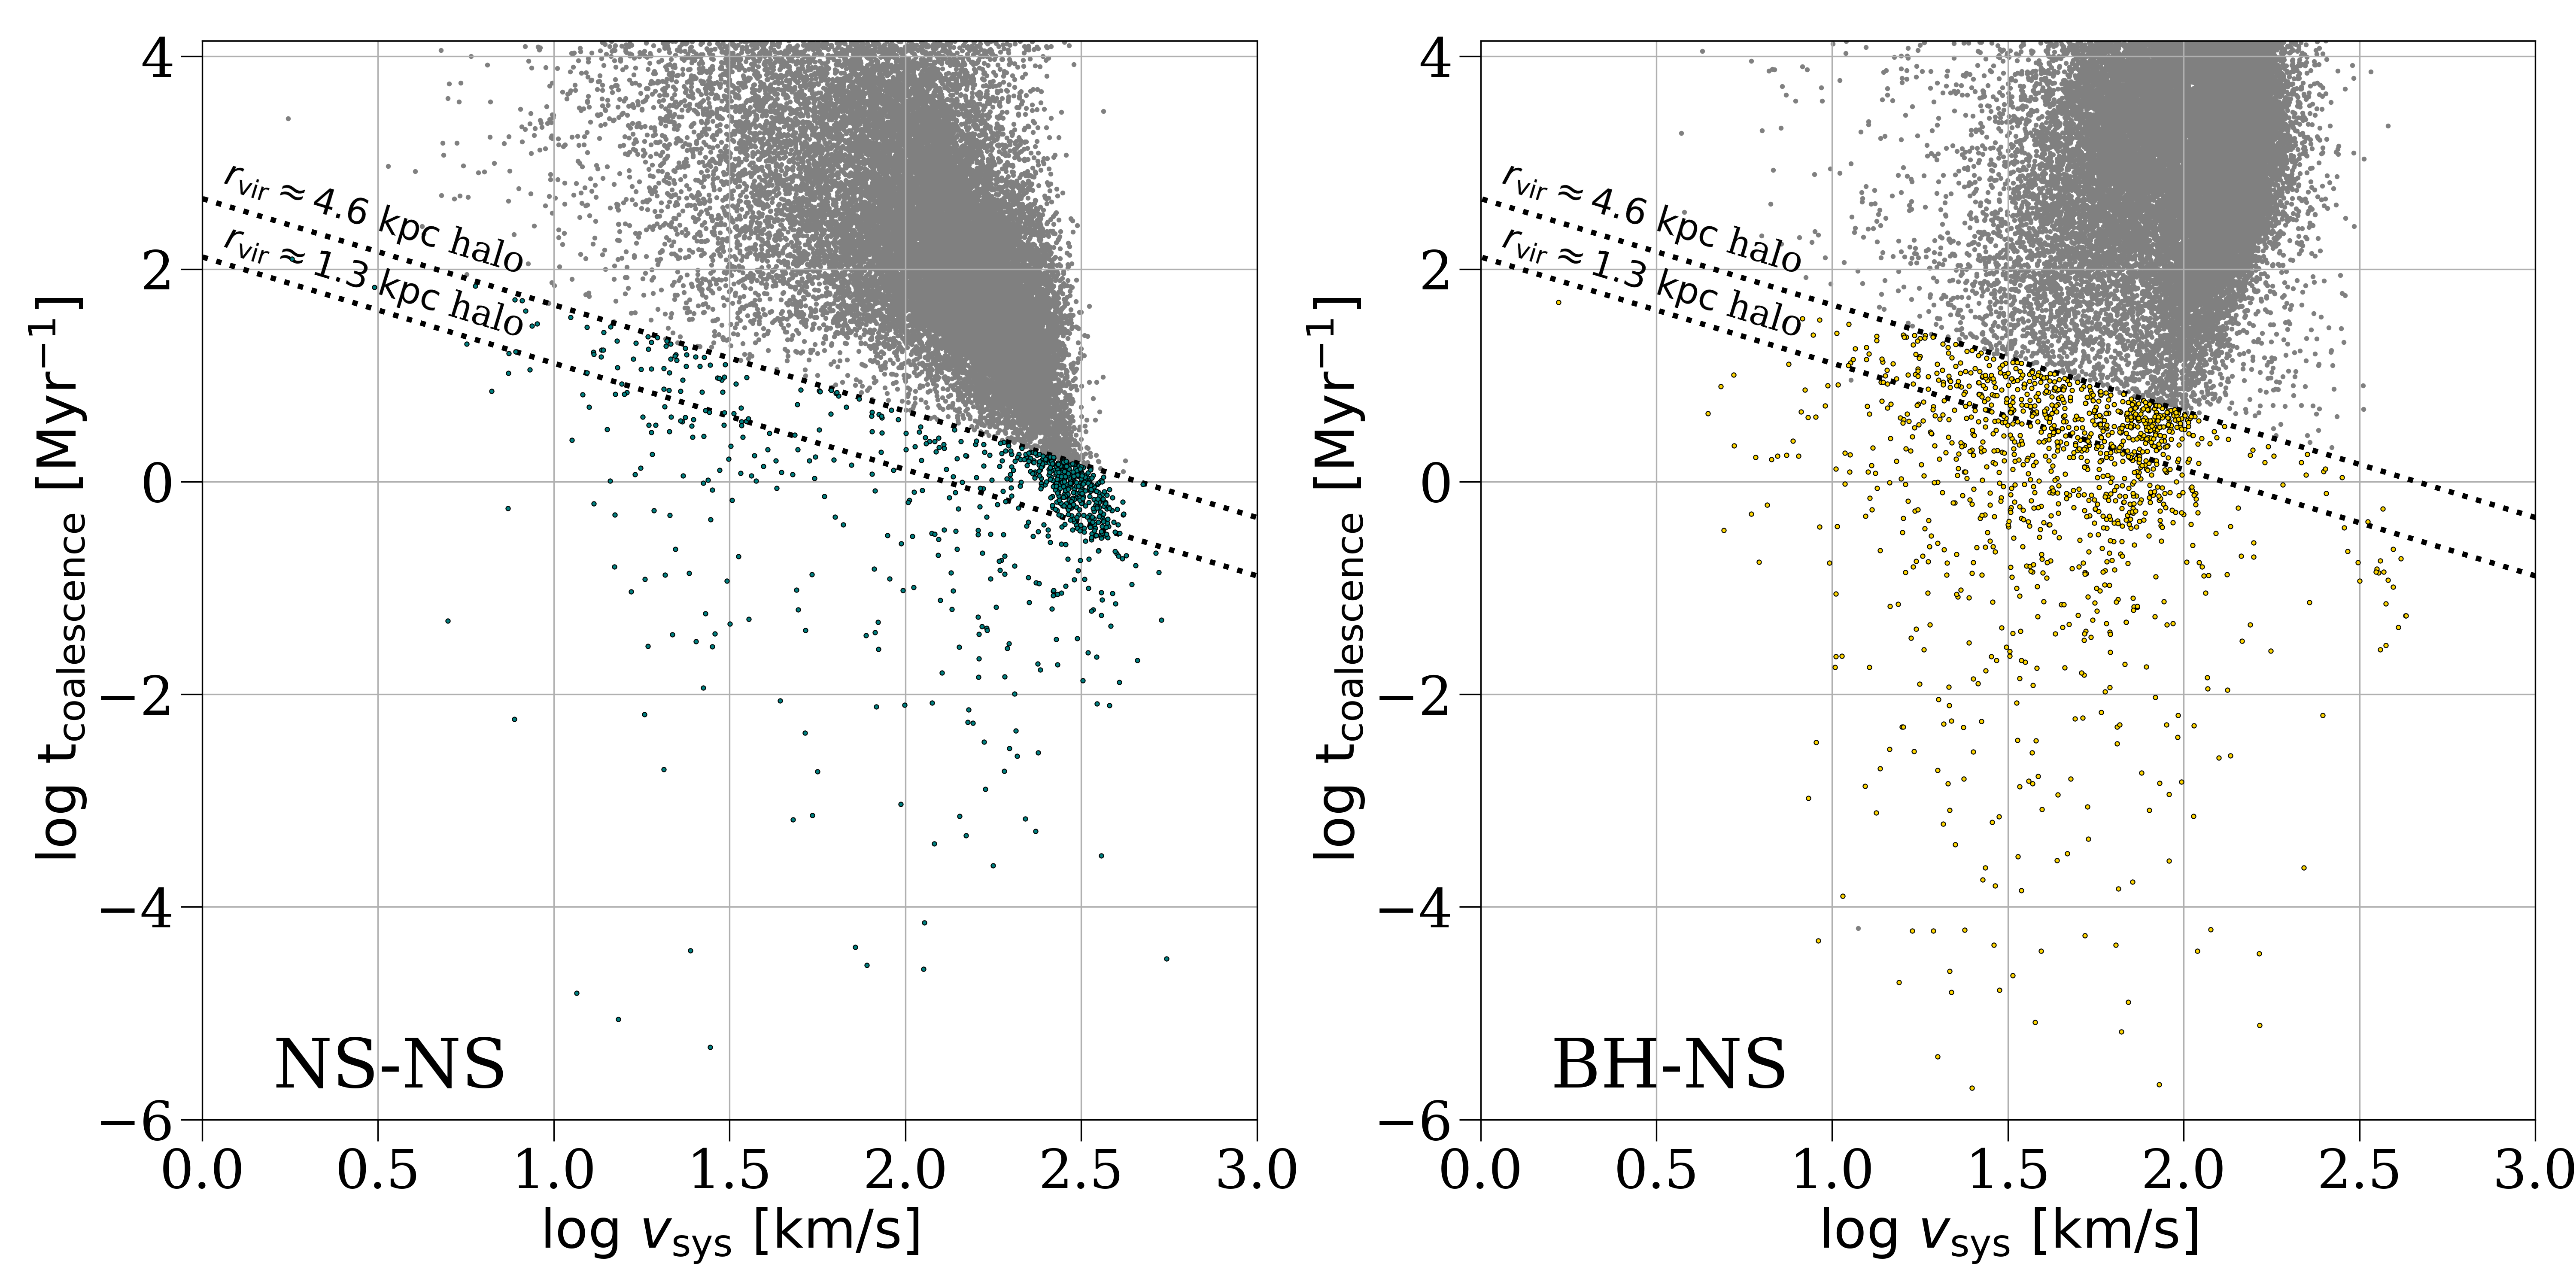
\includegraphics[width=1\textwidth]{../PlottingScripts/imagesUFDandRatios/scatterCandidates_Xeff.pdf} %CPUVsUncertaintySingleTogether.pdf}
%    \caption{The systematic velocity of the binary system versus the coalescence time, at the moment the double compact object formed. \textbf{[left panel:] } NSNS mergers and candidates,   \textbf{[right panel:] } BH-NS mergers and candidate systems when assuming a high spinning \ac{BH} with  $\chi_{\rm{bh}} = 0.97$. In grey all double compact object mergers of that modeled population. A small subset of those mergers, merges well within the radius of a halo of $10^9 M_{\odot} \ (r_{\rm{vir}}   = 4.6 \, \rm{kpc})$ at $z \approx 6$ or a halo of mass   $10^8 M_{\odot} $ $ (r_{\rm{vir}}   = 1.3 \, \rm{kpc})$ at $z \approx 10$.   Dotted lines indicate the maximum $v_{\rm{sys}} \times t_{\rm{coalescence}}$ that is needed to merge within those halos}
%    \label{fig:NbinariesVsNHits}
%\end{figure*}


%
%\begin{figure*}
%	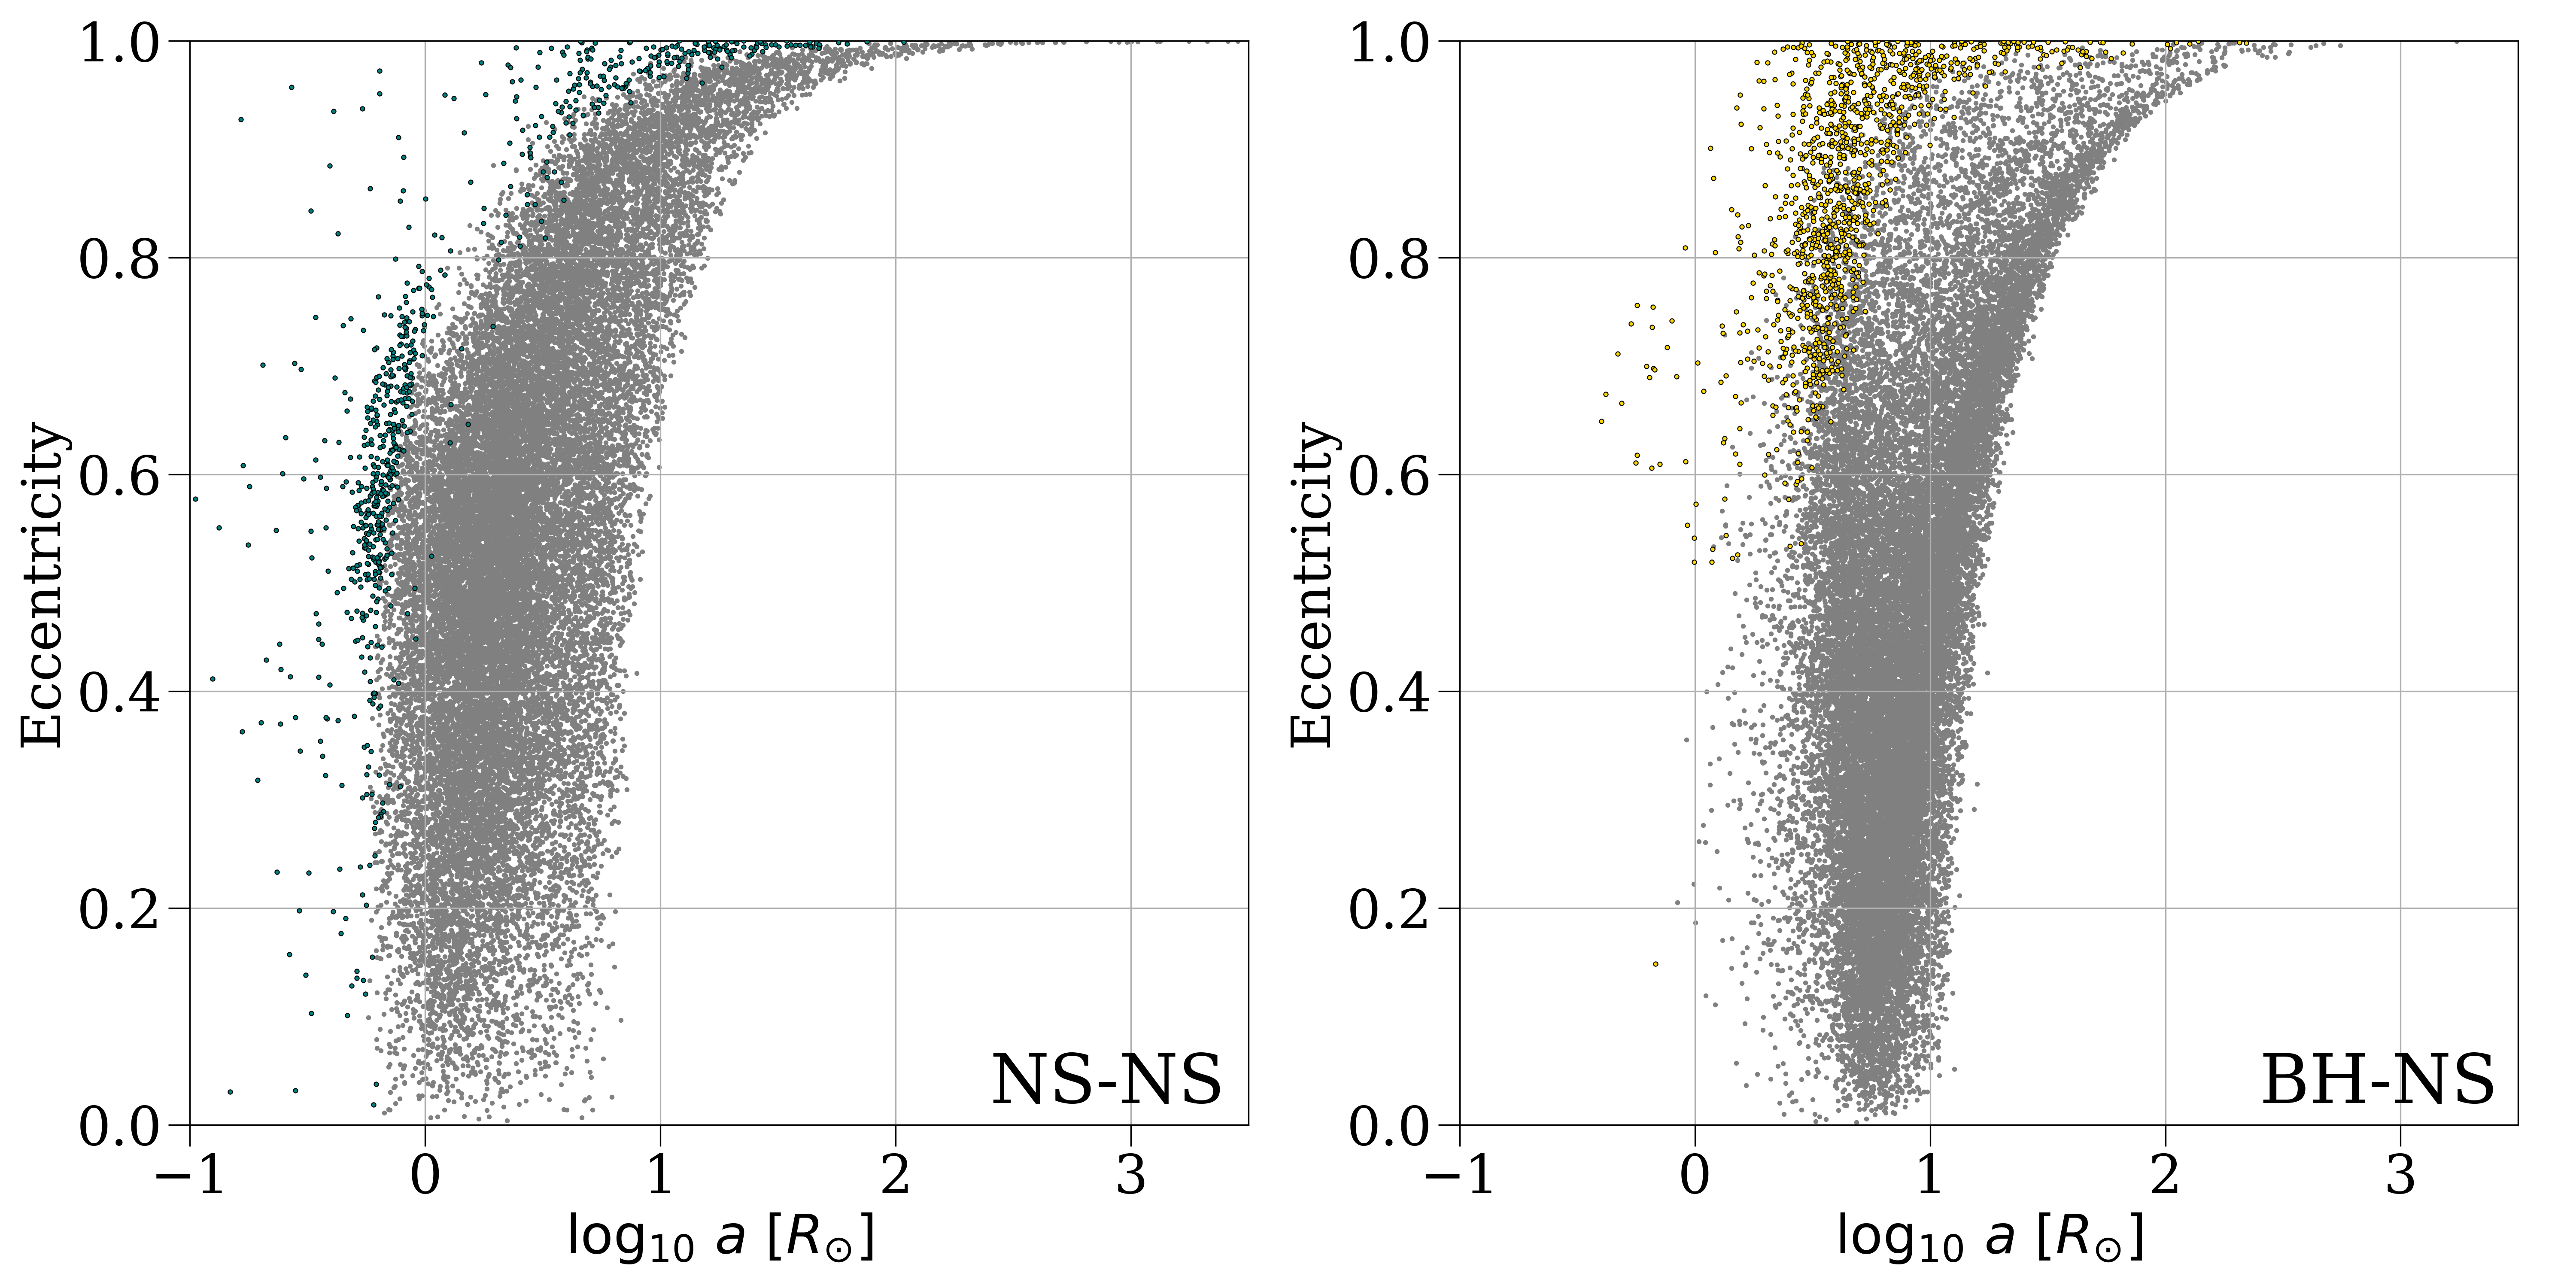
\includegraphics[width=1\textwidth]{../PlottingScripts/imagesUFDandRatios/scatterCandidates_Xeff_II.pdf} %CPUVsUncertaintySingleTogether.pdf}
%    \caption{The separation  of the binary system versus the eccentricity at the moment the double compact object formed. The systems that merge well within the halo of an UFD are coloured with blue or yellow.  \textbf{[left panel:] } NSNS mergers and candidates,   \textbf{[right panel:] } BH-NS mergers and candidate systems when assuming a high spinning \ac{BH} with  $\chi_{\rm{bh}} = 0.97$. In grey all double compact object mergers of that modeled population.}
%    \label{fig:NbinariesVsNHits}
%\end{figure*}


\subsubsection{properties of the candidate systems}
\begin{itemize}
	\item systematic velocities
	\item natal kick properties
	\item \ac{BH} vs \ac{NS} forms first  (do this here or in formation channel discussion) 
	\item traveled distance
\end{itemize}
%
%\begin{figure*}
%	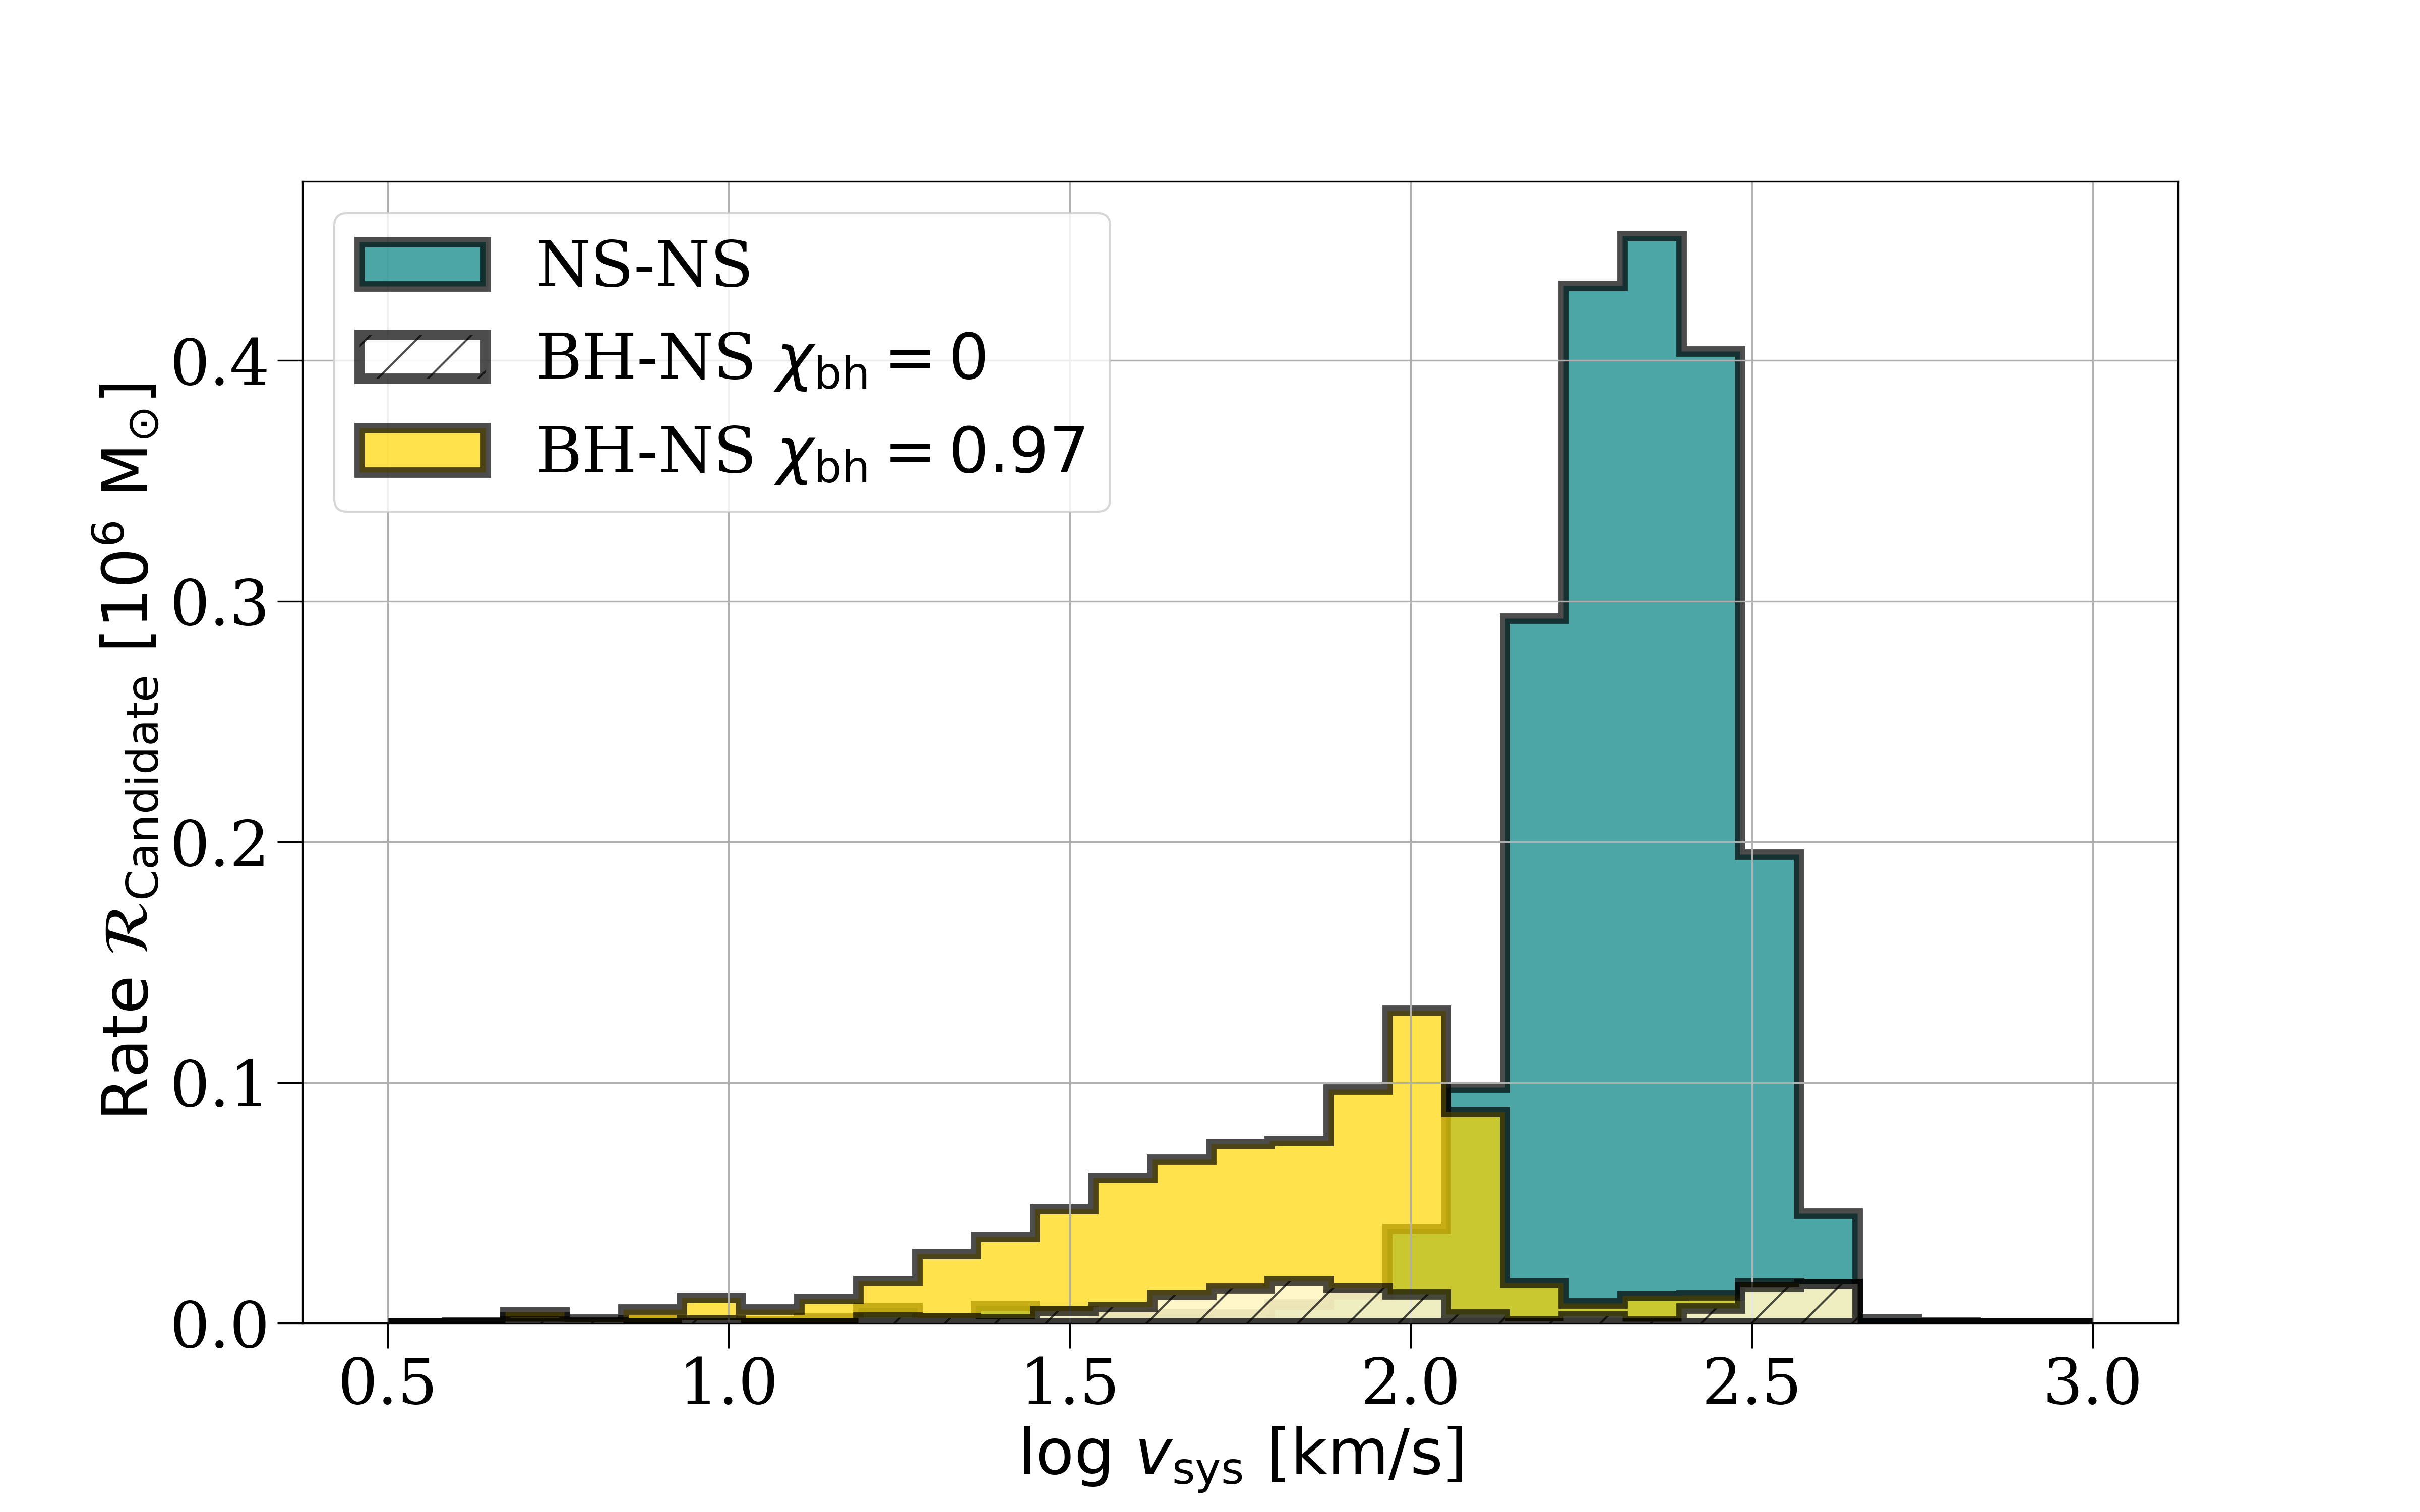
\includegraphics[width=1\columnwidth]{../PlottingScripts/imagesUFDandRatios/tsystematicPDF.pdf} %CPUVsUncertaintySingleTogether.pdf}
%    \caption{Distribution function of the systematic velocity of the candidate binaries after the second supernova. In blue the distribution for NSNS candidates are shown, whereas in yellow the distribution for BH--NS systems is shown assuming a black hole spin of  $\chi_{\rm{bh}} = 0.97$ (where the hatched  area shows the distribution of BH--NS candidates if $\chi_{\rm{bh}} = 0$. It is clearly visible that NSNS and BH--NS candidates have a distinct distribution function for $v_{\rm{sys }}$ with BH--NS having overall smaller systematic velocities}
%%    The number of binaries found of the target population  $N_{\mathrm{T}}$ as a function of the total number of binaries $N_{\text{binaries}}$ sampled for the traditional sampling method (gray dashed line) and the sampling method presented in this study (solid colored line). The four different panels show the simulations for each of the four target subpopulations. In each panel the duration of the exploratory phase is shown with a hashed gray area.  In the background the standard Poisson fractional uncertainties  of $0.3, 1$ and $3\%$ are shown with a dashed line.  } 
%    \label{fig:NbinariesVsNHits}
%\end{figure*}
%


%\begin{figure*}
%	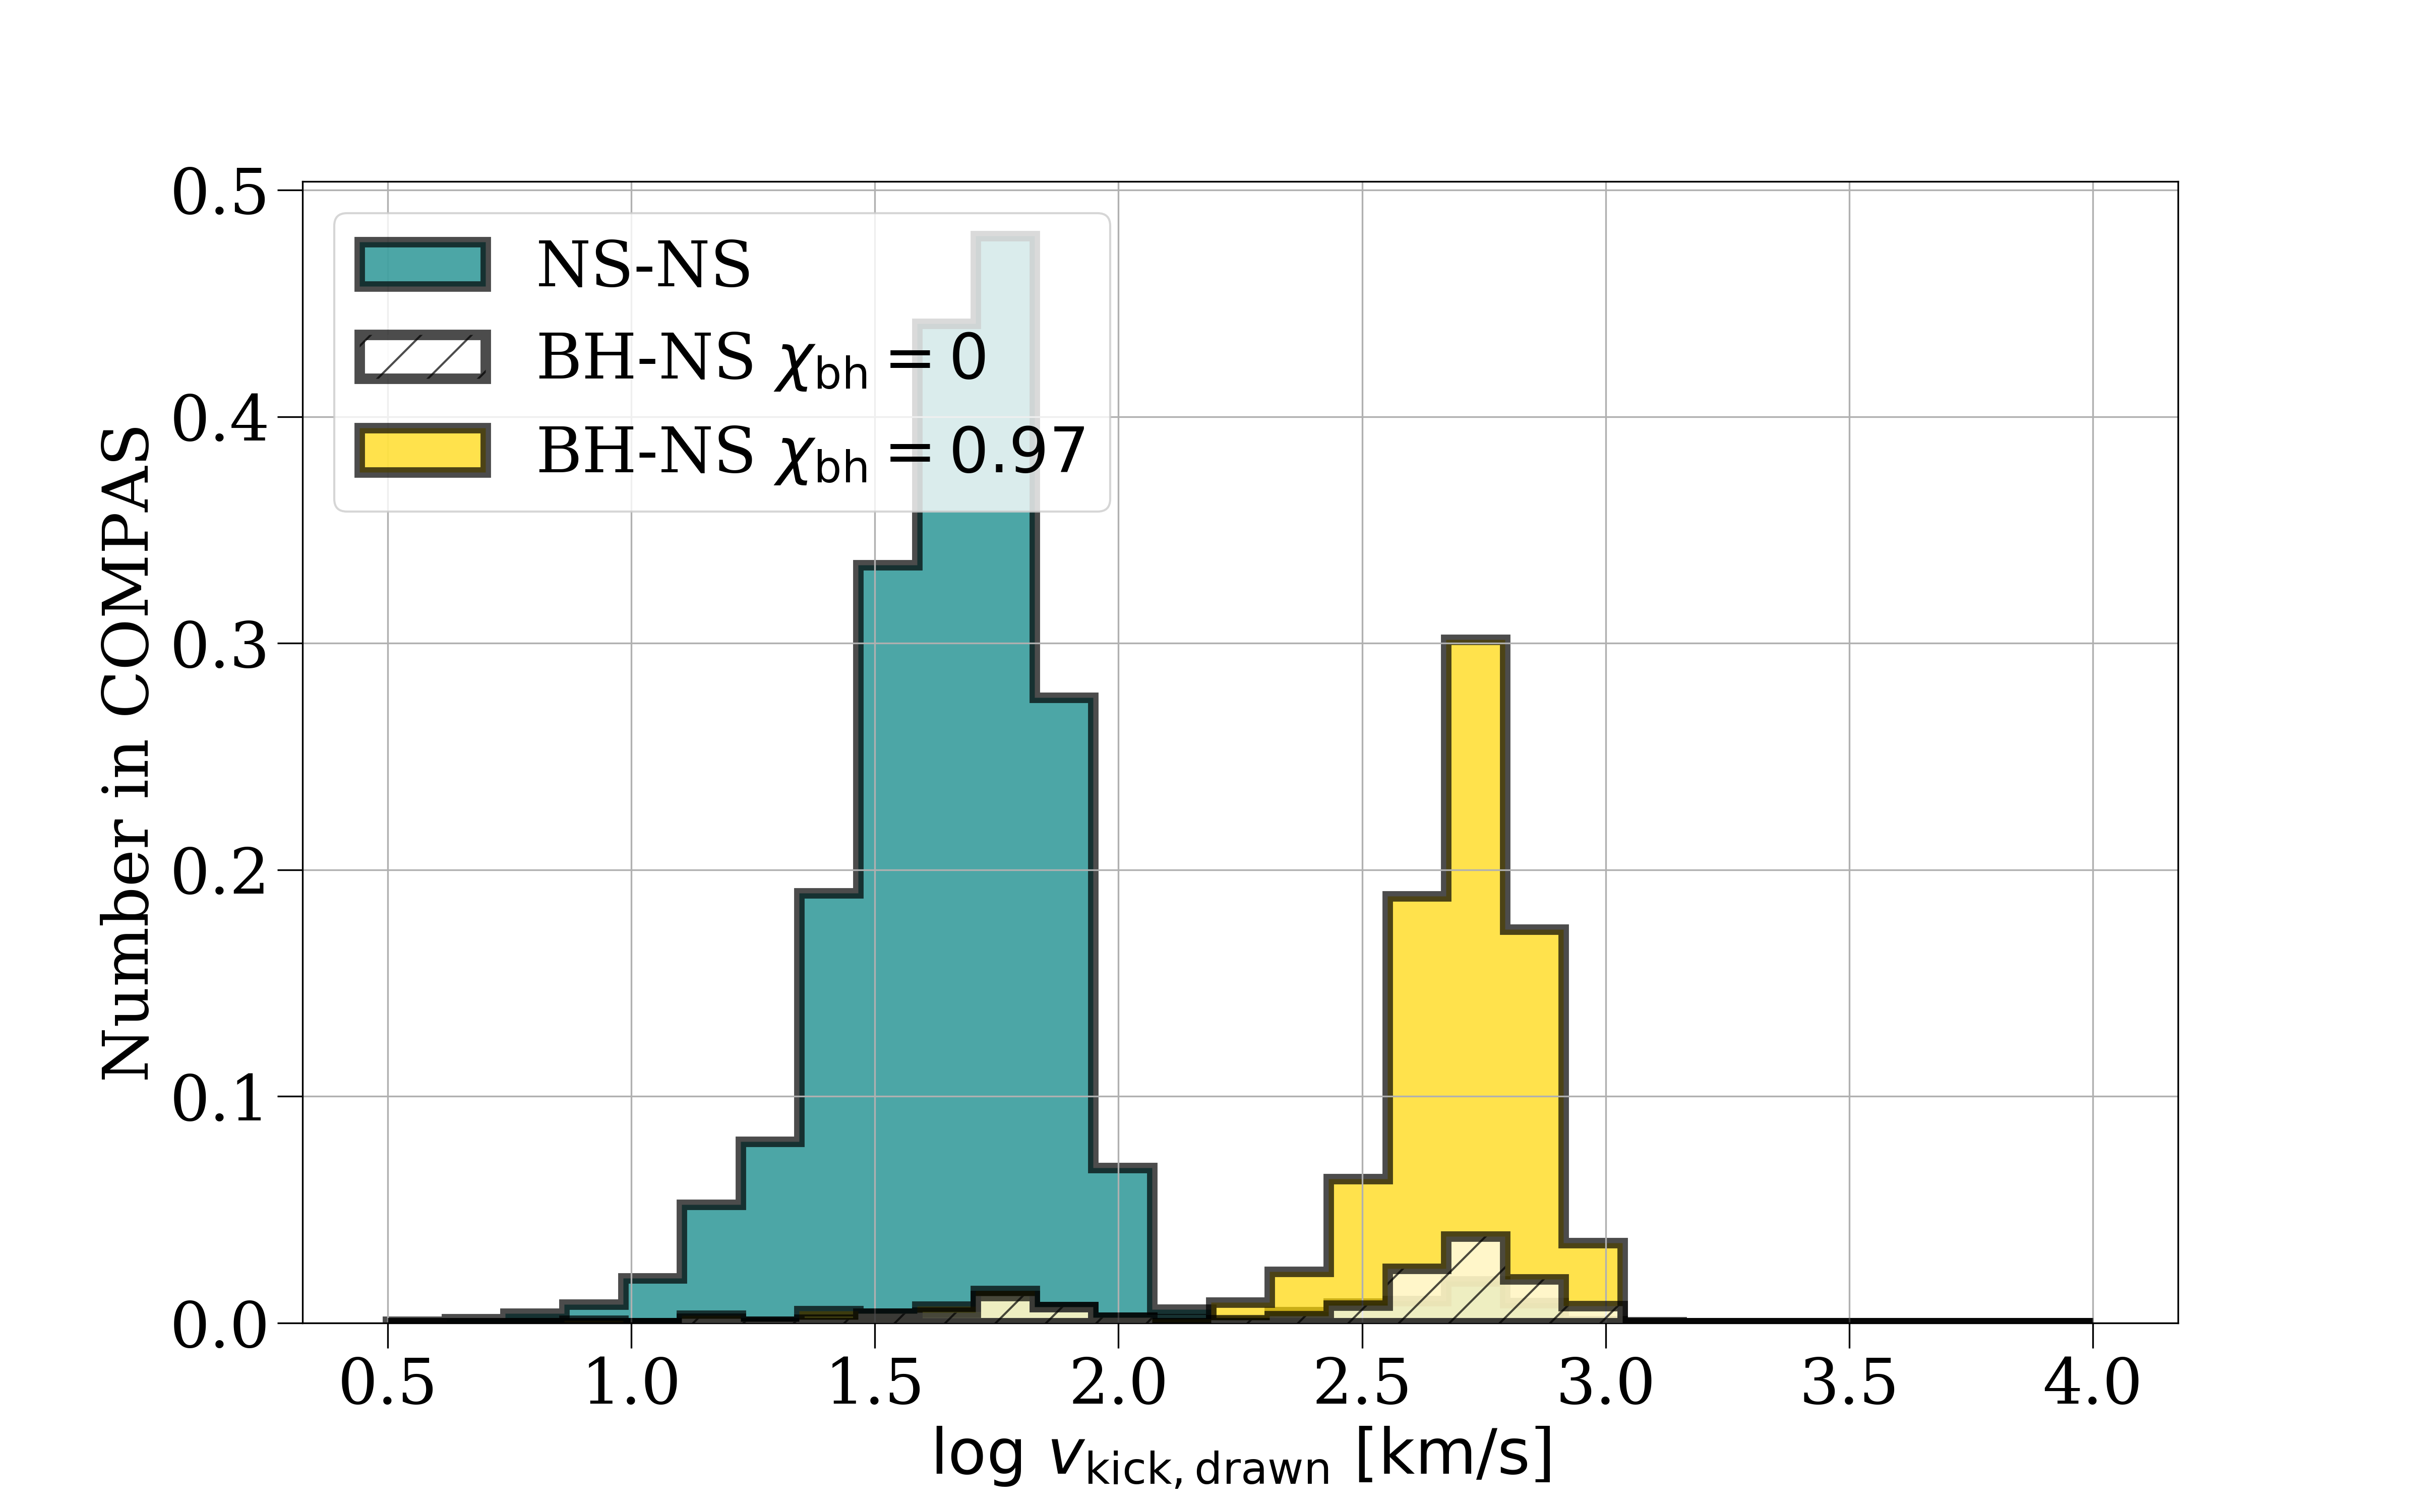
\includegraphics[width=1\columnwidth]{../PlottingScripts/imagesUFDandRatios/drawnKickVelocityPDF.pdf} %CPUVsUncertaintySingleTogether.pdf}
%    \caption{Distribution function of the drawn kick velocity magnitudes of the candidate binaries after the second supernova. In blue the distribution for NSNS candidates are shown, whereas in yellow the distribution for BH--NS systems is shown assuming a black hole spin of  $\chi_{\rm{bh}} = 0.97$ (where the hatched  area shows the distribution of BH--NS candidates if $\chi_{\rm{bh}} = 0$. It is clearly visible that NSNS and BH--NS candidates have a distinct distribution function for $v_{\rm{k }}$ with BH--NS having overall larger drawn kick velocities.}
%%    The number of binaries found of the target population  $N_{\mathrm{T}}$ as a function of the total number of binaries $N_{\text{binaries}}$ sampled for the traditional sampling method (gray dashed line) and the sampling method presented in this study (solid colored line). The four different panels show the simulations for each of the four target subpopulations. In each panel the duration of the exploratory phase is shown with a hashed gray area.  In the background the standard Poisson fractional uncertainties  of $0.3, 1$ and $3\%$ are shown with a dashed line.  } 
%    \label{fig:NbinariesVsNHits}
%\end{figure*}
%

%%
%\begin{figure*}
%		\includegraphics*[width=1\columnwidth]{../PlottingScripts/imagesUFDandRatios/traveldistancePDF_Xeff0_97.pdf}
%		\includegraphics*[width=1\columnwidth]{../PlottingScripts/imagesUFDandRatios/traveldistanceCDF_Xeff0_97.pdf}
%%
%%    \label{fig:RateCandidateEnriching}
%%\end{figure*}
%%%
%%%
%%\begin{figure*}
%		\includegraphics*[width=1\columnwidth]{../PlottingScripts/imagesUFDandRatios/traveldistancePDF_Xeff0_0.pdf}
%		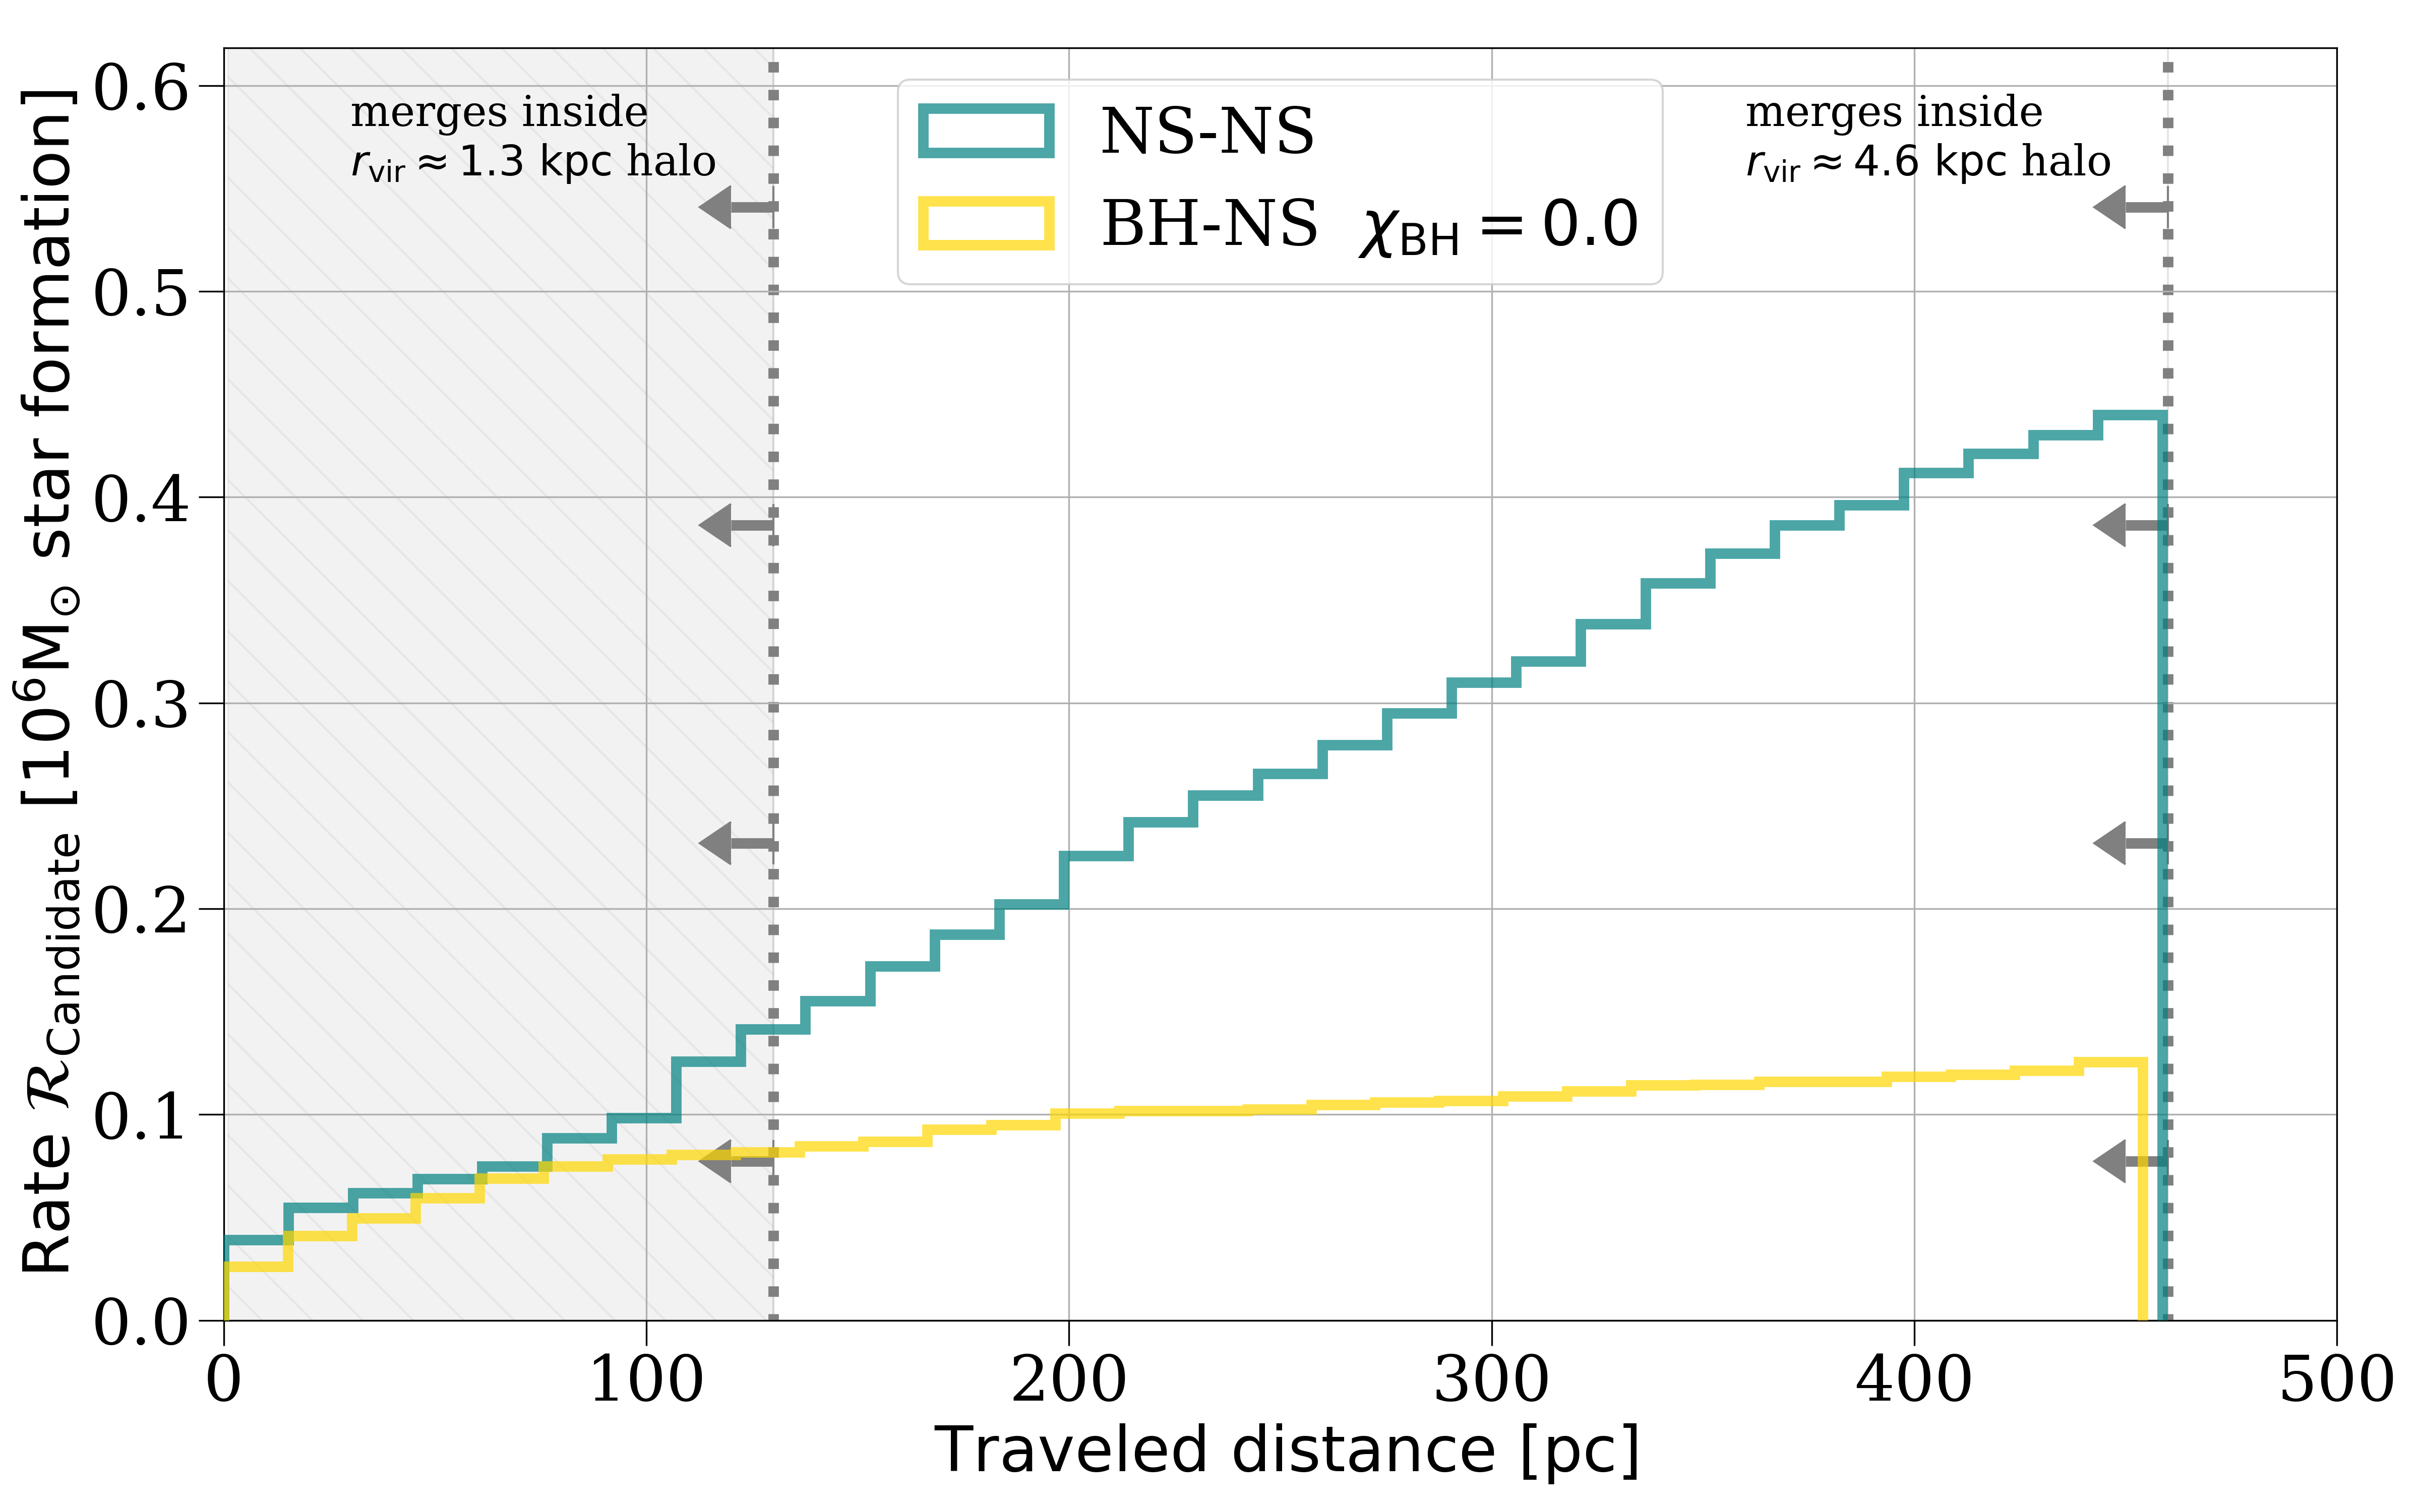
\includegraphics[width=1\columnwidth]{../PlottingScripts/imagesUFDandRatios/traveldistanceCDF_Xeff0_0.pdf}
%    \caption{\textbf{Left panel:} distribution function and \textbf{right panel:} cumulative distribution function of the travelled distance of the candidate binaries between the second \ac{SN}  and the merger. In blue the distribution for NSNS candidates are shown, whereas in yellow the distribution for BH--NS systems is shown. \textbf{Upper panel:}  assuming a black hole spin of  $\chi_{\rm{bh}} = 0.97$. \textbf{lower panel:} the same but now assuming BH--NS candidates have a black hole with spin $\chi_{\rm{bh}} = 0$.  BH--NS candidate rates are similar for both assumed halos if the black holes have a high spin, whereas if black holes have negligible spin, the BH--NS become mostly important for lower mass halos. } 
%    \label{fig:RateCandidateEnriching}
%\end{figure*}

%
\subsubsection{rates comparison with UFD galaxies}
%
%\begin{figure*}
%		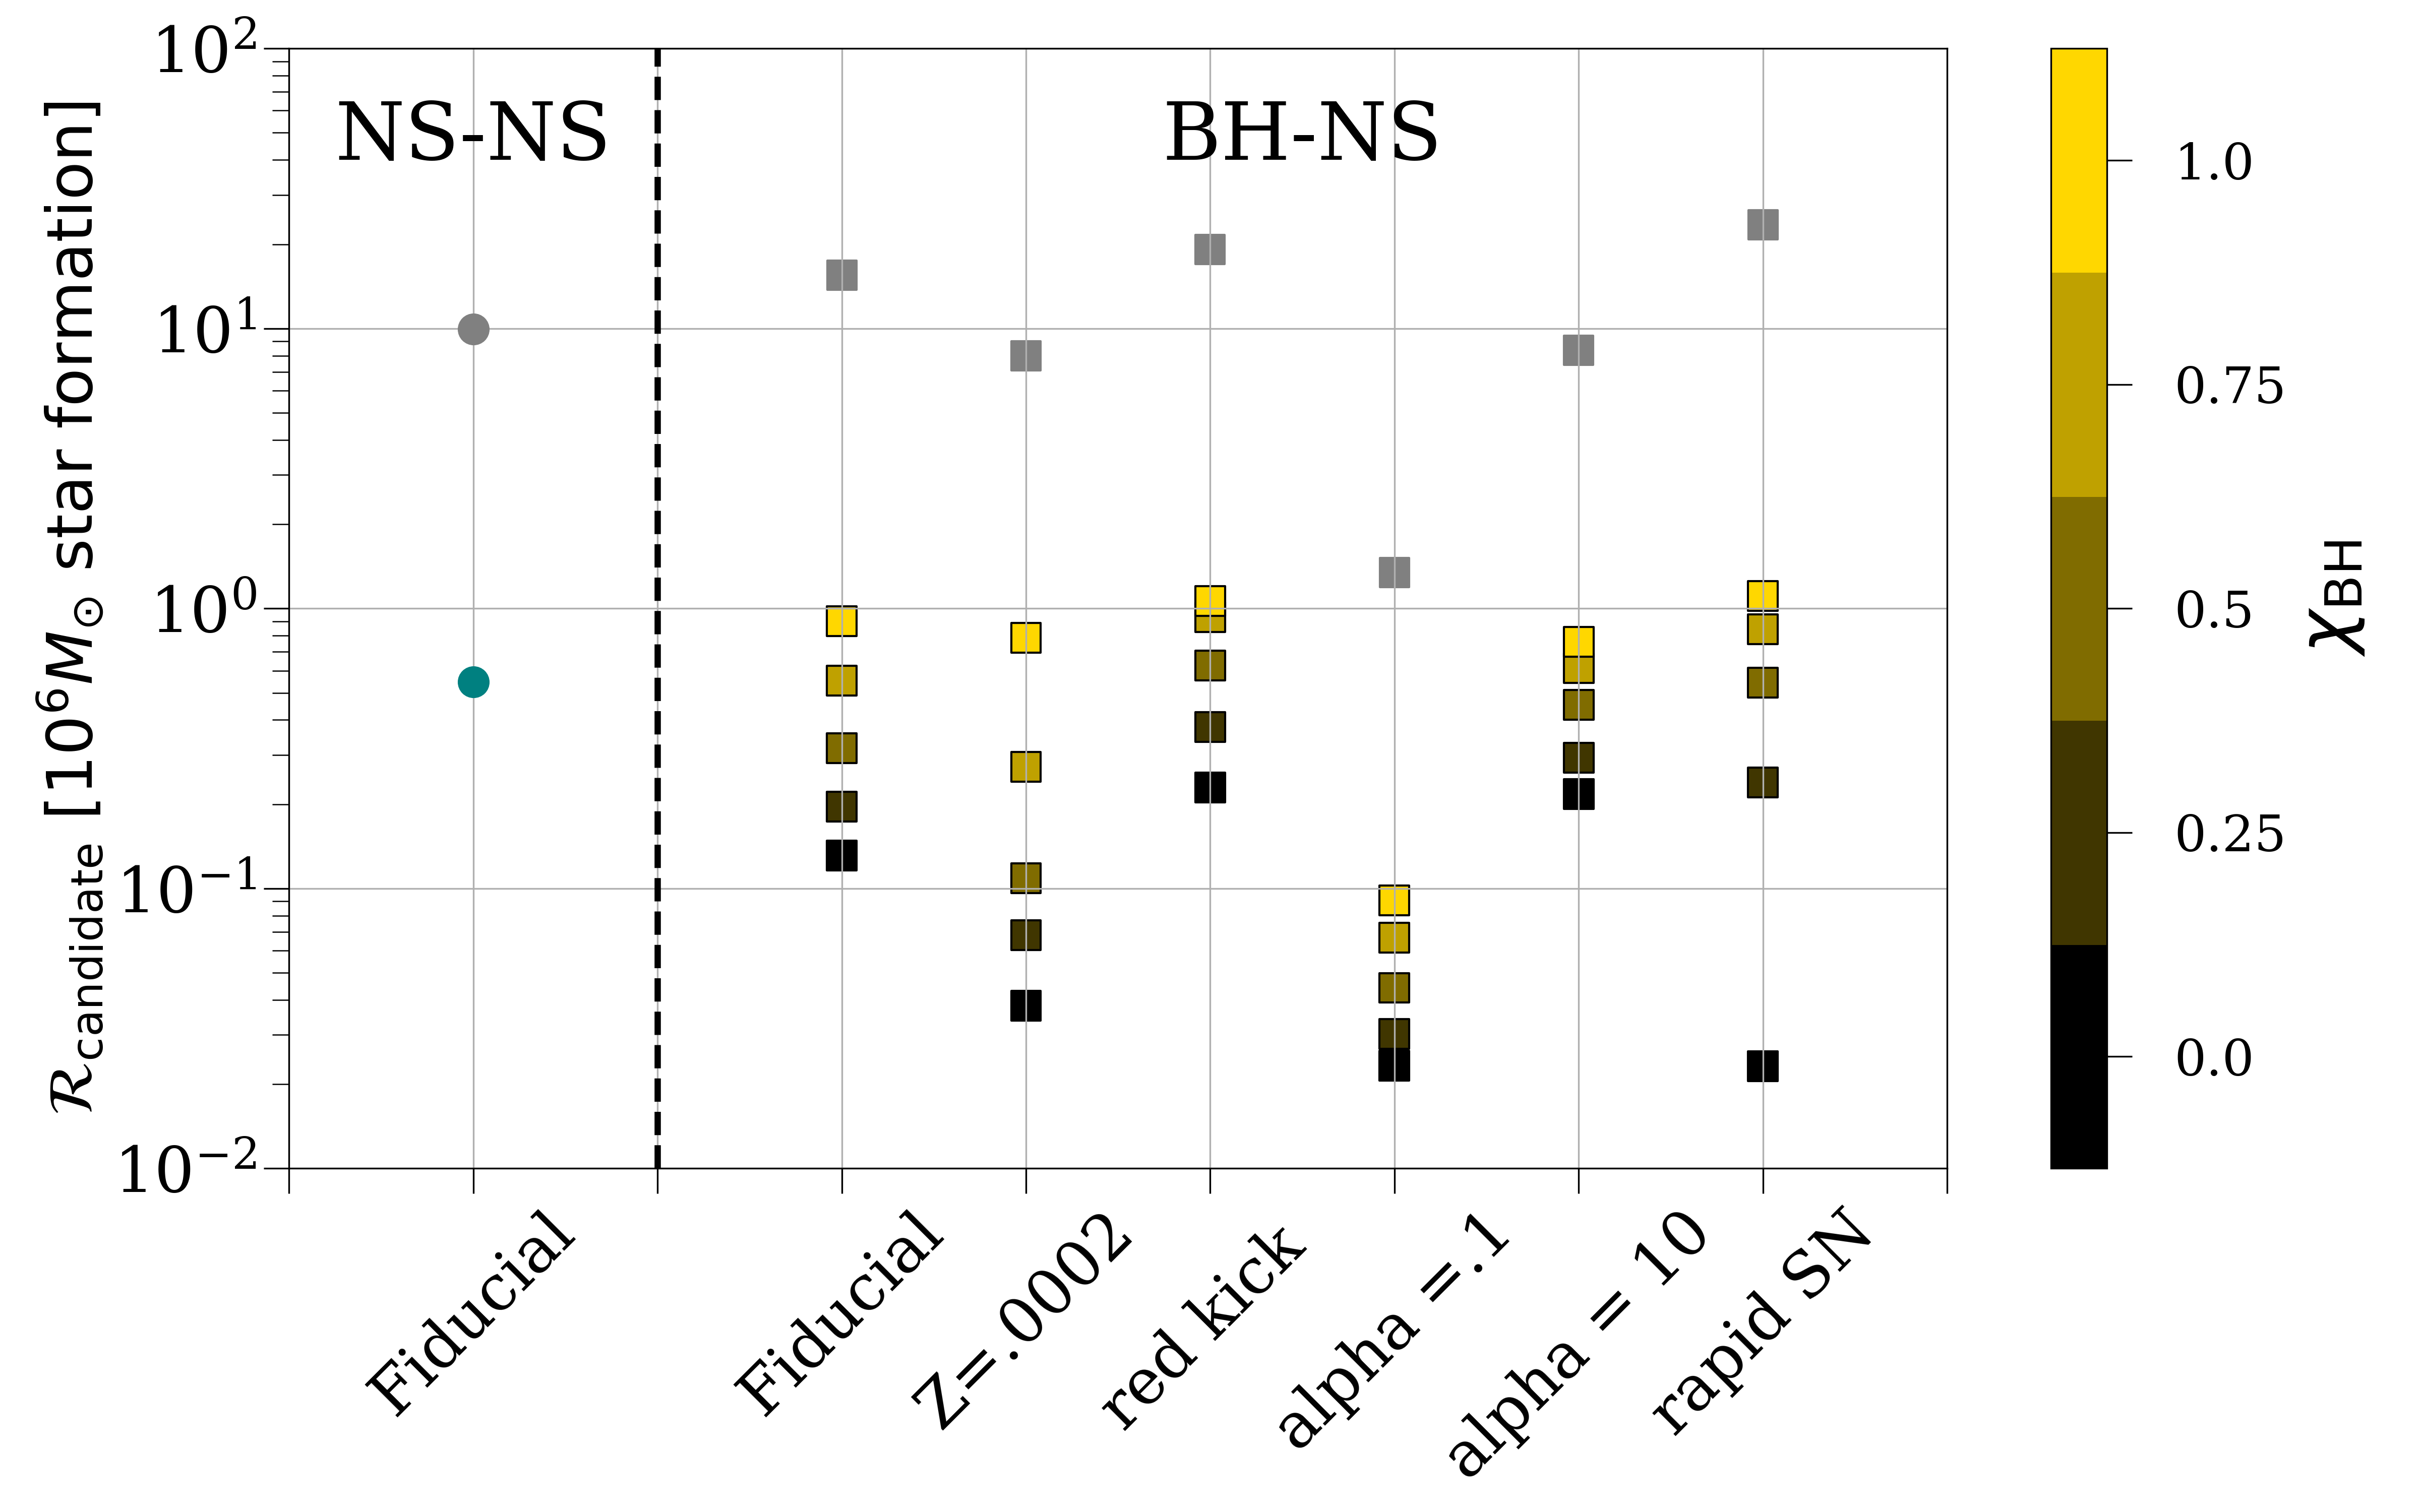
\includegraphics[width=1\textwidth]{../PlottingScripts/imagesUFDandRatios/RateUFDEnrichingMergers2.pdf}
%		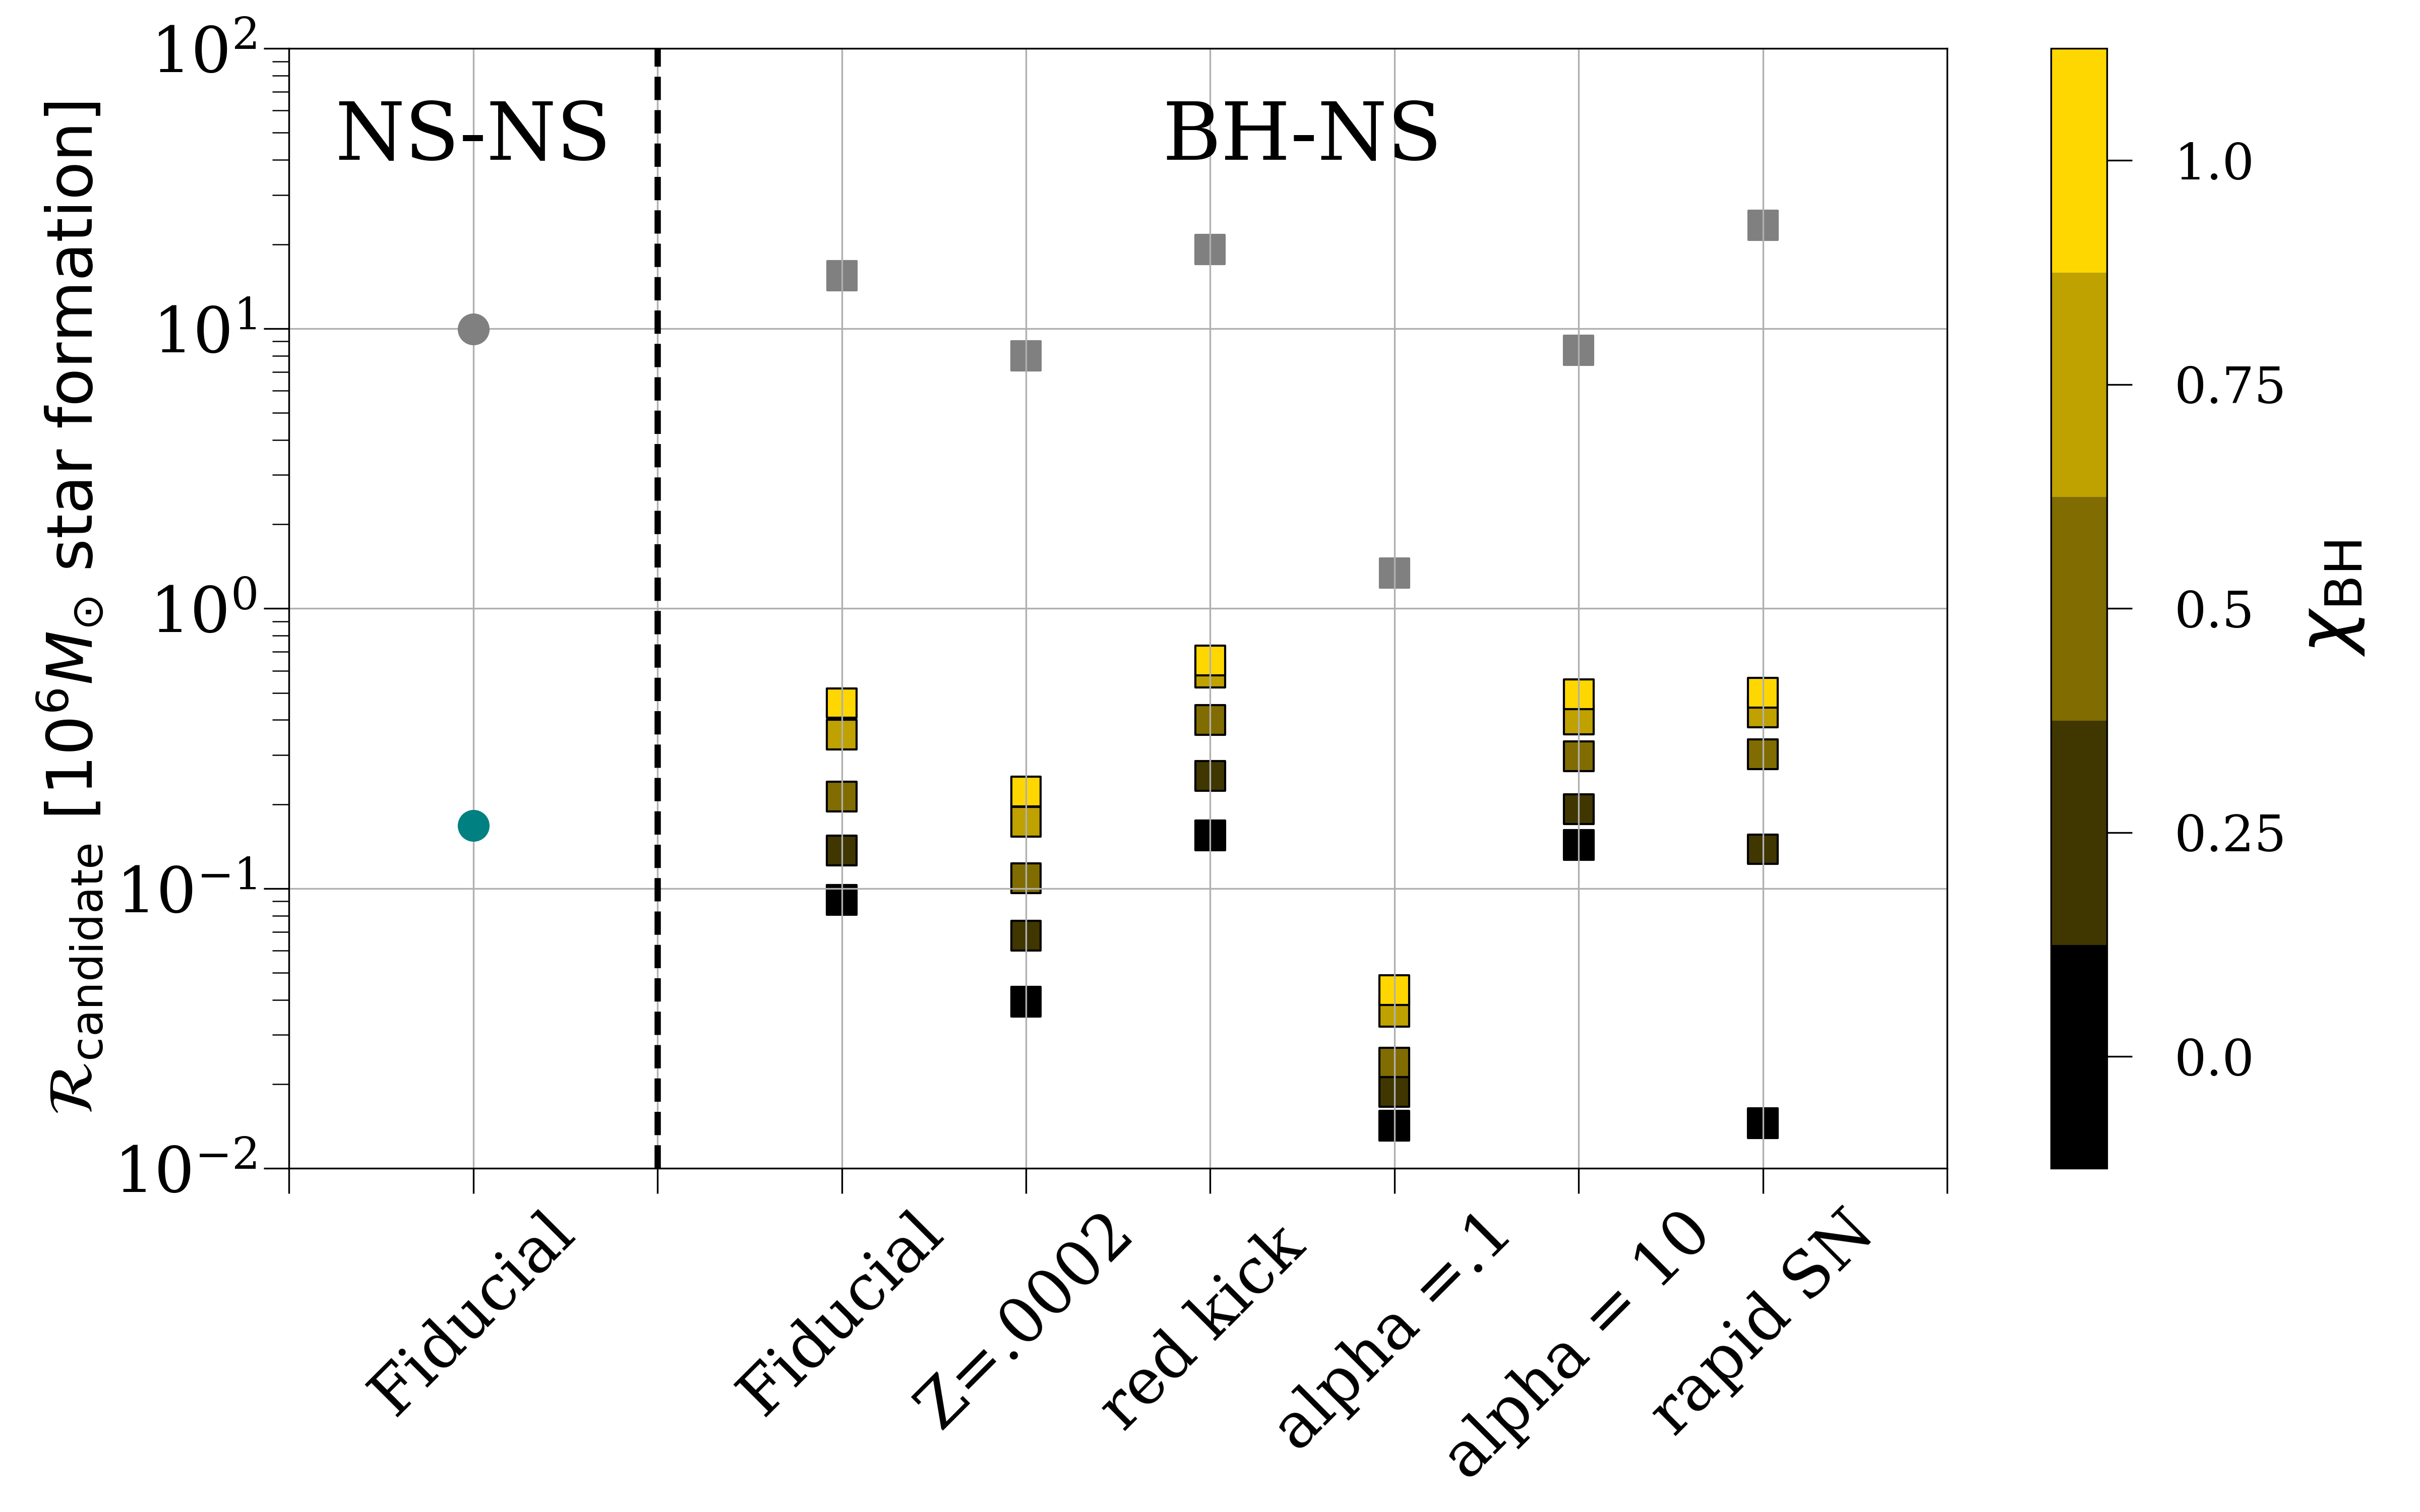
\includegraphics[width=1\textwidth]{../PlottingScripts/imagesUFDandRatios/RateUFDEnrichingMergers2_Rvir1_3.pdf}
%    \caption{ The formation rate of candidate  NSNS (first cirlce data point) and BH--NS (square data points) binaries. Each data point indicates the total rate of formation of candidate systems per $10^6 \ \rm{M}_{\odot}$ star formation. There are one circle and 6 squares which correspond to the one NSNS model and 6 BH--NS models studied here. In grey for each model the rate of all double compact mergers in a Hubble time is given. A fraction of those mergers, mergers well within the ultra-faint-dwarf galaxy, possibly makes r-processes  and merges fast enough to be able to explain the r-process enriched UFD. The rate of those candidate systems are shown with a coloured datapoint. For BH--NS candidate mergers the rate of candidate systems depends on the assumption for the black hole spin which is is shown with the colorbar} 
%    \label{fig:RateCandidateEnriching}
%\end{figure*}

%


%
\subsubsection{Evolutionary channels of the fast merging systems}
\label{sec:evolutionchannels}




\section*{Acknowledgements}


%Numerical computations were performed at Oakforest-PACS at Information Technology Cen- ter of the University of Tokyo, Cray XC50 at CfCA of National Astronomical Observatory of Japan, Cray XC40 at Yukawa Institute for Theoretical Physics of Kyoto University, and Sakura and Cobra clus- ters at Max Planck Computing and Data Facility



Lieke for all her help on binary stellar evolution and gravitational waves, Mathieu for his help on  \ac{SN} and wind loss. 
Serena on her help on accretion onto compact objects , Debatri on Pulsars, Gus Beane with his help on galaxies. 
Griffin, Lokesh, Tom, Floris, Victoria, Miranda and Locke 

Carl Rodriguez on discussions on dynamical formation of \bhnsSingle mergers, Chris Fryer for discussions on the  \ac{SN} remnant mass prescription. Tulutov
Miranda, Locke and Victoria for help.

Facilities: ADS

Software: \\
\textsc{COMPAS}  \citep{stevenson2017formation, 2018MNRAS.477.4685B, 2018MNRAS.481.4009V},   \texttt{Python} available from \url{python.org}, matplotlib \citep{2007CSE.....9...90H},  \texttt{NumPy} \citep{2011CSE....13b..22V}, \texttt{ipython$/$jupyter} \citep{2007CSE.....9c..21P, kluyver2016jupyter} This paper used the \texttt{Astropy} library \citep{2018AJ....156..123A}.

 {\sc{SEOBNRv3}} and  {\sc{IMRPhenomPv2}}

%
%The Berger Time-Domain Group is supported in part by NSF grant AST-1714498 and NASA grant NNX15AE50G. G.H. thanks the LSSTC Data Science Fellowship Program, which is funded by LSSTC, NSF Cybertraining Grant \#1829740, the Brinson Foundation, and the Moore Foundation; his participation in the program has benefited this work. F.D.\ thanks the SAO REU program, funded in part by the National Science Foundation REU and Department of Defense ASSURE programs under NSF Grant no.\ AST-1852268 and by the Smithsonian Institution. V.A.V.\ acknowledges support by the National Science Foundation through a Graduate Research Fellowship.


This research has made use of data, software and/or web tools obtained from the \ac{GW} Open Science Center (\url{https://www.gw-openscience.org}), a service of LIGO Laboratory, the LIGO Scientific Collaboration and the Virgo Collaboration. LIGO is funded by the U.S. National Science Foundation. Virgo is funded by the French Centre National de Recherche Scientifique (CNRS), the Italian Istituto Nazionale della Fisica Nucleare (INFN) and the Dutch Nikhef, with contributions by Polish and Hungarian institutes.
%
%%%%%%%%%%%%%%%%%%%%%%%%%%%%%%%%%%%%%%%%%%%%%%%%%%
%
%%%%%%%%%%%%%%%%%%%% 




\bibliography{my_bib}{}
\bibliographystyle{aasjournal}







%% This command is needed to show the entire author+affiliation list when
%% the collaboration and author truncation commands are used.  It has to
%% go at the end of the manuscript.
%\allauthors

%% Include this line if you are using the \added, \replaced, \deleted
%% commands to see a summary list of all changes at the end of the article.
%\listofchanges




\newpage 
%%%%%%%%%%%%%%%%%%%%%%%%%%%%%%%%%%%%%%%%%%%%%%%%%%

%%%%%%%%%%%%%%%%% APPENDICES %%%%%%%%%%%%%%%%%%%%%

\appendix

%\onecolumn







%
\begin{figure*}
\label{fig:MSSFRvariationsPlot}
    \centering
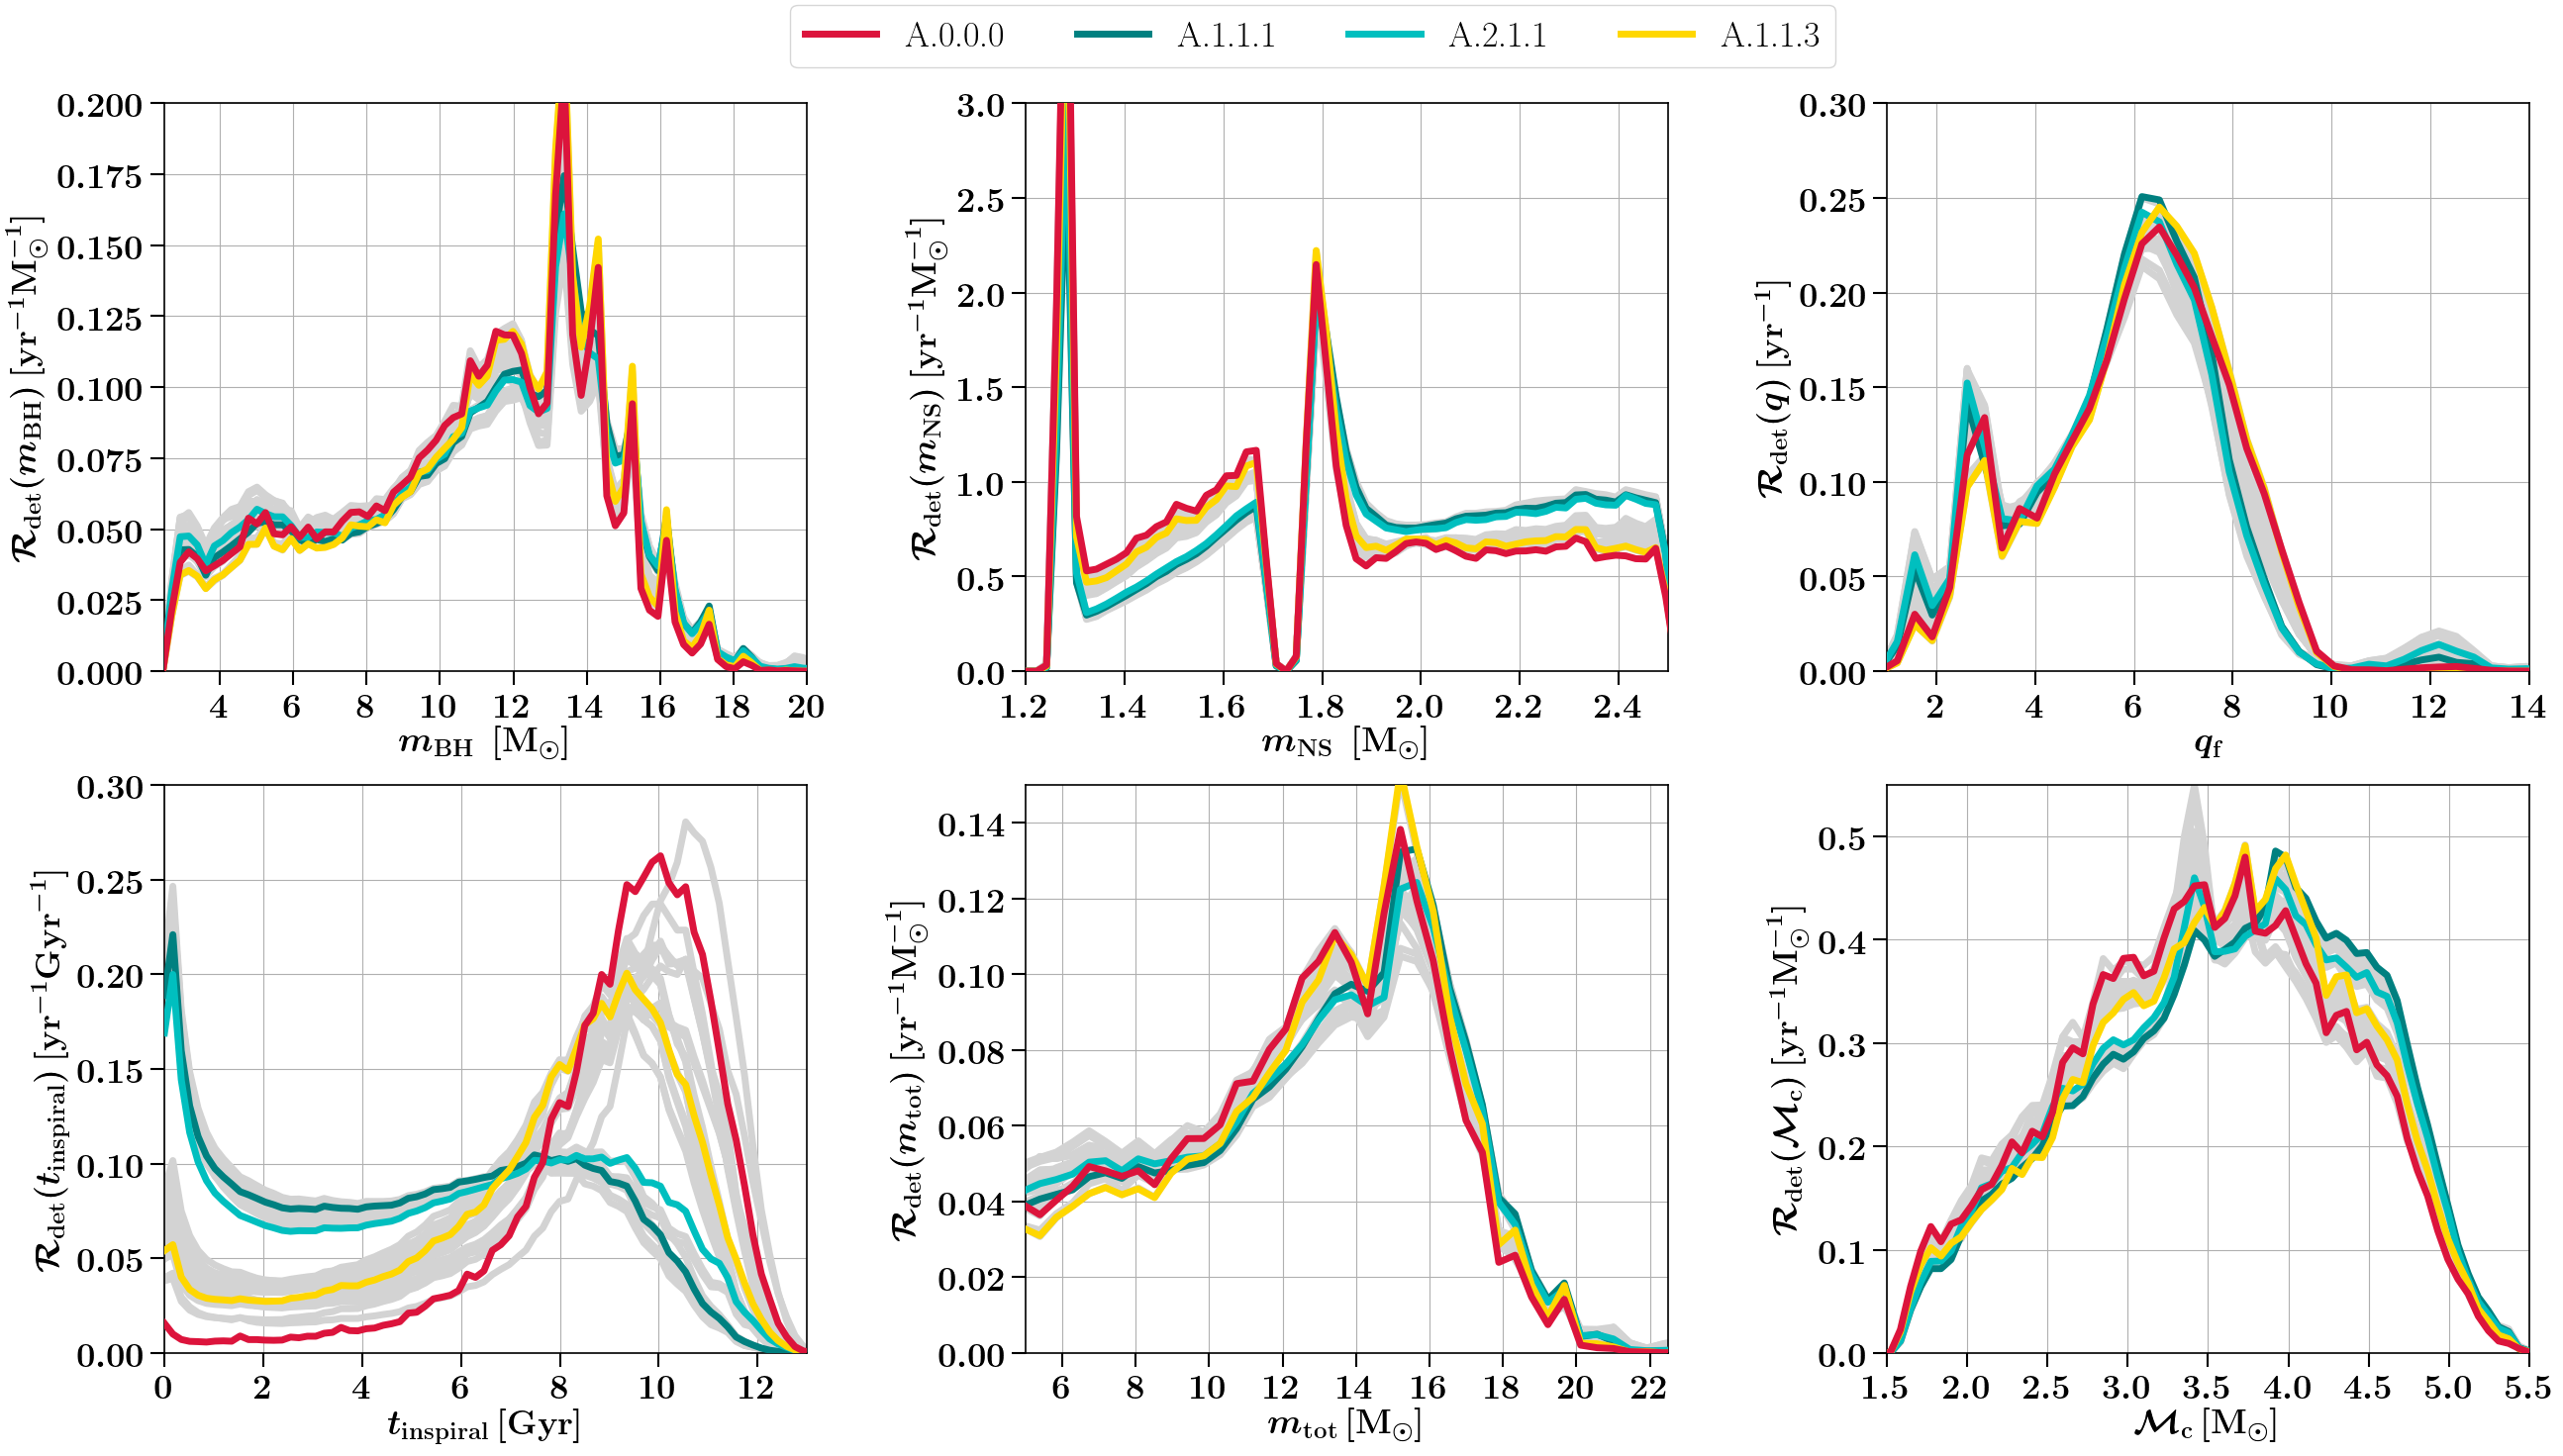
\includegraphics[width=1.0\textwidth]{../PlottingScripts/4_MSSFR_observed/ObservedDistributionsFiducial_MSSFR_gaussianKDE_highlight.png} %
    \caption{Normalized predicted distributions of the \bhnsSingle merger for advanced LIGO/Virgo for 28 different assumptions for our \ac{MSSFR} model (see Table~\ref{tab-MSSFR-variations-labels}).  }%
\end{figure*}
%




\section{Radii of stars at different metallicities}
\label{sec:app-radii-as-function-of-Z}
%
\begin{figure}
		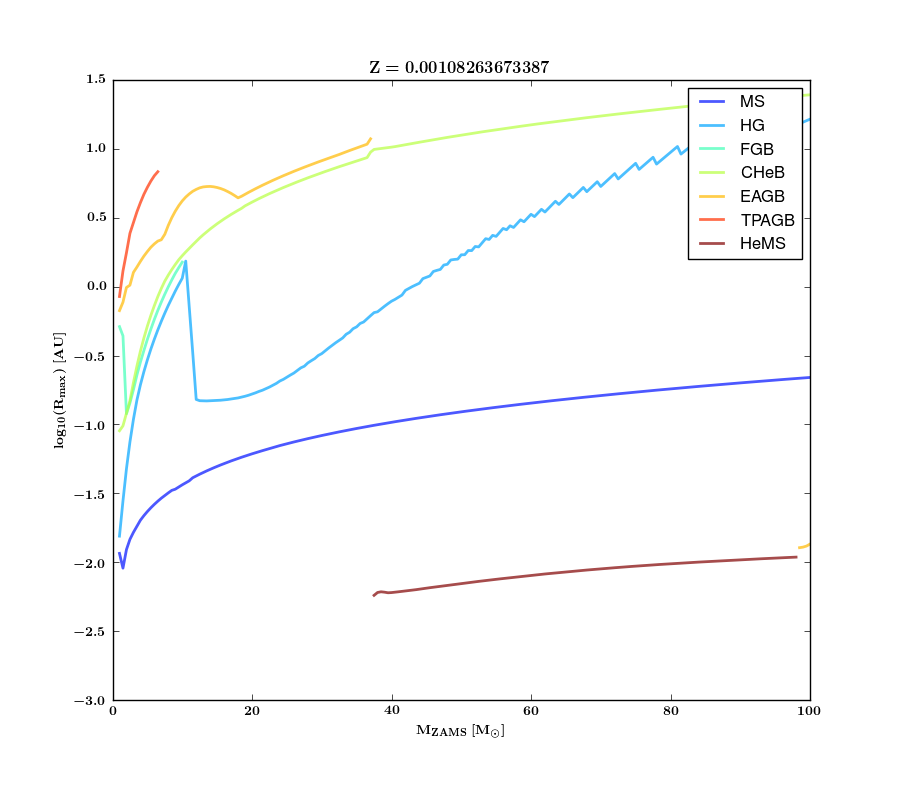
\includegraphics[width=.4\textwidth]{../OtherImages/12}
		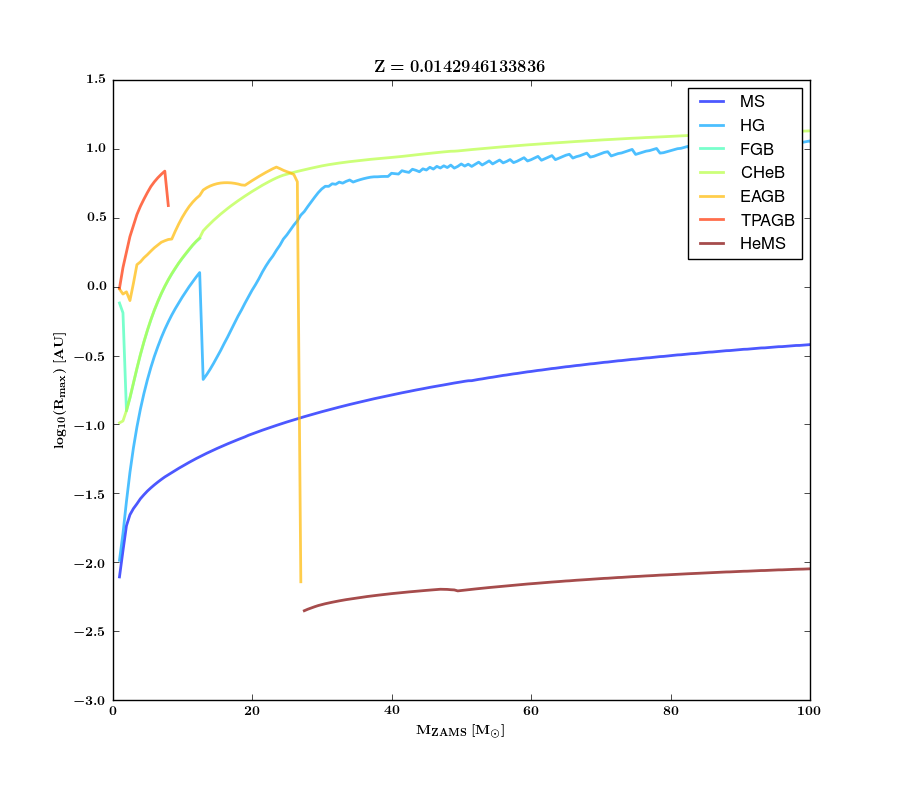
\includegraphics[width=.4\textwidth]{../OtherImages/25}
    \caption{ } 
    \label{fig:Radii-vs-metallicity}
\end{figure}


\section{metallicity of stars}

\begin{figure*}
\includegraphics[width=1\textwidth]{../PlottingScripts/7_Discussion/Metallicities_channels_BHNS.png}
   \caption{Metallicities of \bhnsSingle mergers observed with advanced LIGO   }
  \label{fig:BHNS_DCO_metallicities_observed_LIGO}
\end{figure*}
%


\section{Fiducial predictions for BHBH and NSNS mergers}
\label{sec:app-fiducial-GW-predictions-for-BBH-BNS}





\begin{figure*}
   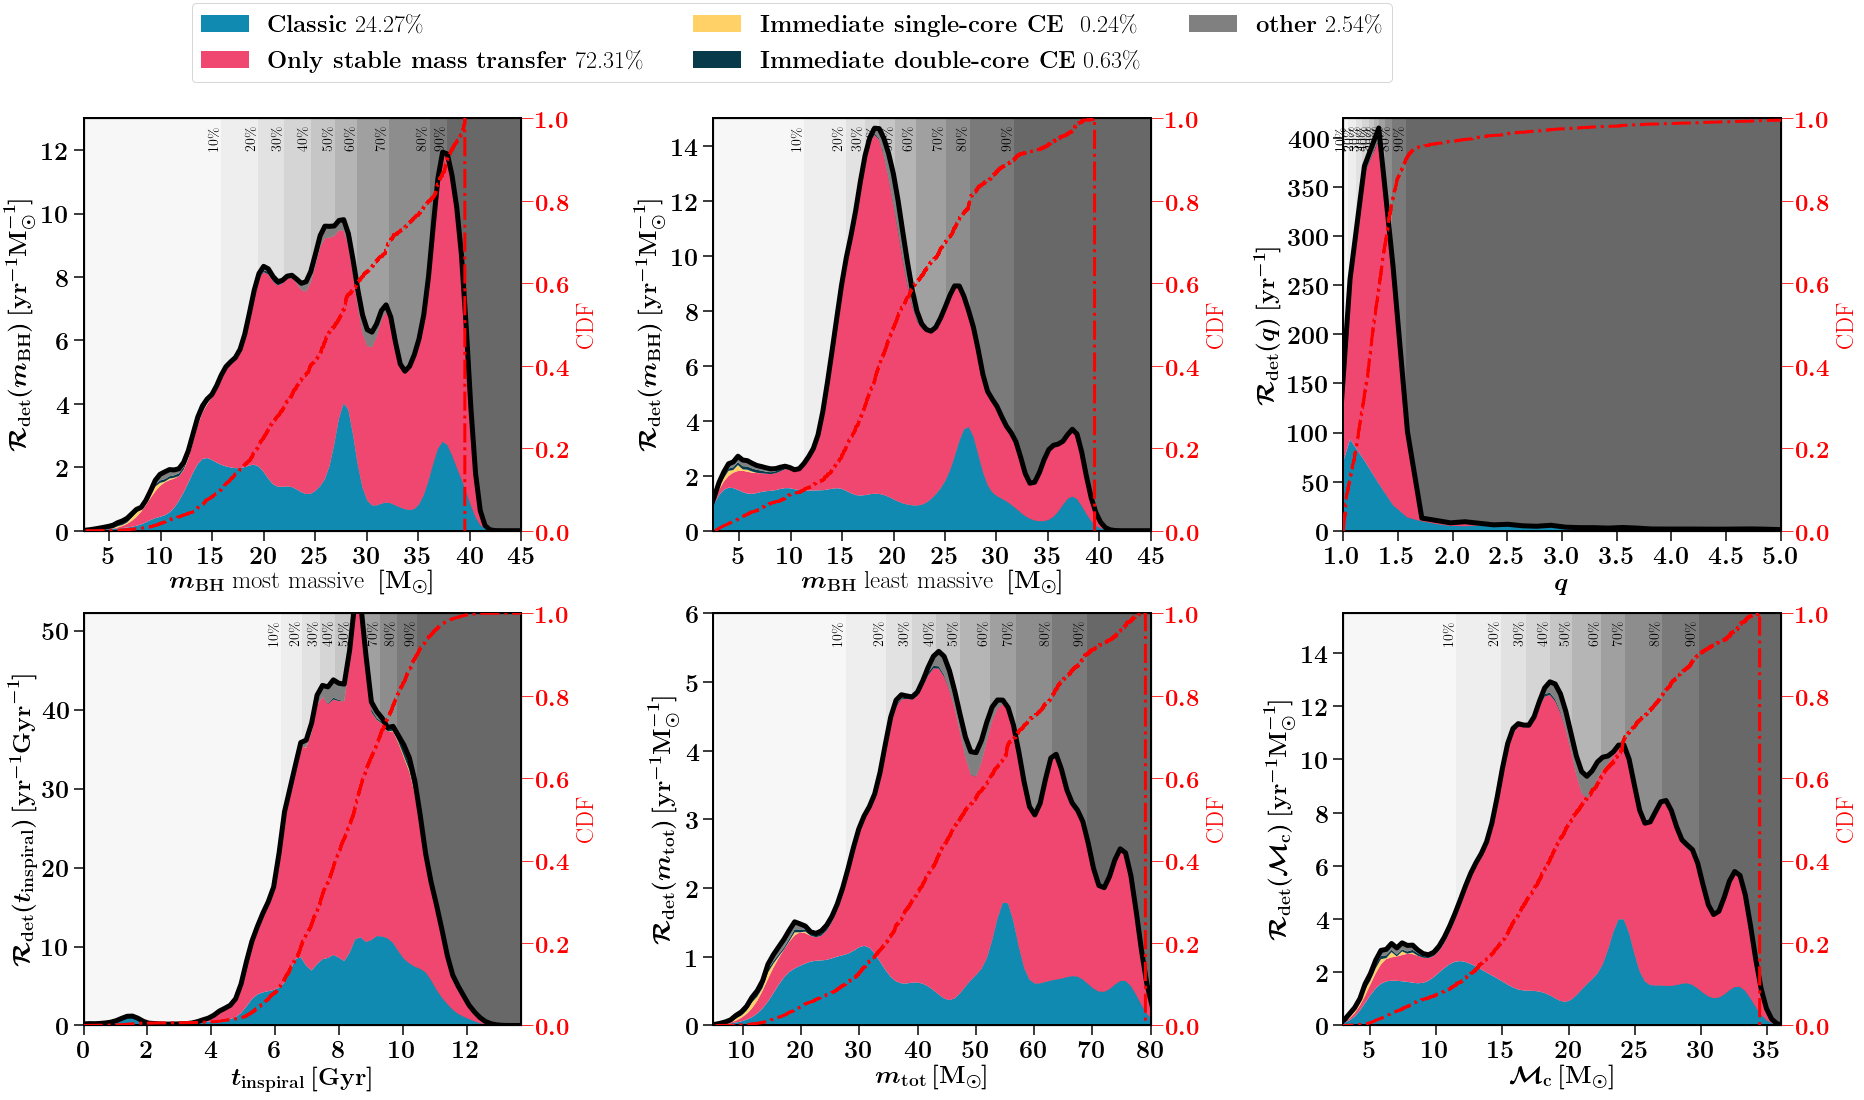
\includegraphics[width=1\textwidth]{../PlottingScripts/7_Discussion/DistributionsFiducialchannels_observed_BHBH.pdf}
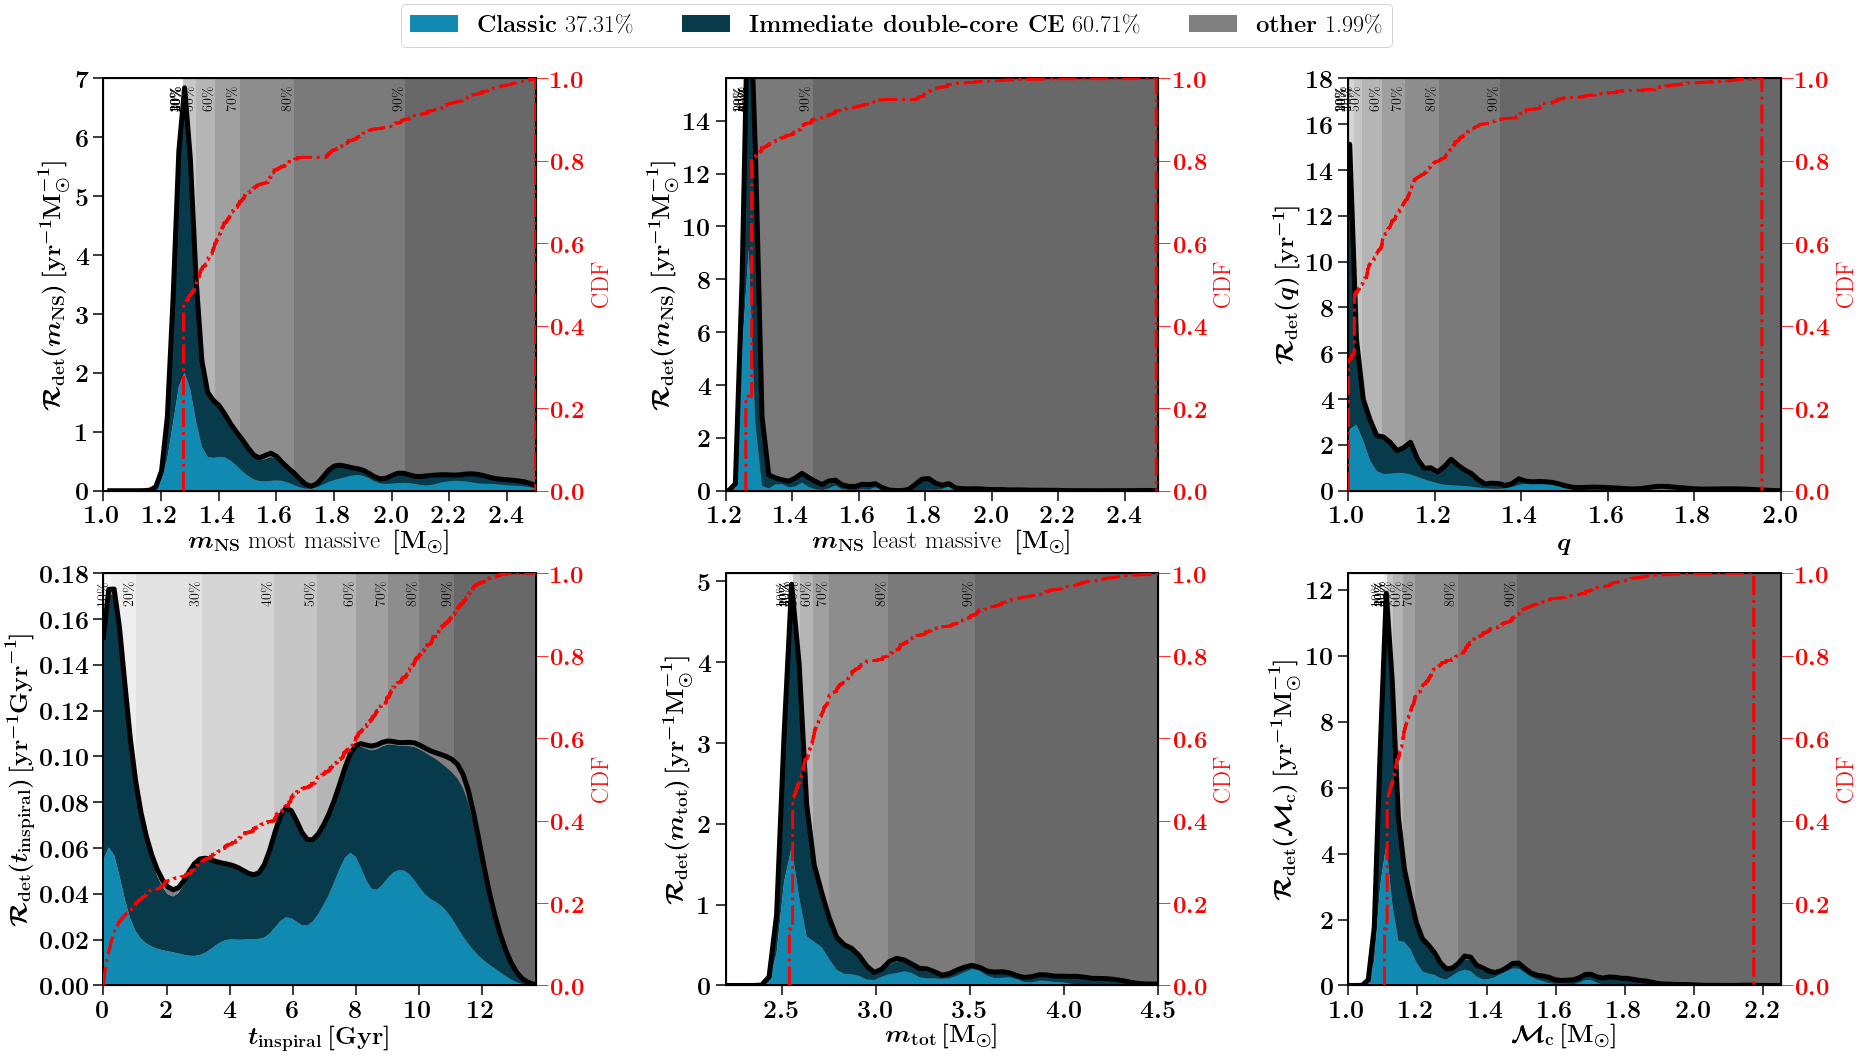
\includegraphics[width=1\textwidth]{../PlottingScripts/7_Discussion/DistributionsFiducialchannels_observed_NSNS.pdf}
      \caption{ Same as Figure~\ref{fig:BHNS_DCO_observed} but now for NSNS mergers in a Hubble time. }
  \label{fig:BHNS_DCO_observed_BNS}
\end{figure*}
%

\section{CDFs NSNS and BHBH}
\label{sec:app-BHBHandNSNS_CDF}


Number of BHBH mergers with low mass BHs is very dependent on model and MSSFR! So this will be a good prediction . 
Only optimistic model makes BHBHs with mass smaller than 5. 

Not so sensitive to even remnant mass function. 

mass ratio is very robust. 




%
\begin{figure*}
\label{fig:CDFs_BHNS_observed}
    \centering
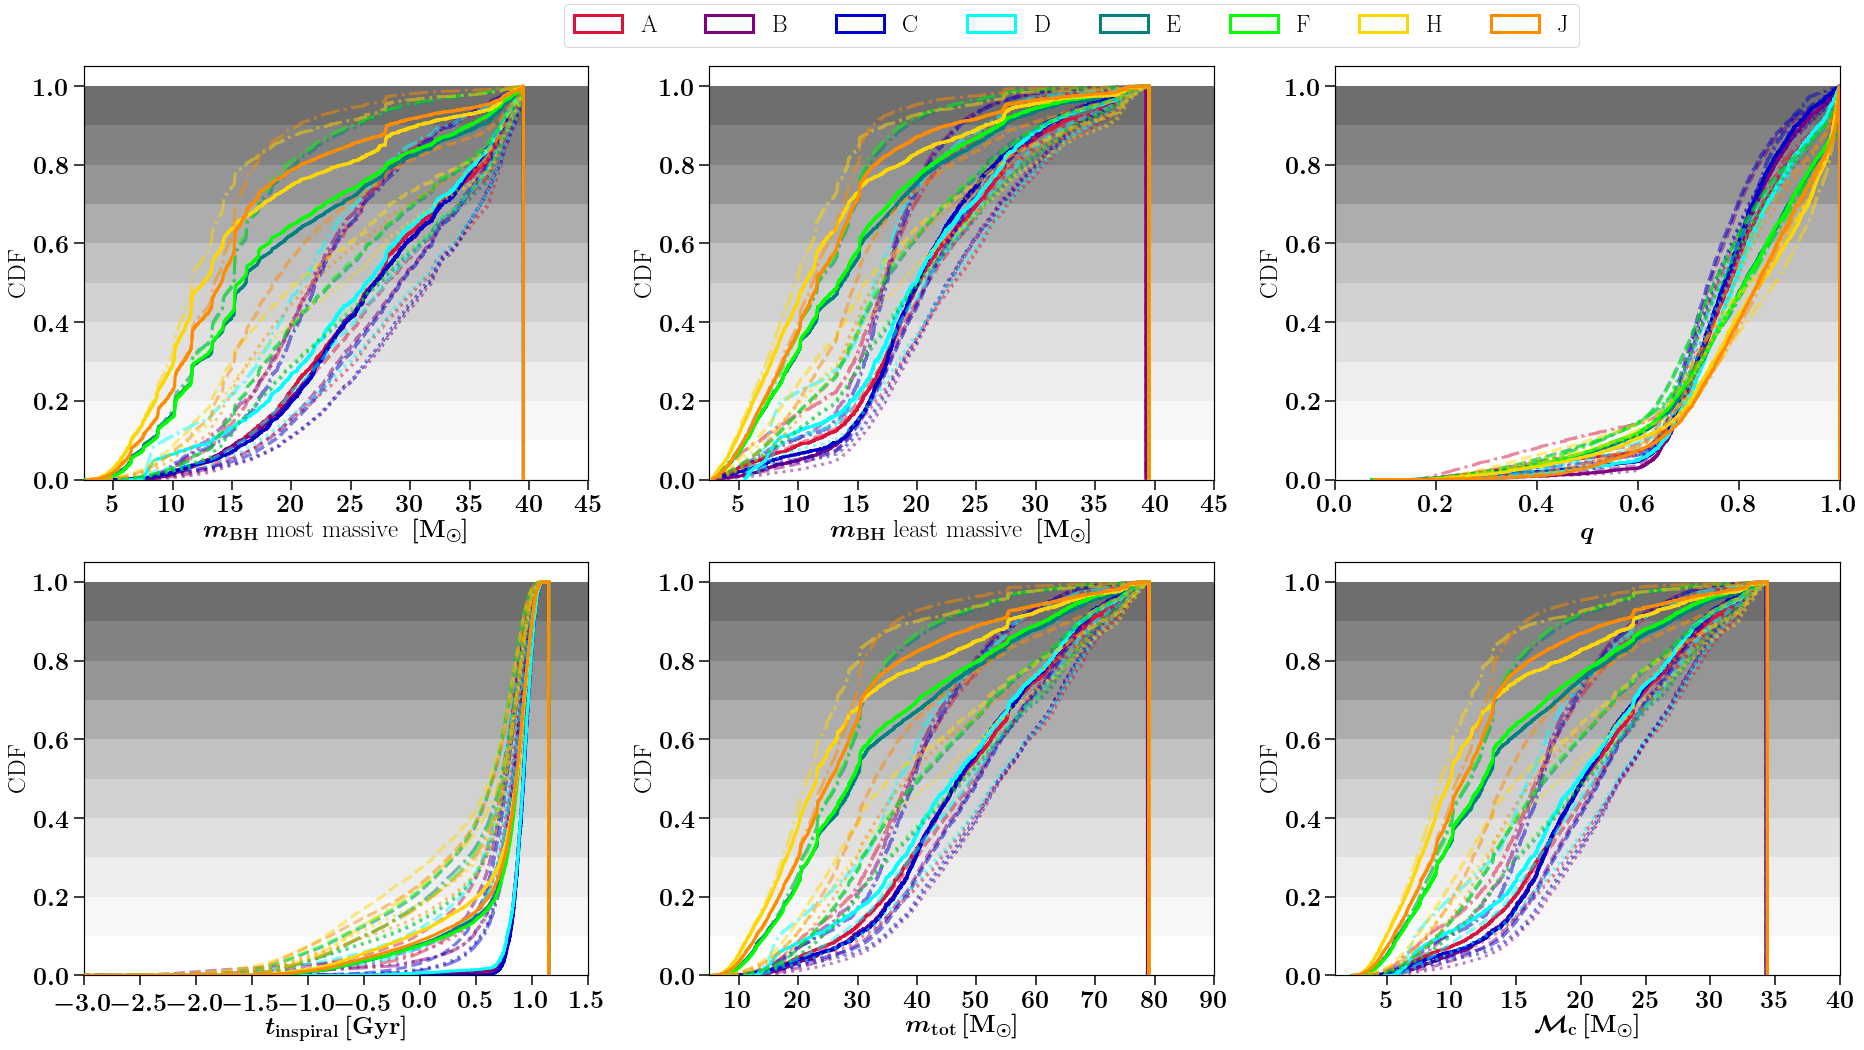
\includegraphics[width=1.0\textwidth]{../PlottingScripts/4_MSSFR_observed/DistributionsModels_observed_BHBH_CDF.pdf} %
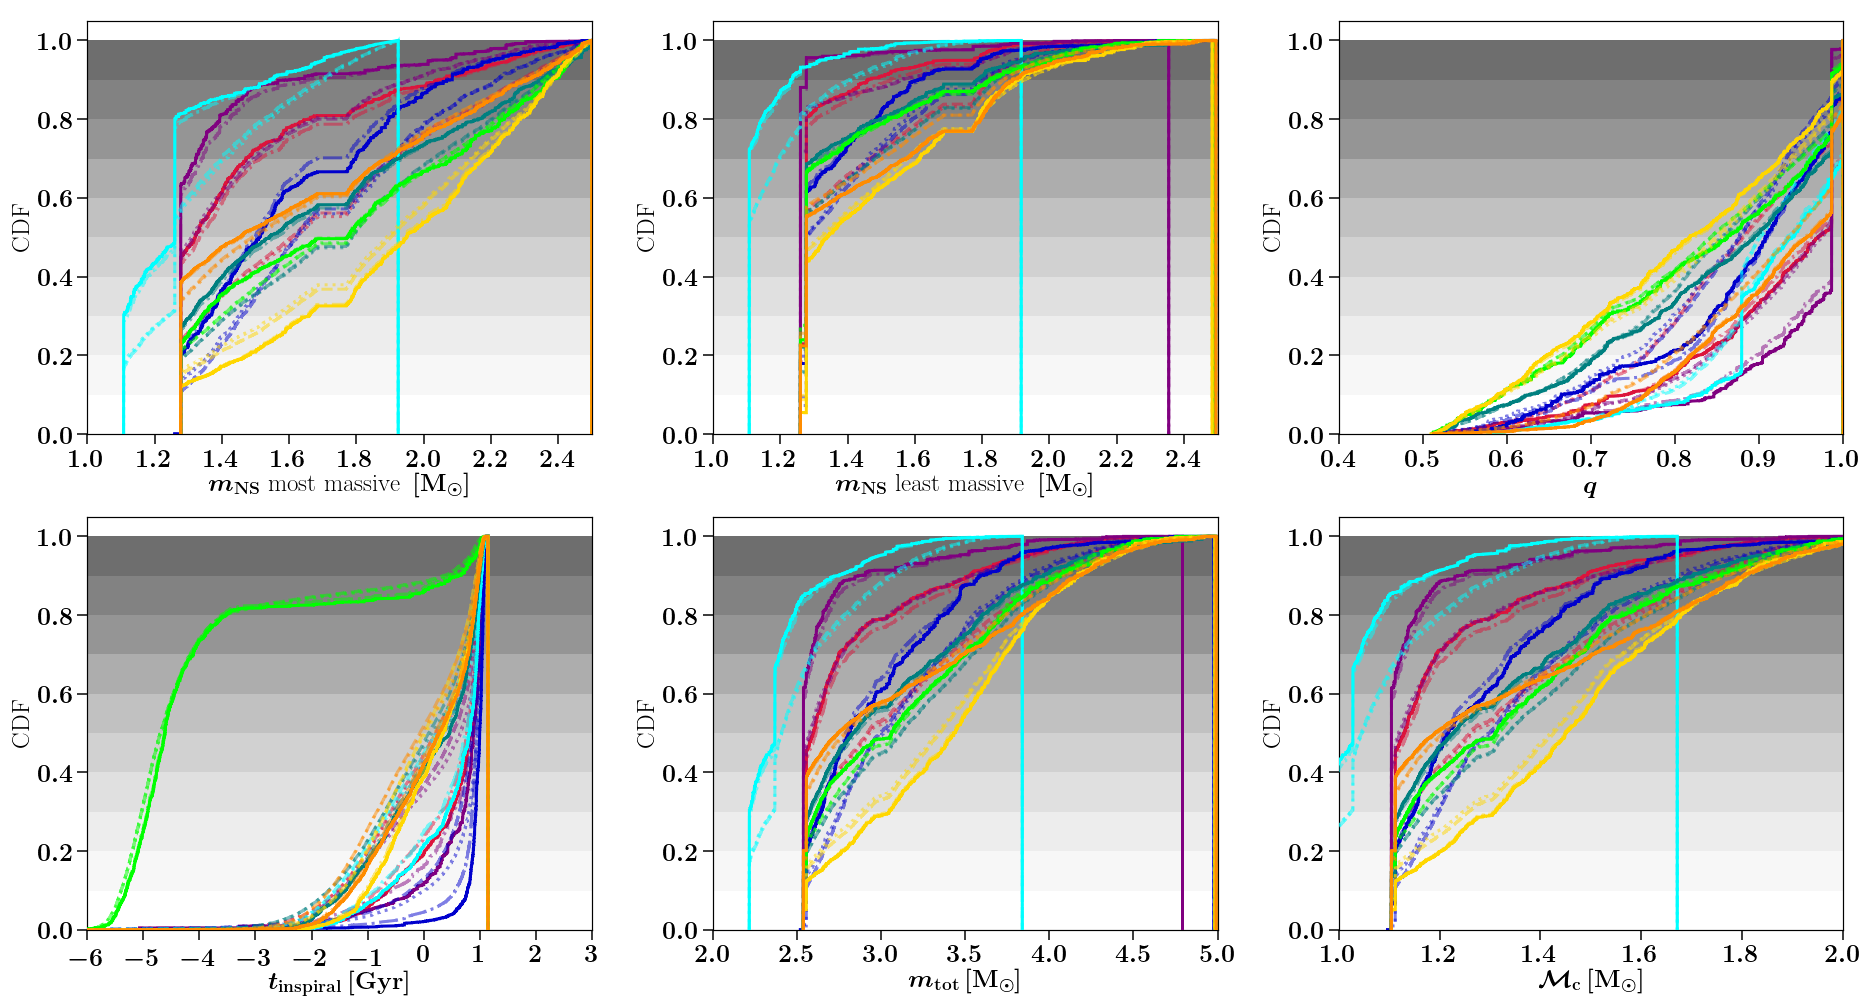
\includegraphics[width=1.0\textwidth]{../PlottingScripts/4_MSSFR_observed/DistributionsModels_observed_NSNS_CDF.pdf}
    \caption{}%
\end{figure*}
%


%
%%% FIGURE : fiducial LIGO PREDICTIONS 
%\begin{figure*}
%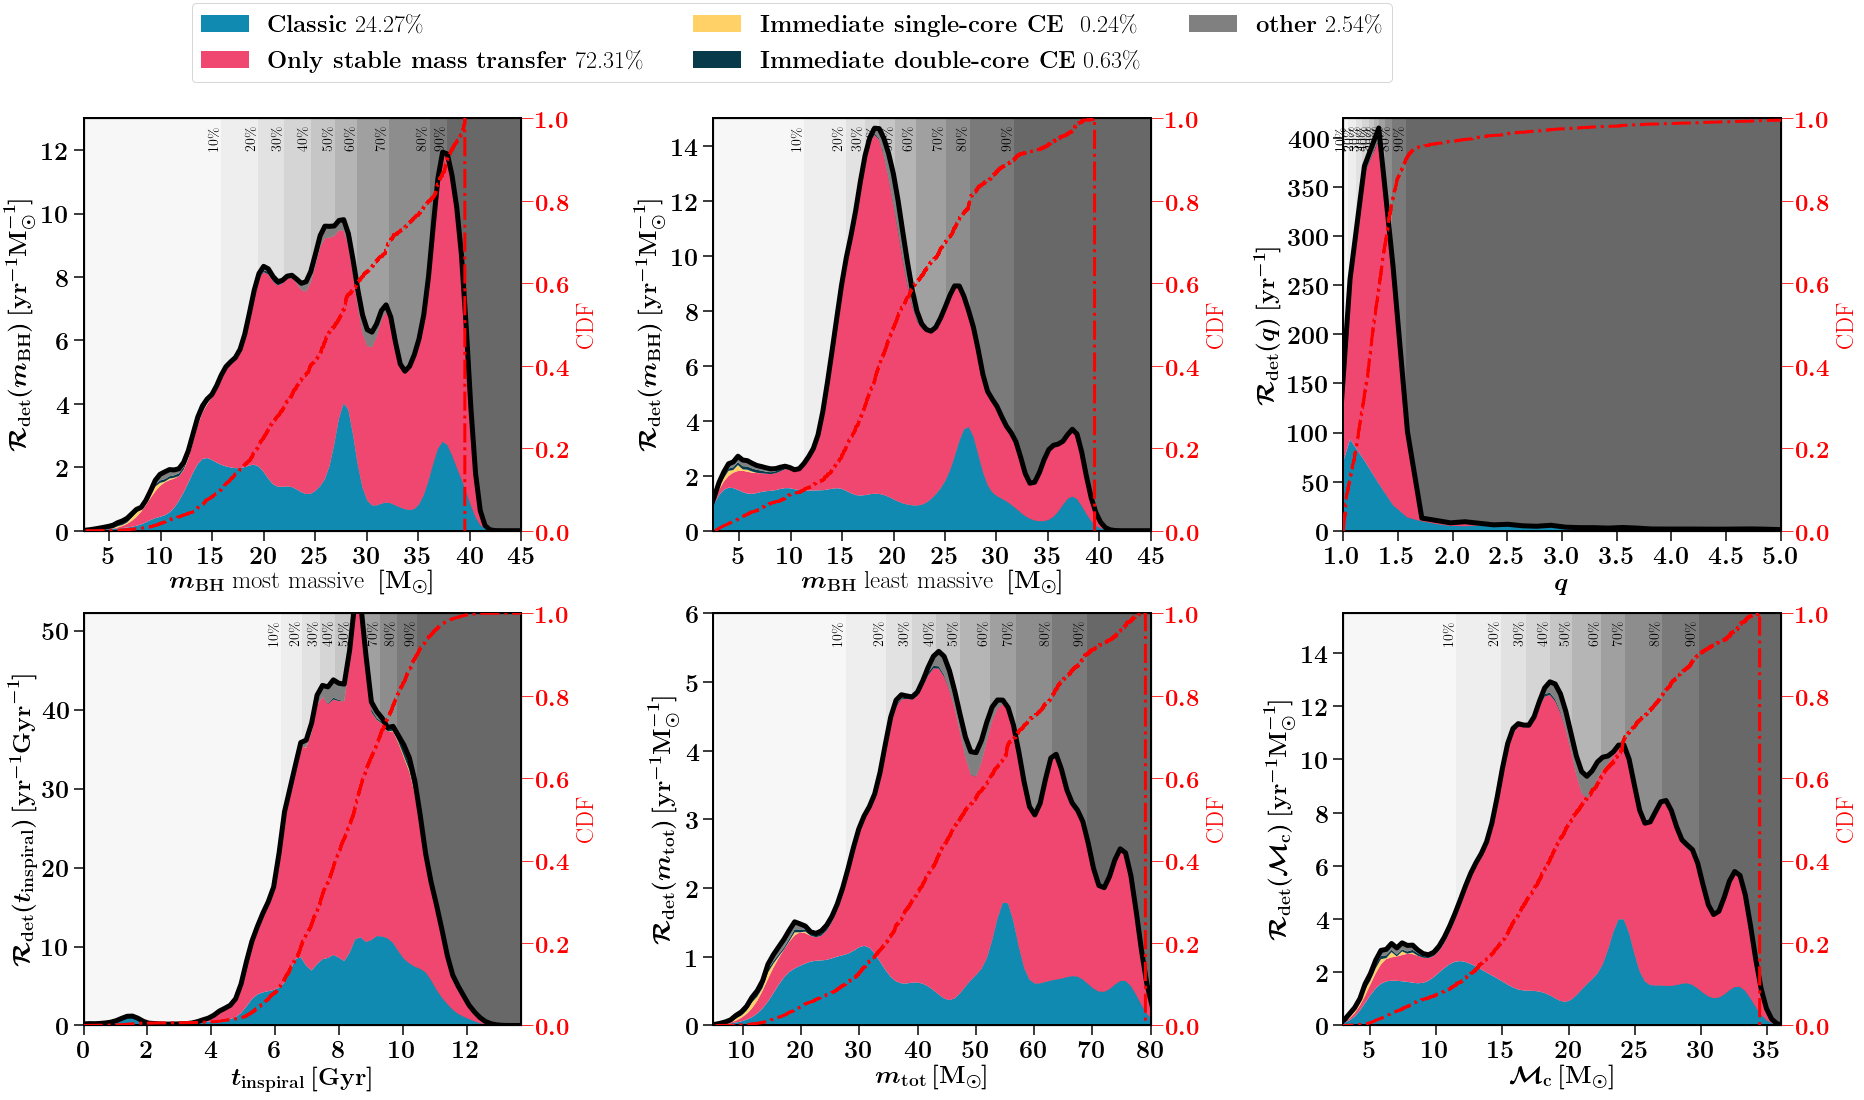
\includegraphics[width=1\textwidth]{../PlottingScripts/7_Discussion/DistributionsFiducialchannels_observed_BHBH.pdf}
%   \caption{ Same as Figure~\ref{fig:BHNS_DCO_observed} but now for BHBH mergers in a Hubble time. }
%  \label{fig:BHNS_DCO_observed_BBH}
%\end{figure*}
%%


%\section{Plots showing ZAMS masses for BHNS and NSBH seperate}
%%
%\begin{figure*}
%\includegraphics[width=\textwidth]{..PlottingScripts/3_DCO-Population/BHNS_ZAMSmasses_channels_combined_BHNS.png}
%   \caption{Progenitor masses of the binary systems forming a BH--NS binary ( \textbf{primary forms BH} )that mergers in a Hubble time for simulations at metallicity $Z=0.001$ [left],  and $Z=0.0142$ [right]. Colours represent different formation channels leading to the double compact object (see Sect.~\ref{subsec:results-Fiducial}). Each point or pixel represent one simulated binary system.  White areas are places in the parameter space where no BH--NS or NS--BH DCO form. }
%    \label{fig:BHNS_ZAMSmasses}
%\end{figure*}
%%
%
%%
%\begin{figure*}
%\includegraphics[width=\textwidth]{..PlottingScripts/3_DCO-Population/BHNS_ZAMSmasses_channels_combined_NSBH.png}
%   \caption{Progenitor masses of the binary systems forming a NS--BH (\textbf{primary forms NS}) binary that mergers in a Hubble time for simulations at metallicity $Z=0.001$ [left],  and $Z=0.0142$ [right]. Colours represent different formation channels leading to the double compact object (see Sect.~\ref{subsec:results-Fiducial}). Each point or pixel represent one simulated binary system.  White areas are places in the parameter space where no BH--NS or NS--BH DCO form. }
%    \label{fig:BHNS_ZAMSmasses}
%\end{figure*}
%%








\end{document}

% End of file `sample63.tex'.
